\documentclass[11pt,a4paper,english,greek,twoside]{ceid-thesis}
\let\cleardoublepage\clearpage

\usepackage{graphicx}
\graphicspath{{../../outputs/figures/}}
\usepackage{microtype}
\usepackage{indentfirst}
\usepackage{amsmath}
\usepackage{amsthm}
\usepackage{amssymb}
\usepackage{booktabs}
\usepackage{longtable}
\usepackage{tikz}
\usetikzlibrary{arrows.meta, positioning, shapes.geometric, calc}
\usepackage{algorithm}
\usepackage{algpseudocode}
\usepackage{hyperref}
\usepackage{bookmark}
\usepackage{csquotes}
\usepackage[backend=biber, style=apa]{biblatex}
\DeclareLanguageMapping{english}{american-apa}
\addbibresource{back_matter/references.bib}

\ifdefined\draftversion
  \usepackage{draftwatermark}
  \SetWatermarkText{\draftversion}
  \SetWatermarkScale{0.5}
  \SetWatermarkLightness{0.92}
\fi

\floatname{algorithm}{Αλγόριθμος}

\renewcommand{\baselinestretch}{1.2}
\setlength{\parskip}{4pt plus 2pt minus 1pt}

% Give the line breaker more room to avoid overfull boxes in paragraphs dense
% with long inline code identifiers, before falling back to an overfull line.
\tolerance=2000
\emergencystretch=2em

% Convenience commands
\newcommand{\en}[1]{\foreignlanguage{english}{#1}}
\newcommand{\src}[1]{\texttt{\en{#1}}}

% Allow line breaks after underscores in inline code/identifiers (\slash already
% does this for "/" in base LaTeX) so long src/ paths and function names in
% \texttt{\en{...}} don't overflow the margin.
\let\LPunderscore\_
\renewcommand{\_}{\LPunderscore\allowbreak}

% Auto-generated experiment macros (regenerate with: make generate-macros)
% AUTO-GENERATED by scripts/paper/generate_macros.py — do not edit by hand.
% Re-run: make thesis-macros

%% Dataset sizes
\newcommand{\TrainPairs}{948.232}
\newcommand{\TrainPairsNoSelf}{938.011}
\newcommand{\TrainSplitSize}{750.408}
\newcommand{\ValSplitSize}{187.603}
\newcommand{\TestPairs}{238.364}
\newcommand{\SvmSampleSize}{20.000}
\newcommand{\GraphNodes}{668.452}
\newcommand{\GraphMeanDegree}{1{,}30}
\newcommand{\GraphNodesTotal}{837.855}
\newcommand{\TrainPosCount}{435.843}
\newcommand{\TrainNegCount}{512.389}
\newcommand{\TrainPosPct}{46{,}0}
\newcommand{\TrainNegPct}{54{,}0}

%% Leakage audit
\newcommand{\LeakageExact}{2}
\newcommand{\LeakageExactPct}{0{,}0008}
\newcommand{\LeakageReversed}{301}
\newcommand{\LeakageReversedPct}{0{,}1263}
\newcommand{\SelfLoopsTrain}{10.221}
\newcommand{\SelfLoopsTrainPos}{10.220}
\newcommand{\SelfLoopsTrainNeg}{1}
\newcommand{\SelfLoopsTest}{2.553}
\newcommand{\IntraTrainDuplicates}{642}
\newcommand{\IntraTrainDuplicatesRows}{1.284}

%% Separability thresholds
\newcommand{\CnThreshold}{0{,}000}
\newcommand{\TfidfThreshold}{0{,}098}
\newcommand{\StructCnMeanPos}{0{,}00008}
\newcommand{\StructCnMeanNeg}{0{,}00000}
\newcommand{\StructTfidfMeanPos}{0{,}229}
\newcommand{\StructTfidfMeanNeg}{0{,}022}
\newcommand{\GraphCoverageTrainPct}{46{,}34}
\newcommand{\GraphCoverageTestPct}{1{,}72}

%% Difficulty — train
\newcommand{\TrainDiffSelfLoopN}{10.221}
\newcommand{\TrainDiffSelfLoopPct}{1{,}08}
\newcommand{\TrainDiffHighCnN}{36}
\newcommand{\TrainDiffHighCnPct}{0{,}00}
\newcommand{\TrainDiffHighTextsimN}{330.111}
\newcommand{\TrainDiffHighTextsimPct}{34{,}81}
\newcommand{\TrainDiffHardN}{607.864}
\newcommand{\TrainDiffHardPct}{64{,}10}
\newcommand{\TrainDiffTrivialPct}{35{,}90}

%% Difficulty — test
\newcommand{\TestDiffSelfLoopN}{2.553}
\newcommand{\TestDiffSelfLoopPct}{1{,}07}
\newcommand{\TestDiffHighCnN}{5}
\newcommand{\TestDiffHighTextsimN}{82.646}
\newcommand{\TestDiffHighTextsimPct}{34{,}67}
\newcommand{\TestDiffHardN}{153.160}
\newcommand{\TestDiffHardPct}{64{,}25}

%% Reproducibility & hyperparameters
\newcommand{\Seed}{42}
\newcommand{\ValSizeFrac}{0{,}2}
\newcommand{\ValSizePct}{20{,}0}
\newcommand{\StructuralC}{1{,}0}
\newcommand{\StructuralMaxIter}{1.000}
\newcommand{\TfidfClfC}{1{,}0}
\newcommand{\TfidfClfMaxIter}{1.000}
\newcommand{\PosNEstimators}{200}
\newcommand{\PosClassWeight}{balanced}
\newcommand{\EmbeddingC}{1{,}0}
\newcommand{\EmbeddingMaxIter}{1.000}
\newcommand{\SvmC}{1{,}0}
\newcommand{\SvmGamma}{scale}
\newcommand{\TfidfMaxFeatures}{50.000}
\newcommand{\TfidfSublinearTf}{True}
\newcommand{\TfidfMinDf}{2}
\newcommand{\EmbeddingModelName}{all-MiniLM-L6-v2}
\newcommand{\NTwoVDimensions}{64}
\newcommand{\NTwoVWalkLength}{30}
\newcommand{\NTwoVNumWalks}{10}
\newcommand{\NTwoVWindow}{10}
\newcommand{\NTwoVP}{1}
\newcommand{\NTwoVQ}{1}

%% Cascade thresholds
\newcommand{\TauOneDefault}{0{,}8}
\newcommand{\TauTwoDefault}{0{,}7}
\newcommand{\NTwoVDim}{68}

%% Cascade val results
\newcommand{\CascadeValFone}{0{,}9986}
\newcommand{\CascadeValAuc}{0{,}9998}
\newcommand{\TierOneCount}{36.352}
\newcommand{\TierOnePct}{19{,}38}
\newcommand{\TierOneAcc}{0{,}9985}
\newcommand{\TierOneFone}{0{,}4996}
\newcommand{\TierTwoCount}{151.160}
\newcommand{\TierTwoPct}{80{,}57}
\newcommand{\TierTwoAcc}{0{,}9991}
\newcommand{\TierTwoFone}{0{,}9989}
\newcommand{\TierThreeCount}{91}
\newcommand{\TierThreePct}{0{,}05}
\newcommand{\TierThreeAcc}{0{,}2857}
\newcommand{\TierThreeFone}{0{,}2802}
\newcommand{\TierOnePosPct}{99{,}85}
\newcommand{\TierThreeTruePosPct}{78{,}0}
\newcommand{\TierThreePredPosPct}{30{,}8}

%% Tier x difficulty
\newcommand{\TierOneHardN}{11.455}
\newcommand{\TierOneHardAcc}{0{,}9954}
\newcommand{\TierOneHighTextsimN}{24.890}
\newcommand{\TierOneHighTextsimAcc}{1{,}0000}
\newcommand{\TierOneHighCnN}{7}
\newcommand{\TierOneHighCnAcc}{1{,}0000}
\newcommand{\TierTwoHardN}{110.325}
\newcommand{\TierTwoHardAcc}{0{,}9989}
\newcommand{\TierTwoHighTextsimN}{40.835}
\newcommand{\TierTwoHighTextsimAcc}{0{,}9996}
\newcommand{\TierThreeHardN}{78}
\newcommand{\TierThreeHardAcc}{0{,}1667}
\newcommand{\TierThreeHighTextsimN}{13}
\newcommand{\TierThreeHighTextsimAcc}{1{,}0000}

%% Test-set tier dist
\newcommand{\TestTierOneCount}{943}
\newcommand{\TestTierOnePct}{0{,}4}
\newcommand{\TestTierZeroPct}{1{,}1}
\newcommand{\TestTierTwoPct}{98{,}5}

%% Cold-start
\newcommand{\ColdStartCount}{151.251}
\newcommand{\ColdStartPct}{80{,}6229}
\newcommand{\ColdStartNonCount}{36.352}

%% Hard residual
\newcommand{\HardResCount}{78}
\newcommand{\HardResAcc}{0{,}1667}
\newcommand{\HardResMissingN}{60}
\newcommand{\HardResMissingPct}{76{,}9}
\newcommand{\HardResCompleteN}{18}
\newcommand{\HardResCompleteAcc}{0{,}1667}
\newcommand{\HardResIncompleteAcc}{0{,}1667}
\newcommand{\HardResNodeId}{415071}
\newcommand{\HardResNodePairs}{18}
\newcommand{\HardResNodePredPosPct}{55{,}6}

%% Efficiency
\newcommand{\ThroughputSec}{1{,}83}
\newcommand{\ThroughputRate}{102.299}
\newcommand{\ThroughputLatency}{0{,}010}
\newcommand{\TierThreeCallRateMax}{0{,}674}

%% Error analysis
\newcommand{\CascadeTotalErrors}{261}
\newcommand{\CascadeErrorsHardN}{244}
\newcommand{\CascadeErrorsHardPct}{93{,}49}
\newcommand{\CascadeErrorsTrivialN}{17}
\newcommand{\CascadeErrorsTrivialPct}{6{,}51}
\newcommand{\CascadeHardAcc}{0{,}9980}
\newcommand{\CascadeHardFone}{0{,}9964}
\newcommand{\SvmTotalErrors}{16.696}
\newcommand{\CascadeVsSvmRatio}{64}
\newcommand{\SvmErrorsHardN}{15.631}
\newcommand{\SvmErrorsHardPct}{93{,}62}
\newcommand{\SvmErrorsTrivialN}{1.065}
\newcommand{\SvmErrorsTrivialPct}{6{,}38}
\newcommand{\SvmHighTextsimAcc}{0{,}9838}
\newcommand{\SvmHighTextsimFone}{0{,}4959}
\newcommand{\SvmHardAcc}{0{,}8717}
\newcommand{\SvmHardFone}{0{,}7033}

%% Node2Vec ablation
\newcommand{\NTwoVWithCallPct}{99{,}30}
\newcommand{\NTwoVWithCallN}{186.298}
\newcommand{\NTwoVWithOverallFone}{0{,}9958}
\newcommand{\NTwoVWithConfFone}{0{,}9970}
\newcommand{\NTwoVNoOverallFone}{0{,}7693}
\newcommand{\NTwoVNoConfFone}{0{,}4996}
\newcommand{\NTwoVNoAccOverall}{0{,}7900}
\newcommand{\NTwoVWithAccOverall}{0{,}9958}
\newcommand{\NTwoVIdOneCoverage}{9{,}4}
\newcommand{\NTwoVIdTwoCoverage}{30{,}3}
\newcommand{\NTwoVZeroVecPct}{98{,}3}
\newcommand{\NTwoVZeroVecN}{234.276}
\newcommand{\NTwoVTestTierOnePct}{98{,}6}

%% Threshold ablation
\newcommand{\AblGridPoints}{25}
\newcommand{\AblTierOneLowFone}{0{,}9973}
\newcommand{\AblTierOneHighFone}{0{,}9976}
\newcommand{\AblTierOneLowPct}{24{,}69}
\newcommand{\AblTierOneBreakPct}{19{,}38}
\newcommand{\AblTierOneBreakPctHigh}{17{,}47}
\newcommand{\AblBestFone}{0{,}9987}
\newcommand{\AblDefaultFone}{0{,}9986}
\newcommand{\AblHighTauOneLowFone}{0{,}9983}
\newcommand{\AblTauTwoMaxTierThreePct}{0{,}66}
\newcommand{\AblTThreeRateZeroFive}{0{,}000}
\newcommand{\AblTThreeRateZeroSix}{0{,}021}
\newcommand{\AblTThreeRateZeroSeven}{0{,}049}
\newcommand{\AblTThreeRateZeroEight}{0{,}156}
\newcommand{\AblTThreeRateZeroNine}{0{,}659}

%% SVM baseline
\newcommand{\SvmFone}{0{,}9091}
\newcommand{\SvmAuc}{0{,}9431}
\newcommand{\SvmCsFone}{0{,}9091}
\newcommand{\SvmLatency}{0{,}46191}

%% Kaggle scores
\newcommand{\KaggleBaselinePublic}{0{,}99831}
\newcommand{\KaggleBaselinePrivate}{0{,}99828}
\newcommand{\NTwoVKagglePublic}{0{,}38879}
\newcommand{\NTwoVKagglePrivate}{0{,}38910}

%% Additional computed macros
\newcommand{\AblForceExtraPoints}{20}
\newcommand{\AblForceFoneDrop}{0{,}0214}
\newcommand{\AblForceGridPoints}{45}
\newcommand{\AblForceModerateFone}{0{,}9888}
\newcommand{\AblForceModerateTierThreeFone}{0{,}8938}
\newcommand{\AblForceModerateTierThreePct}{11{,}16}
\newcommand{\AblForcePlateauFone}{0{,}9772}
\newcommand{\AblForcePlateauTierThreeFone}{0{,}9195}
\newcommand{\AblForcePlateauTierThreePct}{27{,}67}
\newcommand{\AblForcePlateauTierTwoPct}{52{,}95}
\newcommand{\AblForceTierThreeFoneGain}{0{,}6394}
\newcommand{\EmbeddingAuc}{0{,}9576}
\newcommand{\EmbeddingCsFone}{0{,}9058}
\newcommand{\EmbeddingFone}{0{,}9058}
\newcommand{\TierThreeHighCnAcc}{---}
\newcommand{\TierThreeHighCnN}{0}
\newcommand{\TierTwoHighCnAcc}{---}
\newcommand{\TierTwoHighCnN}{0}
\newcommand{\TierTwoSatCeilingPct}{65{,}68}
\newcommand{\TierTwoSatEligibleN}{151.251}
\newcommand{\TierTwoSatEligiblePct}{80{,}62}
\newcommand{\TierTwoSatNEstimators}{200}
\newcommand{\TierTwoSatNonSaturatedPct}{34{,}32}


% Theorem environments (English)
\newtheorem{definition}{Definition}
\newtheorem{theorem}{Theorem}
\newtheorem{proposition}{Proposition}
\newtheorem{lemma}{Lemma}
\newtheorem{corollary}{Corollary}
\renewcommand{\thedefinition}{\arabic{chapter}.\arabic{definition}}
\renewcommand{\thetheorem}{\arabic{chapter}.\arabic{theorem}}

%%%%%%%%%%%%%%%%%%%%%%%%%%%%%%%%%%%%%%%%%%%%%%%%%%%%%
%% THESIS INFO — fill in before submission
%%
\title{Πρόβλεψη Συνδέσμων σε Γραφήματα με Χαρακτηριστικά Κειμένου}
\edef\toutis{του}
\edef\authorNameCapital{ΓΚΟΝΗΣ ΓΕΩΡΓΙΟΣ}
\author{Γεώργιος Γκόνης}
\supervisor{Χρήστος Μακρής}
\edef\supervisorTitle{Καθηγητής}
\supervisorSecond{}
\edef\supervisorSecondTitle{}
\edef\supervisorMaleFemale{Επιβλέπων}
\edef\thesisPlaceDate{Πάτρα, Ιούλιος 2026}
\edef\examinationDate{Ιούλιο 2026}
\edef\copyrightYear{2026}
\epitropiF{Σπύρος Σιούτας}
\edef\epitropiFTitle{Καθηγητής}
\epitropiS{Κωνσταντίνος Τσίχλας}
\edef\epitropiSTitle{Καθηγητής}
%%%%%%%%%%%%%%%%%%%%%%%%%%%%%%%%%%%%%%%%%%%%%%%%%%%%%

\begin{document}
    \selectlanguage{greek}
    \maketitle

    \frontmatter
    % Greek abstract
\begin{abstract}
    Η πρόβλεψη ακμών σε γραφήματα με κειμενικά χαρακτηριστικά κόμβων αποτελεί το πρόβλημα
    εξαγωγής συμπεράσματος για την ύπαρξη ακμής μεταξύ δύο κόμβων, λαμβάνοντας υπόψη
    τόσο την τοπολογία του γραφήματος όσο και το κειμενικό περιεχόμενο των κόμβων.
    Πρόσφατες εργασίες σε τέτοια γραφήματα έχουν αναφέρει σχεδόν τέλεια ακρίβεια με
    καθαρά σημασιολογικές προσεγγίσεις βασισμένες σε προ-εκπαιδευμένα γλωσσικά
    μοντέλα, όμως το τετραγωνικό κόστος συμπερασμού τους τα καθιστά μη πρακτικά σε
    κλίμακα.

    Η παρούσα διπλωματική εργασία προτείνει το \textbf{\en{CascadeLP}}, ένα
    τετραεπίπεδο πλαίσιο πρόβλεψης ακμών που αντιμετωπίζει το κόστος συμπερασμού ως
    πρωταρχικό σχεδιαστικό περιορισμό: δρομολογεί κάθε ζεύγος κόμβων μέσω προοδευτικά
    πιο δαπανηρών μοντέλων βάσει ορίων αξιοπιστίας, κλιμακώνοντας μόνο όταν το
    φθηνότερο επίπεδο δεν είναι αρκετά σίγουρο.
    Η αλυσίδα περιλαμβάνει: αυτοβρόχους,
    δομικούς ευρετικούς δείκτες (\en{Common Neighbours}, \en{Jaccard},
    \en{Adamic-Adar}, \en{Preferential Attachment}), συχνότητες μερών του λόγου με
    \en{Random Forest} για κόμβους χωρίς δομικούς γείτονες, και έναν κωδικοποιητή
    \en{Sentence-Transformer} για ζεύγη στα οποία τα προηγούμενα επίπεδα εμφανίζουν
    αβεβαιότητα.

    Αξιολογούμε το \en{CascadeLP} στο σύνολο αξιολόγησης \en{DSAA 2023} της
    \en{Wikipedia}, το οποίο επιλέγεται ως πεδίο αξιολόγησης επειδή συνιστά
    ρεαλιστικό στιγμιότυπο γραφήματος με κειμενικά χαρακτηριστικά σε κλίμακα
    εκατοντάδων χιλιάδων κόμβων, με καθιερωμένο πίνακα κατάταξης διαγωνισμού που
    παρέχει υπαρκτές λύσεις προς σύγκριση.
    Για να επικυρώσουμε ότι η επιτυγχανόμενη
    ακρίβεια είναι γνήσια και όχι τεχνούργημα διαρροής δεδομένων ή τετριμμένης
    διαχωρισιμότητας, διεξάγουμε έναν συστηματικό έλεγχο \en{data leakage} --- που
    βρίσκει αμελητέα επικάλυψη ζευγών --- και έναν ανεξάρτητο χαρακτηρισμό
    διαχωρισιμότητας του συνόλου δεδομένων, τον οποίο διασταυρώνουμε ανά ζεύγος με το
    επίπεδο που το επέλυσε.
    Το \en{CascadeLP} πετυχαίνει \en{Macro F1} = \CascadeValFone{}
    σε πλήρως ανεξάρτητο σύνολο επικύρωσης --- επιβεβαιωμένο ανεξάρτητα με
    \en{Macro F1} = \KaggleBaselinePublic{} στο δημόσιο \en{leaderboard} του
    διαγωνισμού --- καλώντας τον ακριβό κωδικοποιητή \en{Sentence-Transformer} σε
    μόλις \TierThreePct\% των ζευγών.
    Συμπεριλαμβάνουμε επίσης ένα μοντέλο αναφοράς
    \en{TF-IDF + SVM}.
    Η γενίκευση σε δεύτερο σύνολο δεδομένων αναβάλλεται ως
    μελλοντική εργασία.

    \begin{keywords}
        Πρόβλεψη ακμών, γραφήματα με κειμενικά χαρακτηριστικά, νευρωνικά δίκτυα γραφημάτων,
        γλωσσικά μοντέλα, βαθμιδωτή συμπερασματολογία, \en{cold-start},
        \en{Wikipedia}, \en{DSAA 2023}
    \end{keywords}
\end{abstract}

% English abstract
\begin{abstracteng}
    \en{
        Link prediction in text-attributed graphs (TAGs) is the problem of inferring whether an
        edge exists between two nodes given both the graph topology and the textual content of
        the nodes. Recent work on such graphs has reported near-perfect accuracy with pure
        semantic approaches based on pre-trained language models, but their quadratic inference
        cost makes them impractical at scale.

        This thesis proposes \textbf{CascadeLP}, a four-tier link prediction framework that
        treats inference cost as a first-class design constraint: it routes each node pair
        through progressively more expensive models based on confidence thresholds, escalating
        only when the cheaper tier is not confident enough. The cascade includes: self-loops,
        structural heuristics (Common Neighbours, Jaccard, Adamic-Adar, Preferential
        Attachment), POS-tag frequency features with a Random Forest for nodes with no
        structural neighbours, and a Sentence-Transformer encoder for pairs where the earlier
        tiers remain uncertain.

        We evaluate CascadeLP on the DSAA 2023 Wikipedia benchmark, selected as our evaluation
        scope because it is a realistic, large-scale text-attributed graph with an established
        competition leaderboard of existing solutions to benchmark against. To validate that the
        achieved accuracy is genuine rather than an artifact of data leakage or trivial dataset
        separability, we run a systematic leakage audit -- which finds negligible pair overlap --
        and an independent dataset separability characterization, cross-referenced per pair with
        the tier that resolved it. CascadeLP achieves Macro F1 = \CascadeValFone{} on a fully
        held-out validation set -- independently confirmed with Macro F1 = \KaggleBaselinePublic{}
        on the competition's public leaderboard -- while calling the expensive
        Sentence-Transformer encoder on only \TierThreePct\% of pairs. We also include a TF-IDF
        + SVM reference baseline. Generalization to a second dataset is deferred to
        future work. }

    \begin{keywordseng}
        \en{Link prediction, text-attributed graphs, graph neural networks, language models,
            cascaded inference, cold-start, Wikipedia, DSAA 2023}
    \end{keywordseng}
\end{abstracteng}
            % Greek + English abstracts
    \thesisDedication{Στην οικογένειά μου.}
    % Acknowledgements (Greek)
\begin{acknowledgements}
    \selectlanguage{greek}
    Θα ήθελα να ευχαριστήσω τον επιβλέποντα καθηγητή μου, κ.
    Χρήστο Μακρή, για την καθοδήγηση και τις εύστοχες παρατηρήσεις του καθ' όλη τη διάρκεια εκπόνησης της παρούσας διπλωματικής εργασίας.
    Ένα ιδιαίτερο ευχαριστώ οφείλω στον υποψήφιο διδάκτορα Νικήτα Καλογερόπουλο, για την πολύτιμη βοήθειά του καθ' όλη τη διάρκεια της εργασίας.
    Ευχαριστώ επίσης τα μέλη της εξεταστικής επιτροπής, κ.
    Σπύρο Σιούτα και κ.
    Κωνσταντίνο Τσίχλα, για τον χρόνο που αφιέρωσαν στην αξιολόγηση της εργασίας.
    Τέλος, ευχαριστώ την οικογένεια και τους φίλους μου για την υποστήριξή τους όλα αυτά τα χρόνια.
\end{acknowledgements}

    \tableofcontents
    \listoffigures
    \listoftables

    \mainmatter
    % Chapter 1: Introduction — problem motivation, thesis contribution (CascadeLP), roadmap
\selectlanguage{greek}


\chapter{Εισαγωγή}
\label{ch:introduction}


\section{Παρακίνηση}
\label{sec:motivation}

Το σύνολο της ανθρώπινης γνώσης είναι εκ φύσεως οργανωμένο ως γράφημα.
Η
\en{Wikipedia} μόνη της κωδικοποιεί εκατοντάδες χιλιάδες οντότητες---ανθρώπους,
τόπους, οργανισμούς, έννοιες---και οι υπερσύνδεσμοι μεταξύ των αντίστοιχων άρθρων
κωδικοποιούν μια πλούσια σχεσιακή δομή που αντικατοπτρίζει τον τρόπο με τον οποίο
συνδέονται οι ιδέες.
Η πρόβλεψη ποιες ακμές απουσιάζουν από ένα τέτοιο γράφημα, ένα
πρόβλημα γνωστό ως \textit{πρόβλεψη ακμών}, έχει εφαρμογές που εκτείνονται από τη
συμπλήρωση βάσεων γνώσης και τα συστήματα συστάσεων έως την ανάλυση δικτύων
παραπομπών και την ανακάλυψη αλληλεπιδράσεων φαρμάκων.
Η πρόκληση εντείνεται όταν οι
κόμβοι φέρουν πλούσια κειμενικά χαρακτηριστικά: η τοπολογία του γραφήματος από μόνη της
ενδέχεται να είναι αραιή ή ασαφής, ενώ το κείμενο από μόνο του μπορεί να έχει πολύ
υψηλή διαστατικότητα για απλά μέτρα ομοιότητας.
Η από κοινού αξιοποίηση και των δύο
πηγών πληροφορίας είναι επομένως τόσο αναγκαία όσο και μη τετριμμένη.

Οι παραδοσιακές μέθοδοι πρόβλεψης ακμών κατατάσσονται σε δύο ευρείες κατηγορίες.
Οι
δομικοί ευρετικοί δείκτες---όπως οι \en{Common Neighbours}, \en{Adamic-Adar} και
\en{Preferential Attachment}---είναι υπολογιστικά φθηνοί και ερμηνεύσιμοι, αλλά
αγνοούν το κειμενικό περιεχόμενο και αποτυγχάνουν πλήρως όταν δύο κόμβοι δεν
μοιράζονται κανέναν κοινό γείτονα.

Στο αντίθετο
άκρο του φάσματος, τα μεγάλα προ-εκπαιδευμένα γλωσσικά μοντέλα (\en{PLMs}) όπως το
\en{BERT} \cite{devlin2019bert} και οι απόγονοί του μπορούν να κωδικοποιούν πλούσιες
σημασιολογικές σχέσεις απευθείας από κείμενο, και πρόσφατες εργασίες κατέδειξαν ότι
προσαρμοσμένοι κωδικοποιητές προτάσεων μπορούν να επιτύχουν σχεδόν τέλεια ακρίβεια
στο σύνολο αξιολόγησης \en{DSAA 2023} για πρόβλεψη ακμών στη \en{Wikipedia}
\cite{phan2023link,tran2023text}.
Ωστόσο, η κωδικοποίηση κειμένου με μετασχηματιστή αποτελεί το ακριβότερο στάδιο
της σημασιολογικής αλυσίδας, και οι αναφερόμενες σχεδόν τέλειες
βαθμολογίες εγείρουν ερωτήματα ως προς τα χαρακτηριστικά του συνόλου δεδομένων---ιδίως
κατά πόσον ζεύγη που είναι τετριμμένα αναγνωρίσιμα, όπως αυτοβρόχοι ή δομικά
προφανείς σύνδεσμοι, διογκώνουν τη συνολική μετρική.

Η παρούσα εργασία παρακινείται από τρεις παρατηρήσεις που παραμένουν ανεπαρκώς
διερευνημένες στην υπάρχουσα βιβλιογραφία.
Καταρχάς, η εξαγωγή βαθιών σημασιολογικών χαρακτηριστικών είναι σαφώς ακριβότερη
από τον υπολογισμό τοπικών ευρετικών δεικτών. Σε εφαρμογή όπου τα χαρακτηριστικά
παράγονται κατά απαίτηση, η δρομολόγηση μπορεί να περιορίσει το πλήθος των κόμβων
για τους οποίους απαιτείται κωδικοποίηση· όταν οι ενσωματώσεις προϋπολογίζονται και
επαναχρησιμοποιούνται, το μετρούμενο όφελος αφορά το στάδιο απόφασης και όχι την
ήδη καταβληθείσα κωδικοποίηση.
Επιπλέον, διαφορετικοί υπο-πληθυσμοί ζευγών κόμβων
ανταποκρίνονται πολύ διαφορετικά σε διαφορετικές οικογένειες χαρακτηριστικών: τα
δομικά πλούσια ζεύγη ταξινομούνται τετριμμένα από την τοπολογία, τα ζεύγη \en{cold-start}
με μηδενικούς κοινούς γείτονες απαιτούν σημασιολογικά χαρακτηριστικά,
και τα πραγματικά αμφίβολα ζεύγη ενδέχεται να χρειαστούν βαθιά γλωσσική κατανόηση.
Τέλος, οι σχεδόν τέλειες βαθμολογίες που αναφέρονται από τους \textcite{phan2023link}
και \textcite{tran2023text} εγείρουν ένα ερώτημα που η υπάρχουσα
βιβλιογραφία δεν απαντά ρητά: οφείλεται η απόδοση αυτή σε πραγματική σημασιολογική
συλλογιστική, ή στο ότι το σύνολο αξιολόγησης περιέχει ένα μεγάλο κλάσμα ζευγών που
είναι τετριμμένα ταξινομήσιμα (αυτοβρόχοι, ζεύγη με πολλούς κοινούς γείτονες) πριν
καν κληθεί οποιοδήποτε μοντέλο; Ένας αρχικός έλεγχος επικάλυψης που πραγματοποιήσαμε
στο \texttt{\en{train.csv}}/\texttt{\en{test.csv}} του \en{DSAA 2023} βρίσκει
αμελητέα επικάλυψη ζευγών (\LeakageExact{} ακριβή ζεύγη και \LeakageReversed{} αντεστραμμένα ζεύγη σε \TestPairs{}
ζεύγη ελέγχου). Ο έλεγχος αυτός αποκλείει την απλή απομνημόνευση
επαναλαμβανόμενων ζευγών, όχι όμως άλλες αστοχίες του πρωτοκόλλου ή της
δειγματοληψίας. Πράγματι, η μεταγενέστερη ανάλυση αποκαλύπτει ότι ένας πολύ μικρός
αριθμός τιμών του πρώτου άκρου καθορίζει σχεδόν πλήρως την ετικέτα, καθιστώντας τη
βαθμολογία του \en{DSAA 2023} ανεπαρκή ως απόδειξη γνήσιας σχεσιακής πρόβλεψης.

Χρησιμοποιούμε το \en{DSAA 2023} ως πρώτο πεδίο αξιολόγησης επειδή ικανοποιεί τρεις
προϋποθέσεις που σπάνια συνυπάρχουν σε ένα μόνο σύνολο δεδομένων: πρόκειται για
πραγματικό γράφημα με κειμενικά χαρακτηριστικά κόμβων σε κλίμακα εκατοντάδων
χιλιάδων κόμβων και όχι για συνθετικό ή τεχνητά μικρό στιγμιότυπο, διαθέτει
δημόσια ετικέτες εκπαίδευσης και ελέγχου που επιτρέπουν αναπαραγώγιμη μέτρηση, και
συνοδεύεται από έναν καθιερωμένο πίνακα κατάταξης διαγωνισμού με δεκάδες υπαρκτές
λύσεις προς σύγκριση, αντί για μια μεμονωμένη δημοσιευμένη βαθμολογία χωρίς πλαίσιο
αναφοράς. Επειδή όμως ο έλεγχος του συνόλου αποκάλυψε σοβαρό τεχνούργημα
δειγματοληψίας αρνητικών, κατασκευάζουμε και δεύτερο σύνολο από πραγματικούς
υπερσυνδέσμους της Απλής Αγγλικής \en{Wikipedia}. Η δεύτερη αξιολόγηση δεν αποτελεί
μεταφορά μάθησης: το ίδιο αρχιτεκτονικό σχήμα επανεκπαιδεύεται από την αρχή και
ελέγχεται με ομαδοποιημένη διαίρεση και απόκρυψη της ακμής-στόχου.

Οι παρατηρήσεις αυτές παρακινούν μια \textit{πολυεπίπεδη} προσέγγιση: εφαρμογή
πρώτα του υπολογιστικά φθηνότερου ταξινομητή, κλιμάκωση σε ακριβότερους ταξινομητές
μόνο όταν το φθηνότερο επίπεδο εκδηλώνει αβεβαιότητα, και μέτρηση τόσο της ακρίβειας
όσο και του κόστους συμπερασμού σε κάθε επίπεδο.
Μια τέτοια αλυσίδα κλιμάκωσης
ευθυγραμμίζεται καλά με το πρακτικό σενάριο ανάπτυξης όπου ένα μεγάλο κλάσμα ζευγών
μπορεί να επιλυθεί φθηνά, και μόνο ένα μικρό υπόλοιπο απαιτεί βαριά υπολογιστική
επεξεργασία.


\section{Ορισμός Προβλήματος}
\label{sec:problem-definition}

Έστω $G = (V, E)$ ένα μη κατευθυνόμενο γράφημα όπου κάθε κόμβος $v \in V$ συνδέεται
με ένα κειμενικό έγγραφο $d_v$ (στο πλαίσιο της παρούσας εργασίας, το κείμενο του
άρθρου της \en{Wikipedia}). Δεδομένου ενός συνόλου ζευγών κόμβων $\mathcal{Q} =
\{(u, v)\}$, το πρόβλημα της \textit{πρόβλεψης ακμών} συνίσταται στην απόδοση μιας
δυαδικής ετικέτας $y_{uv} \in \{0, 1\}$ σε κάθε ζεύγος, όπου $y_{uv} = 1$ δηλώνει
ότι μια ακμή $(u, v) \in E$ υπάρχει (ή πρέπει να υπάρχει) και $y_{uv} = 0$ δηλώνει
απουσία ακμής.
Το πρόβλημα αξιολογείται σε υπολειπόμενα ζεύγη των οποίων οι
πραγματικές ετικέτες παρακρατούνται κατά τον χρόνο συμπερασμού.

Το πρόβλημα αυτό είναι δύσκολο σε γενικό επίπεδο για δύο συμπληρωματικούς λόγους.
Πρώτον, η τοπολογία του γραφήματος από μόνη της δεν είναι πάντα πληροφοριακή: κόμβοι
που μόλις προστέθηκαν, ή που ανήκουν σε αραιά συνδεδεμένες συνιστώσες, δεν έχουν
κοινούς γείτονες με κανέναν υποψήφιο σύντροφο, οπότε κάθε ευρετικός δείκτης που
βασίζεται σε γειτονιά (\en{Common Neighbours}, \en{Adamic-Adar}) επιστρέφει μηδέν
ανεξαρτήτως της πραγματικής ετικέτας.
Δεύτερον, η κειμενική ομοιότητα δεν είναι
αξιόπιστη υποκατάστατη μεταβλητή για την ύπαρξη ακμής: δύο κόμβοι μπορεί να είναι
θεματικά όμοιοι χωρίς να συνδέονται (π.χ. δύο άρθρα για διαφορετικά είδη με σχεδόν
πανομοιότυπη δομή \en{infobox}) ή να συνδέονται χωρίς να μοιράζονται σχεδόν καθόλου
λεξιλόγιο.
Ένα γενικό σύστημα πρέπει επομένως να αποφασίζει, ανά ζεύγος, ποια πηγή
πληροφορίας---τοπολογία, κείμενο, ή και οι δύο---είναι αξιόπιστη, χωρίς να γνωρίζει
εκ των προτέρων σε ποιο καθεστώς ανήκει το ζεύγος.
Μια \textit{γενική λύση}, με την
έννοια που χρησιμοποιείται στην παρούσα εργασία, είναι μια αρχιτεκτονική που
παραμένει ανεξάρτητη από τις ιδιαιτερότητες ενός συγκεκριμένου συνόλου δεδομένων:
δεν προϋποθέτει συγκεκριμένη γλώσσα, δομή \en{infobox}, ή κατανομή θετικών και
αρνητικών ζευγών, και τα όριά της ρυθμίζονται εμπειρικά σε οποιοδήποτε νέο σύνολο
δεδομένων που ακολουθεί το ίδιο γενικό σχήμα: γράφημα, κείμενο ανά κόμβο, ετικέτες
ζευγών.

Το γενικό πρόβλημα εμφανίζεται σε πολλές παραλλαγές, ανάλογα με το ποια πηγή
πληροφορίας είναι διαθέσιμη ή αξιόπιστη για ένα δεδομένο ζεύγος.
Στην περίπτωση
\en{cold-start}, ένας ή και οι δύο κόμβοι δεν έχουν ακμές στο γράφημα εκπαίδευσης---
είτε επειδή προστέθηκαν πρόσφατα είτε επειδή ανήκουν σε αραιά συνδεδεμένη
συνιστώσα---οπότε κάθε δομικός ευρετικός δείκτης είναι εξ ορισμού αδιάφορος και η
απόφαση πρέπει να βασιστεί αποκλειστικά στο κείμενο.
Στην αντίθετη περίπτωση, όπου
η τοπολογία είναι πυκνή αλλά το κείμενο ελλιπές ή θορυβώδες, ισχύει το αντίστροφο.
Ανάμεσα στα δύο άκρα βρίσκονται τα ζεύγη όπου και οι δύο πηγές πληροφορίας
διατίθενται αλλά διαφωνούν, οπότε το σύστημα πρέπει να αποφασίσει ποια να
εμπιστευτεί.
Κάθε μία από αυτές τις παραλλαγές συνεπάγεται διαφορετικό
συμβιβασμό κόστους-ακρίβειας: οι φθηνοί ευρετικοί δείκτες αρκούν όταν η
τοπολογία είναι πληροφοριακή, ενώ η κλιμάκωση σε ακριβότερα σημασιολογικά
μοντέλα είναι αναγκαία μόνο όταν δεν είναι---και ένα γενικό πλαίσιο πρέπει να
αναγνωρίζει ανά ζεύγος σε ποιο καθεστώς βρίσκεται, χωρίς να το γνωρίζει εκ των
προτέρων.

Στο σύνολο αξιολόγησης \en{Wikipedia DSAA 2023} \cite{phan2023link}, το γράφημα $G$
έχει \GraphNodesTotal{} κόμβους που αντιστοιχούν σε άρθρα της \en{Wikipedia}, εκ των οποίων
\GraphNodes{} εμφανίζονται στη δομική (γειτνιακή) συνιστώσα.
Ετικέτες εκπαίδευσης
παρέχονται για \TrainPairs{} ζεύγη κόμβων (\TrainPosPct\% θετικά, \TrainNegPct\% αρνητικά), και η μετρική
αξιολόγησης είναι η βαθμολογία \en{Macro F1} που υπολογίζεται επί των δυαδικών
θετικών και αρνητικών κλάσεων.
Το σύνολο ελέγχου περιέχει \TestPairs{} ζεύγη.
Το κείμενο
των κόμβων είναι διαθέσιμο ως αρχείο \texttt{\en{nodes.tsv}} που περιέχει τίτλους,
περιγραφές και προαιρετικά περιεχόμενο \en{infobox} της \en{Wikipedia}.

Το γενικό πρόβλημα που αντιμετωπίζει η παρούσα εργασία είναι η κατασκευή ενός
πλαισίου πρόβλεψης ακμών για γραφήματα με κειμενικά χαρακτηριστικά κόμβων που (α)
αξιοποιεί από κοινού τη δομή του γραφήματος και το κείμενο των κόμβων για την
παραγωγή ακριβών προβλέψεων, (β) διαχειρίζεται ρητά το κόστος συμπερασμού
δρομολογώντας εύκολα ζεύγη μακριά από ακριβά μοντέλα, (γ) είναι διαφανές ως προς
το ποια οικογένεια χαρακτηριστικών είναι υπεύθυνη για κάθε πρόβλεψη, και (δ)
χειρίζεται ζεύγη \en{cold-start} όπου ένας ή και οι δύο κόμβοι δεν έχουν
δομικούς γείτονες στο $G$.
Το σύνολο αξιολόγησης \en{Wikipedia DSAA 2023} χρησιμοποιείται στην παρούσα
εργασία ως μία συγκεκριμένη υλοποίηση αυτού του γενικού προβλήματος, όχι ως ο
τελικός στόχος του: παρέχει ένα πραγματικό γράφημα κλίμακας εκατοντάδων χιλιάδων
κόμβων, κείμενο ανά κόμβο και ετικέτες εκπαίδευσης/ελέγχου που καθιστούν το
πλαίσιο μετρήσιμο, χωρίς όμως καμία από τις σχεδιαστικές αποφάσεις του πλαισίου
να προϋποθέτει τις ιδιαιτερότητές του.
Το πλαίσιο πρέπει να λειτουργεί κατά τον χρόνο
συμπερασμού χωρίς πρόσβαση στις πραγματικές ετικέτες των ζευγών ελέγχου,
χρησιμοποιώντας αποκλειστικά το γράφημα εκπαίδευσης, το κείμενο των κόμβων και τις
ετικέτες ζευγών εκπαίδευσης.

Παράλληλος στόχος είναι ο έλεγχος της εγκυρότητας των δύο πεδίων αξιολόγησης:
εντοπίζουμε επαναλαμβανόμενα ζεύγη, αυτοβρόχους, πηγές με σχεδόν σταθερή ετικέτα
και χαρακτηριστικά που διαχωρίζουν εύκολα τις κλάσεις. Η ανάλυση αυτή δεν
ταυτίζει όσα ζεύγη αποτυγχάνουν στα απλά κριτήρια με ζεύγη που απαιτούν κατ'
ανάγκην σημασιολογική συλλογιστική· τα χρησιμοποιεί ως λειτουργικές κατηγορίες
δυσκολίας για τη σύγκριση της συμπεριφοράς των επιπέδων.


\section{Συνεισφορές}
\label{sec:contributions}

Οι κύριες συνεισφορές της παρούσας διπλωματικής εργασίας είναι οι εξής.

\begin{enumerate}

    \item \textbf{\en{CascadeLP}: μια αρχιτεκτονική κλιμάκωσης βάσει αξιοπιστίας για
    πρόβλεψη ακμών με επίγνωση κόστους.}
    Σχεδιάζουμε και υλοποιούμε μια τετραεπίπεδη αλυσίδα κλιμάκωσης
    (αυτοβρόχοι, δομικοί ευρετικοί δείκτες, χαρακτηριστικά μερών του λόγου,
    ομοιότητα \en{Sentence-Transformer}) που δρομολογεί κάθε ζεύγος κόμβων στο
    φθηνότερο μοντέλο ικανό να το επιλύσει με αξιοπιστία, κλιμακώνοντας στο
    ακριβότερο επόμενο επίπεδο μόνο όταν χρειάζεται.
    Στο ανεξάρτητα κατασκευασμένο σύνολο δεδομένων, το \en{CascadeLP} πετυχαίνει
    \en{Macro F1} = \WfCascadeFone{}, ξεπερνά κάθε μεμονωμένη οικογένεια
    χαρακτηριστικών και επιλύει το \WfTierOnePct\% των ζευγών στο φθηνό δομικό
    επίπεδο. Στο \en{DSAA 2023} πετυχαίνει \en{Macro F1} = \CascadeValFone{} στο
    σύνολο επικύρωσης και \KaggleBaselinePublic{} στο δημόσιο \en{leaderboard},
    αλλά οι τιμές αυτές ερμηνεύονται υπό το πρίσμα του τεχνουργήματος
    δειγματοληψίας που τεκμηριώνεται στην εργασία.
    Η ίδια η αρχιτεκτονική δεν προϋποθέτει τίποτα ειδικό για τη \en{Wikipedia}---
    κάθε επίπεδο δέχεται ως είσοδο ένα ζεύγος κόμβων με προαιρετικό κείμενο και
    προαιρετική θέση σε γράφημα---επομένως γενικεύεται σε κάθε πρόβλημα
    πρόβλεψης ακμών όπου το κόστος συμπερασμού διαφέρει σημαντικά μεταξύ
    οικογενειών χαρακτηριστικών, όχι μόνο σε αυτό το συγκεκριμένο σύνολο
    δεδομένων.
    Για κάθε ζεύγος καταγράφουμε επιπλέον ποιο επίπεδο το επέλυσε,
    ώστε η επίδοση να μπορεί να αναλυθεί ανά επίπεδο και όχι μόνο συνολικά.

    \item \textbf{Έλεγχος διαρροής δεδομένων στο σύνολο αξιολόγησης \en{DSAA 2023}.}
    Πριν εμπιστευτούμε τη βαθμολογία του \en{CascadeLP}, εξετάζουμε το
    \texttt{\en{train.csv}} και το \texttt{\en{test.csv}} για
    ακριβή και αντεστραμμένη επικάλυψη ζευγών $(u,v)$, καθώς και για διπλότυπα
    ζεύγη εντός του \texttt{\en{train.csv}} που θα μπορούσαν να διαρρεύσουν
    μέσω της τυχαίας διαίρεσης εκπαίδευσης-επαλήθευσης.
    Βρίσκουμε αμελητέα
    επικάλυψη (\LeakageExact{} ακριβή και \LeakageReversed{} αντεστραμμένα ζεύγη σε \TestPairs{} ζεύγη ελέγχου),
    αποκλείοντας την απλή επικάλυψη ζευγών ως εξήγηση της υψηλής βαθμολογίας.
    Το πρωτόκολλο ελέγχου δεν εξαρτάται από ιδιαιτερότητες του
    \en{DSAA 2023}---απαιτεί μόνο δύο αρχεία ζευγών με κοινό χώρο κόμβων---και
    μπορεί συνεπώς να εφαρμοστεί αυτούσιο σε οποιοδήποτε σύνολο δεδομένων
    πρόβλεψης ακμών όπου τα σύνολα εκπαίδευσης και ελέγχου προέρχονται από τον
    ίδιο γράφημα, κάτι που το καθιστά έναν γενικό έλεγχο ακεραιότητας και όχι μια
    εφάπαξ επαλήθευση ειδική για το παρόν σύνολο δεδομένων.

    \item \textbf{Έλεγχος του \en{DSAA 2023} και εντοπισμός τεχνουργήματος
    δειγματοληψίας αρνητικών.} Εντοπίζουμε
    \SelfLoopsTrain{} ζεύγη αυτοβρόχων στο σύνολο εκπαίδευσης (εκ των οποίων \SelfLoopsTrainPos{} θετικά
    και \SelfLoopsTrainNeg{} αρνητικό --- μια ανωμαλία ετικέτας που εξετάζεται στο
    Κεφάλαιο~\ref{ch:analysis}) και \SelfLoopsTest{} στο σύνολο ελέγχου, αναλύουμε την
    κατανομή πλήθους κοινών γειτόνων και ομοιότητας κειμένου σε θετικά και
    αρνητικά ζεύγη εκπαίδευσης, και ορίζουμε ένα κριτήριο «τετριμμένου ζεύγους»
    για την ποσοτικοποίηση του κλάσματος του συνόλου δεδομένων που είναι
    τετριμμένα ταξινομήσιμο προτού κληθεί οποιοδήποτε μοντέλο.
    Επιπλέον, δείχνουμε ότι \HubCount{} τιμές του \texttt{\en{id1}} καλύπτουν το
    \HubRowPct\% των γραμμών και είναι σχεδόν πάντοτε αρνητικές. Ένας απλός
    κανόνας αναζήτησης βάσει αυτών των τιμών πετυχαίνει \en{Macro F1} =
    \HubLookupFone{}, ενώ συμφωνεί με τις προβλέψεις του \en{CascadeLP} στο
    \HubValAgreementPct\% του συνόλου επικύρωσης. Συνεπώς, οι σχεδόν τέλειες
    επιδόσεις που έχουν αναφερθεί στο \en{DSAA 2023} παραμένουν έγκυρες ως
    βαθμολογίες του διαγωνισμού, αλλά δεν τεκμηριώνουν από μόνες τους ικανότητα
    σχεσιακής πρόβλεψης.

    \item \textbf{Μοντέλο αναφοράς κλασικής μηχανικής μάθησης (\en{TF-IDF} + \en{SVM})~\cite{cortes1995support}.}
    Συμπεριλαμβάνουμε ένα \en{SVM} πυρήνα ακτινικής βάσης εκπαιδευμένο σε
    ομοιότητα συνημίτονου \en{TF-IDF} πάνω σε στρωματοποιημένο δείγμα,
    ακολουθώντας το ιστορικό προηγούμενο των \textcite{alhasan2006link}, ως σημείο αναφοράς για το πόσο απαραίτητα είναι τα
    προ-εκπαιδευμένα γλωσσικά μοντέλα σε αυτό το πρόβλημα.
    Το σημείο αυτό δεν αποσκοπεί απλώς σε σύγκριση βαθμολογιών με το
    \en{CascadeLP}, αλλά χρησιμεύει ως ένδειξη του πόσο νωρίς στην κλίμακα
    πολυπλοκότητας μοντέλου κορεννύεται η απόδοση σε προβλήματα πρόβλεψης
    ακμών με κειμενικά χαρακτηριστικά κόμβων---ένα ερώτημα με νόημα ανεξαρτήτως
    του συγκεκριμένου συνόλου δεδομένων που το θέτει.

    \item \textbf{Αξιολόγηση σε δεύτερο σύνολο πραγματικών υπερσυνδέσμων και
    αναπαραγώγιμη υλοποίηση.} Κατασκευάζουμε ανεξάρτητο σύνολο δεδομένων από
    επίσημα αρχεία \en{SQL} της Απλής Αγγλικής \en{Wikipedia}, με πραγματικές
    ακμές και τυχαία μη συνδεδεμένα ζεύγη, και επανεκπαιδεύουμε το ίδιο
    \en{CascadeLP} χωρίς αλλαγή αρχιτεκτονικής. Ολόκληρη η αλυσίδα επεξεργασίας---έλεγχος
    διαρροής, χαρακτηρισμός διαχωρισιμότητας, εξαγωγή χαρακτηριστικών,
    εκπαίδευση μοντέλων, δρομολόγηση αλυσίδας κλιμάκωσης και
    αξιολόγηση---υλοποιείται σε \en{Python} και καθίσταται δημόσια διαθέσιμη.
    Επειδή κάθε στάδιο της αλυσίδας διαβάζει τα δεδομένα εισόδου του από ένα
    ενιαίο σχήμα (γράφημα, κείμενο ανά κόμβο, ετικέτες ζευγών) και όχι από
    κώδικα ειδικό για το \en{DSAA 2023}, η ίδια υλοποίηση μπορεί να
    επαναχρησιμοποιηθεί σε ένα διαφορετικό σύνολο δεδομένων με ελάχιστες
    προσαρμογές---προϋπόθεση απαραίτητη ώστε η μεθοδολογία να θεωρείται γενική
    και όχι απλώς μια λύση προσαρμοσμένη σε αυτό το σύνολο δεδομένων.

\end{enumerate}

Η αξιολόγηση στο δεύτερο σύνολο ελέγχει εάν η αρχιτεκτονική λειτουργεί σε
διαφορετική κατασκευή δεδομένων. Δεν ελέγχει μεταφορά χωρίς επανεκπαίδευση ούτε
γενίκευση εκτός του οικοσυστήματος της \en{Wikipedia}, τα οποία παραμένουν
κατευθύνσεις μελλοντικής εργασίας.


\section{Δομή της Εργασίας}
\label{sec:structure}

Το υπόλοιπο της εργασίας οργανώνεται ως εξής.

Το Κεφάλαιο~\ref{ch:background} επισκοπεί τη σχετική βιβλιογραφία στις τρεις κύριες
κατηγορίες μεθόδων πρόβλεψης ακμών σε γραφήματα με κειμενικά χαρακτηριστικά: δομικοί
ευρετικοί δείκτες και ενσωματώσεις γραφημάτων, προ-εκπαιδευμένα γλωσσικά μοντέλα και
κωδικοποιητές προτάσεων, και υβριδικές αρχιτεκτονικές που συνδυάζουν τοπολογία γραφήματος
με κείμενο.
Επίσης περιγράφει λεπτομερώς το σύνολο αξιολόγησης \en{Wikipedia DSAA
2023} και εντοπίζει τα κενά στην υπάρχουσα εργασία που παρακινούν το \en{CascadeLP}.
Το κεφάλαιο στηρίζεται σε θεμελιώδεις εργασίες που περιλαμβάνουν τον δείκτη
\en{Adamic-Adar} \cite{adamic2003friends}, το μοντέλο προτιμησιακής σύνδεσης
\en{Barabási-Albert} \cite{barabasi1999emergence}, το \en{BERT} \cite{devlin2019bert}, το \en{RoBERTa}
\cite{liu2019roberta}, το \en{Sentence-BERT} \cite{reimers2019sentence}, το
\en{LinkBERT} \cite{yasunaga2022linkbert}, τα \en{GraphFormers}
\cite{yang2021graphformers} και το \en{Patton} \cite{jin2023patton}.

Το Κεφάλαιο~\ref{ch:methodology} παρουσιάζει το πλαίσιο \en{CascadeLP} στο πλήρες
τεχνικό του βάθος.
Καλύπτει την αλυσίδα προεπεξεργασίας δεδομένων (φόρτωση και καθαρισμός
κειμένου), τη μηχανική χαρακτηριστικών για
κάθε επίπεδο (ευρετικοί δείκτες, διανύσματα συχνότητας μερών του λόγου,
ομοιότητα συνημίτονου \en{Sentence-Transformer}), την εκπαίδευση του ταξινομητή κάθε
επιπέδου, τον αλγόριθμο δρομολόγησης βάσει αξιοπιστίας και τη στρατηγική χειρισμού
του \en{cold-start}.

Το Κεφάλαιο~\ref{ch:experiments} περιγράφει τη διάταξη πειραμάτων: τη στρατηγική διαίρεσης
εκπαίδευσης-επαλήθευσης, τη ρύθμιση υπερπαραμέτρων, το πρωτόκολλο αξιολόγησης και
τα μοντέλα αναφοράς που χρησιμοποιούνται για σύγκριση.
Παρουσιάζει τα δύο σύνολα δεδομένων, τα αντίστοιχα πρωτόκολλα και τα κύρια
ποσοτικά αποτελέσματα του \en{CascadeLP} και των μοντέλων αναφοράς.

Το Κεφάλαιο~\ref{ch:analysis} ερμηνεύει συγκριτικά τα αποτελέσματα, τεκμηριώνει
το τεχνούργημα δειγματοληψίας του \en{DSAA 2023}, παρουσιάζει μελέτες
\en{ablation}, ανάλυση των υποσυνόλων χωρίς κοινό γείτονα και των σφαλμάτων, και
διαχωρίζει το μετρούμενο κόστος δρομολόγησης από τη δυνητική εξοικονόμηση
εξαγωγής χαρακτηριστικών.

Το Κεφάλαιο~\ref{ch:conclusion} συνοψίζει τα ευρήματα, συζητά τους περιορισμούς του τρέχοντος
πλαισίου και περιγράφει κατευθύνσεις για μελλοντική έρευνα, συμπεριλαμβανομένης
δυναμικής προσαρμογής ορίων, ενσωμάτωσης νευρωνικών δικτύων γραφημάτων και αξιολόγησης
σε πρόσθετα σύνολα αξιολόγησης γραφημάτων με κειμενικά χαρακτηριστικά.
                % Ch.1 Εισαγωγή              \ref{chap:introduction}
    % Chapter 2: Background & related work — link prediction, structural/text baselines, DSAA 2023
\selectlanguage{greek}


\chapter{Θεωρητικό Υπόβαθρο και Σχετικές Εργασίες}
\label{ch:background}


\section{Γραφήματα με Κειμενικά Χαρακτηριστικά Κόμβων}
\label{sec:tag-graphs}

Ένα \textit{γράφημα με κειμενικά χαρακτηριστικά κόμβων} (\en{text-attributed graph,
TAG}) είναι ένα γράφημα $G = (V, E)$ στο οποίο κάθε κόμβος $v \in V$ συνδέεται με
ένα κειμενικό έγγραφο $d_v$.
Τέτοια γραφήματα απαντώνται ευρέως στην πράξη: τα
ακαδημαϊκά δίκτυα παραπομπών επισυνάπτουν περιλήψεις άρθρων στους κόμβους, τα
γραφήματα ηλεκτρονικού εμπορίου επισυνάπτουν περιγραφές προϊόντων, τα κοινωνικά δίκτυα
επισυνάπτουν προφίλ χρηστών, και εγκυκλοπαιδικά γραφήματα γνώσης όπως η \en{Wikipedia}
επισυνάπτουν το πλήρες κείμενο άρθρων.
Η πλούσια φύση των χαρακτηριστικών κόμβων
διαφοροποιεί τους \en{TAGs} από τα κοινά σχεσιακά γραφήματα και ανοίγει τον
δρόμο για τον συνδυασμό δομικής συλλογιστικής γραφημάτων με κατανόηση φυσικής γλώσσας.

Η πρόβλεψη ακμών σε \en{TAGs} απαιτεί μεθόδους που μπορούν να αξιοποιούν τόσο την
τοπολογία του $G$ όσο και τη σημασιολογία των $\{d_v\}$.
Οι καθαρά δομικές μέθοδοι
αγνοούν το κείμενο εξ ολοκλήρου και βασίζονται στην υπόθεση ότι η δομή της γειτονιάς
από μόνη της παρέχει επαρκές σήμα για την απόφαση ύπαρξης ακμής.
Η υπόθεση αυτή
παραβιάζεται συχνά σε αραιά ή εξελισσόμενα γραφήματα, όπου ένα μεγάλο κλάσμα
ζευγών κόμβων δεν μοιράζεται κοινούς γείτονες ακόμη και όταν ένας σύνδεσμος υπάρχει
ή θα έπρεπε να υπάρχει.
Αντίθετα, οι καθαρά κειμενικές μέθοδοι αγνοούν εντελώς το
γράφημα και ενδέχεται να συγχέουν εννοιολογικά συγγενείς κόμβους (π.χ., δύο άρθρα για
διαφορετικές μάχες του ίδιου πολέμου) με συνδεδεμένους.
Οι υβριδικές μέθοδοι που
συνδυάζουν αμφότερες τις τροπικότητες έχουν γίνει το κυρίαρχο παράδειγμα, αλλά
φέρουν το κόστος συμπερασμού τόσο ενός κωδικοποιητή γραφήματος όσο και ενός κωδικοποιητή
κειμένου, καθιστώντας δύσκολη την ανάπτυξή τους σε κλίμακα \en{Wikipedia}.

Το σύνολο αξιολόγησης \en{Wikipedia DSAA 2023}~\cite{phan2023link} αποτελεί ένα
κανονικό σύνολο δεδομένων πρόβλεψης ακμών σε \en{TAG}: το γράφημα έχει \GraphNodesTotal{} κόμβους
που αντιστοιχούν σε άρθρα της \en{Wikipedia}, και το κειμενικό έγγραφο κάθε κόμβου
είναι η περιγραφή της \en{Wikipedia} και προαιρετικά το περιεχόμενο του \en{infobox}.
Η παρούσα εργασία χρησιμοποιεί το \en{DSAA 2023} ως αρχικό πεδίο ανάπτυξης και
σύγκρισης με τον διαγωνισμό, και ένα ανεξάρτητα κατασκευασμένο σύνολο Απλής
Αγγλικής \en{Wikipedia} ως κύριο έλεγχο του \en{CascadeLP}.


\section{Δομικές Μέθοδοι}
\label{sec:structural-methods}

\subsection{Δομικοί Ευρετικοί Δείκτες}
\label{subsec:structural-heuristics}

Οι δομικοί ευρετικοί δείκτες ποσοτικοποιούν την τοπολογική εγγύτητα μεταξύ δύο κόμβων
χρησιμοποιώντας αποκλειστικά τη γειτνιακή δομή του γραφήματος.
Αποτελούν την αρχαιότερη
κατηγορία μεθόδων πρόβλεψης ακμών και παραμένουν ανταγωνιστικά μοντέλα αναφοράς
επειδή δεν απαιτούν δεδομένα εκπαίδευσης και υπολογίζονται τοπικά αφού
αποθηκευτούν οι λίστες γειτόνων.
Η \en{PA} απαιτεί μόνο ανάκτηση δύο βαθμών,
ενώ οι \en{CN}, \en{Jaccard} και \en{AA} απαιτούν τομή γειτονιών με κόστος που
εξαρτάται από τους βαθμούς των δύο άκρων.

Έστω $\Gamma(u)$ το σύνολο γειτόνων του κόμβου $u$ στο $G$.
Οι τέσσερις
ευρετικοί δείκτες που χρησιμοποιούνται στην παρούσα εργασία ορίζονται ως εξής.

\textbf{Κοινοί Γείτονες (\en{Common Neighbours, CN})}~\cite{newman2001clustering} μετράει τον αριθμό των κόμβων
που είναι γειτονικοί τόσο με τον $u$ όσο και με τον $v$:
\begin{equation}
    \mathrm{CN}(u, v) = |\Gamma(u) \cap \Gamma(v)|.
    \label{eq:cn}
\end{equation}
Η διαίσθηση είναι ότι δύο κόμβοι είναι πιθανότερο να συνδέονται εάν μοιράζονται ήδη
πολλές αμοιβαίες συνδέσεις, κατ' αναλογία με την κοινωνική αρχή ότι ένας φίλος
φίλου είναι πιθανότατα φίλος.

\textbf{Συντελεστής Jaccard (\en{Jaccard Coefficient})}~\cite{jaccard1912distribution} κανονικοποιεί τον αριθμό
κοινών γειτόνων με το μέγεθος της ένωσης των δύο γειτονιών, ελέγχοντας κόμβους
υψηλού βαθμού:
\begin{equation}
    \mathrm{Jaccard}(u, v) = \frac{|\Gamma(u) \cap \Gamma(v)|}{|\Gamma(u) \cup \Gamma(v)|}.
    \label{eq:jaccard}
\end{equation}
Ένα ζεύγος $(u, v)$ όπου $u$ είναι κόμβος υψηλού βαθμού με χιλιάδες γείτονες και $v$ έχει
μόνο δύο γείτονες θα λάβει χαμηλότερη βαθμολογία \en{Jaccard} από ένα ζεύγος κόμβων
χαμηλού βαθμού που μοιράζονται τον ίδιο αριθμό κοινών γειτόνων.

\textbf{Δείκτης \en{Adamic-Adar}}~\cite{adamic2003friends} σταθμίζει κάθε κοινό γείτονα
$w$ αντιστρόφως με τον λογάριθμο του βαθμού του, μειώνοντας τη βαρύτητα των κόμβων
υψηλού βαθμού που είναι κοινοί σχεδόν σε κάθε ζεύγος:
\begin{equation}
    \mathrm{AA}(u, v) = \sum_{w \in \Gamma(u) \cap \Gamma(v)} \frac{1}{\log |\Gamma(w)|}.
    \label{eq:aa}
\end{equation}
Ο δείκτης αυτός προτάθηκε αρχικά για τη μέτρηση της εγγύτητας δύο ατόμων στον
Παγκόσμιο Ιστό μετρώντας πόσες σελίδες συνδέονται και οι δύο, με έκπτωση για
σελίδες που συνδέονται από σχεδόν όλους.

\textbf{\en{Preferential Attachment} (PA)}~\cite{barabasi1999emergence}
παρακινείται από την παρατήρηση ότι σε πολλά πραγματικά δίκτυα νέες ακμές
συνδέονται κατά προτίμηση με κόμβους υψηλού βαθμού.
Η βαθμολογία είναι απλώς το
γινόμενο των βαθμών των δύο κόμβων:
\begin{equation}
    \mathrm{PA}(u, v) = |\Gamma(u)| \cdot |\Gamma(v)|.
    \label{eq:pa}
\end{equation}
Σε αντίθεση με τους άλλους τρεις δείκτες, το \en{PA} δεν απαιτεί υπολογισμό της τομής
συνόλων γειτόνων και είναι επομένως υπολογίσιμο σε $O(1)$ αφού προ-υπολογιστούν οι
βαθμοί.

Οι τέσσερις αυτοί δείκτες μοιράζονται έναν κοινό περιορισμό: εξετάζουν αποκλειστικά
την \textit{άμεση} γειτονιά δύο κόμβων (γείτονες σε απόσταση ενός βήματος) και
αγνοούν κάθε διαδρομή μεγαλύτερου μήκους μεταξύ τους.
Δύο παλαιότεροι δείκτες
αντιμετωπίζουν αυτόν τον περιορισμό εξετάζοντας διαδρομές αυθαίρετου μήκους.

Ο \textbf{Δείκτης \en{Katz}}~\cite{katz1953status} αθροίζει όλες τις διαδρομές μεταξύ
$u$ και $v$, σταθμίζοντας κάθε διαδρομή μήκους $l$ με έναν παράγοντα απόσβεσης
$\beta^l$ που μειώνει εκθετικά τη συμβολή μακρύτερων διαδρομών:
\begin{equation}
    \mathrm{Katz}(u, v) = \sum_{l=1}^{\infty} \beta^l \cdot |\mathrm{paths}_{u,v}^{\langle l \rangle}|
    = \left[(I - \beta A)^{-1} - I\right]_{uv},
    \label{eq:katz}
\end{equation}
όπου $A$ είναι ο πίνακας γειτνίασης του $G$, $I$ ο μοναδιαίος πίνακας, και
$|\mathrm{paths}_{u,v}^{\langle l \rangle}|$ το πλήθος διαδρομών μήκους $l$ μεταξύ
$u$ και $v$.
Η παράμετρος απόσβεσης $\beta$ πρέπει να είναι μικρότερη από το
αντίστροφο της μέγιστης ιδιοτιμής του $A$ για να συγκλίνει το άθροισμα.
Ο δείκτης \en{Katz} γενικεύει το \en{CN} (το οποίο αντιστοιχεί στον αριθμό
διαδρομών μήκους $l=2$)
με το κόστος ενός υπολογισμού αντιστροφής πίνακα, απαγορευτικού για γραφήματα
κλίμακας \en{Wikipedia} χωρίς προσεγγιστικές τεχνικές.

Το \textbf{\en{SimRank}}~\cite{jehwidom2002simrank} ορίζει την ομοιότητα δύο κόμβων
αναδρομικά, με τη διαίσθηση ότι «δύο αντικείμενα είναι όμοια εάν συνδέονται με
όμοια αντικείμενα»:
\begin{equation}
    \mathrm{sim}(u, v) = \frac{\gamma}{|\Gamma(u)| \, |\Gamma(v)|} \sum_{a \in \Gamma(u)} \sum_{b \in \Gamma(v)} \mathrm{sim}(a, b), \qquad u \neq v,
    \label{eq:simrank}
\end{equation}
με $\mathrm{sim}(u, u) = 1$ ως συνθήκη βάσης και $\gamma \in (0, 1)$ σταθερά απόσβεσης.
Η αναδρομή υπολογίζεται με επαναληπτική σταθεροποίηση (\en{fixed-point iteration})
πάνω σε όλα τα ζεύγη κόμβων ταυτόχρονα, κάτι που έχει πολυπλοκότητα $O(|V|^2)$ ανά
επανάληψη---επίσης απαγορευτικό στην πλήρη μορφή του για ένα γράφημα εκατοντάδων
χιλιάδων κόμβων, αλλά χρήσιμο ως εννοιολογικό προάγγελο των μεθόδων ενσωμάτωσης
γραφημάτων και ΝΔΓ που ακολουθούν, οι οποίες προσεγγίζουν την ίδια αναδρομική ιδέα
(η ομοιότητα ενός κόμβου εξαρτάται από την ομοιότητα των γειτόνων του) με
εκμαθημένες, υπολογιστικά τρακτάριστες αναπαραστάσεις.

Και οι έξι δείκτες καταρρέουν σε μηδέν (για \en{CN}, \en{Jaccard}, \en{AA}, \en{Katz} και \en{SimRank}) ή σε γινόμενο
βαθμών (για \en{PA}) όταν ένας ή και οι δύο κόμβοι δεν έχουν γείτονες στο γράφημα, γεγονός
που παρακινεί τον χειρισμό \en{cold-start} που περιγράφεται στο
Κεφάλαιο~\ref{ch:methodology}.

\subsection{Ενσωματώσεις Γραφημάτων}
\label{subsec:graph-embeddings}

Οι μέθοδοι ενσωμάτωσης γραφημάτων μαθαίνουν ένα χαμηλοδιάστατο συνεχές διάνυσμα
$\mathbf{z}_v \in \mathbb{R}^d$ για κάθε κόμβο $v$ έτσι ώστε ζεύγη κόμβων που είναι
δομικά ομοιόμορφοι στο $G$ να έχουν παρόμοιες ενσωματώσεις.\ Η πρόβλεψη ακμών
εκτελείται στη συνέχεια συνδυάζοντας τις ενσωματώσεις των δύο τελικών κόμβων,
τυπικά χρησιμοποιώντας το εσωτερικό γινόμενο, την απόσταση $L_1$ ή το γινόμενο
\en{Hadamard} ως χαρακτηριστικό ακμής.


Ενώ οι ενσωματώσεις γραφημάτων βελτιώνονται σε σχέση με τους ακατέργαστους ευρετικούς δείκτες
κωδικοποιώντας πληροφορία πολλαπλών βημάτων γειτονιάς, μοιράζονται τον θεμελιώδη
περιορισμό της αγνόησης του κειμένου κόμβων.
Απαιτούν επίσης επαναϋπολογισμό των
ενσωματώσεων όταν αλλάζει το γράφημα, κάτι που είναι δαπανηρό για τη \en{Wikipedia},
της οποίας η δομή υπερσυνδέσμων εξελίσσεται συνεχώς.

\subsection{Νευρωνικά Δίκτυα Γραφημάτων}
\label{subsec:gnns}

Οι μέθοδοι μη επαγωγικής ενσωμάτωσης γραφημάτων (π.χ. \en{DeepWalk}) μαθαίνουν μία σταθερή ενσωμάτωση ανά κόμβο,
αποθηκευμένη σε πίνακα αναζήτησης---δεν υπάρχει συνάρτηση που να χαρτογραφεί νέα
χαρακτηριστικά κόμβου σε ενσωμάτωση, οπότε η μέθοδος είναι εξ ορισμού \textit{μη
επαγωγική} (\en{transductive}): αδυνατεί να παράγει ενσωμάτωση για έναν κόμβο που δεν
είδε κατά την εκπαίδευση.
Τα \textbf{\en{Graph Neural Networks (GNNs)}} αντιμετωπίζουν
αυτόν τον περιορισμό μαθαίνοντας μια παραμετρική συνάρτηση \textit{μεταβίβασης
μηνυμάτων} (\en{message passing}) που μπορεί να εφαρμοστεί σε οποιονδήποτε κόμβο,
γνωστό ή νέο, εφόσον είναι γνωστή η γειτονιά του.

Το \textbf{\en{Graph Convolutional Network (GCN)}}~\cite{kipfwelling2017gcn} ορίζει
μια στρώση που ενημερώνει την αναπαράσταση κάθε κόμβου μέσω ενός σταθμισμένου μέσου
όρου των γειτόνων του:
\begin{equation}
    H^{(l+1)} = \sigma\!\left(\hat{D}^{-\frac{1}{2}} \hat{A} \hat{D}^{-\frac{1}{2}} H^{(l)} W^{(l)}\right),
    \label{eq:gcn}
\end{equation}
όπου $\hat{A} = A + I$ είναι ο πίνακας γειτνίασης με προστιθέμενους αυτοβρόχους ώστε
κάθε κόμβος να συμπεριλαμβάνει τη δική του προηγούμενη αναπαράσταση, $\hat{D}$ είναι ο
διαγώνιος πίνακας βαθμών του $\hat{A}$, $W^{(l)}$ είναι εκπαιδεύσιμος πίνακας βαρών
της στρώσης $l$, και $\sigma(\cdot)$ είναι μη γραμμική συνάρτηση ενεργοποίησης.
Η κανονικοποίηση $\hat{D}^{-1/2} \hat{A} \hat{D}^{-1/2}$ αποτρέπει κόμβους υψηλού
βαθμού να κυριαρχούν στο άθροισμα.
Στοιβάζοντας $L$ τέτοιες στρώσεις, κάθε κόμβος
ενσωματώνει πληροφορία από γείτονες έως $L$ βημάτων απόσταση.

Το \textbf{\en{GraphSAGE}}~\cite{hamilton2017graphsage} γενικεύει αυτή την ιδέα σε
ρητά \textit{επαγωγικό} (\en{inductive}) πλαίσιο: αντί να μαθαίνει σταθερό πίνακα
βαρών ανά κόμβο, μαθαίνει συναρτήσεις συγκέντρωσης γειτόνων που εφαρμόζονται
ομοιόμορφα σε ολόκληρο το γράφημα και άρα γενικεύονται σε κόμβους αόρατους κατά την
εκπαίδευση:
\begin{equation}
    h_v^{(l+1)} = \sigma\!\left(W^{(l)} \cdot \left[h_v^{(l)} \, \| \, \mathrm{AGG}^{(l)}\bigl(\{h_u^{(l)} : u \in \Gamma(v)\}\bigr)\right]\right),
    \label{eq:graphsage}
\end{equation}
όπου $\|$ δηλώνει συνένωση διανυσμάτων και $\mathrm{AGG}^{(l)}(\cdot)$ είναι μια
εκμαθημένη συνάρτηση συγκέντρωσης (μέσος όρος, \en{max-pooling}, ή \en{LSTM} πάνω σε
τυχαία διατεταγμένους γείτονες).
Αυτή η αρχιτεκτονική είναι αυτή που επιτρέπει σε
μεθόδους όπως τα \en{GraphFormers} (Ενότητα~\ref{sec:hybrid-architectures}) να
ενσωματώνουν πληροφορία γειτόνων εντός ενός Μετασχηματιστή κειμένου.

Το \textbf{\en{Graph Attention Network (GAT)}}~\cite{velickovic2018gat} αντικαθιστά
την ομοιόμορφη ή βαθμοεξαρτώμενη στάθμιση γειτόνων με εκμαθημένους συντελεστές
προσοχής, κατ' αναλογία με τον μηχανισμό \en{self-attention} που περιγράφεται
λεπτομερώς στην Ενότητα~\ref{sec:semantic-methods}:
\begin{equation}
    \alpha_{vu} = \frac{\exp\bigl(\mathrm{LeakyReLU}(\mathbf{a}^\top [W h_v \, \| \, W h_u])\bigr)}
    {\sum_{u' \in \Gamma(v)} \exp\bigl(\mathrm{LeakyReLU}(\mathbf{a}^\top [W h_v \, \| \, W h_{u'}])\bigr)},
    \label{eq:gat}
\end{equation}
όπου $\mathbf{a}$ και $W$ είναι εκπαιδεύσιμοι παράμετροι.
Έτσι, γείτονες που είναι
περισσότερο σχετικοί με τον κόμβο-στόχο συνεισφέρουν περισσότερο στην ενημέρωση της
αναπαράστασής του, αντί να μετρούν όλοι εξίσου.

Για την ίδια την εργασία της πρόβλεψης ακμών, το \textbf{\en{SEAL}}~\cite{zhangchen2018seal} συνδυάζει τη λογική των δεικτών \en{Katz}/\en{SimRank} με τα
\en{GNNs}: εξάγει ένα τοπικό υπο-γράφημα γύρω από το υποψήφιο ζεύγος $(u, v)$,
επισημαίνει κάθε κόμβο του υπο-γραφήματος με την απόσταση δικτύου του από $u$ και $v$
(\en{Double-Radius Node Labeling}), και εκπαιδεύει ένα \en{GNN} να ταξινομήσει
ολόκληρο το επισημασμένο υπο-γράφημα ως θετικό ή αρνητικό ζεύγος.
Αυτή η προσέγγιση
μαθαίνει αυτόματα ποια δομικά μοτίβα προβλέπουν καλά τις ακμές, αντί να επιλέγονται
εκ των προτέρων όπως στους ευρετικούς δείκτες, αλλά διατηρεί το κόστος εξαγωγής ενός
υπο-γραφήματος ανά υποψήφιο ζεύγος.
Όπως και τα \en{GCN}/\en{GraphSAGE}/\en{GAT}, το \en{SEAL} αγνοεί το κείμενο των
κόμβων εντελώς---αποτελεί καθαρά δομική μέθοδο, παρά τη χρήση νευρωνικού δικτύου.


\section{Σημασιολογικές Μέθοδοι}
\label{sec:semantic-methods}

\subsection{Κειμενικές Αναπαραστάσεις}
\label{subsec:text-representations}

Πριν από την εμφάνιση των προ-εκπαιδευμένων γλωσσικών μοντέλων, η πρόβλεψη ακμών
βασισμένη σε κείμενο βασιζόταν σε κλασικές αναπαραστάσεις επεξεργασίας φυσικής
γλώσσας.
Το \textbf{\en{TF-IDF}}~\cite{sparckjones1972statistical} (συχνότητα όρου-αντίστροφη συχνότητα εγγράφου)
αναπαριστά κάθε έγγραφο ως αραιό διάνυσμα όπου το βάρος του όρου $t$ στο έγγραφο
$d$ είναι ανάλογο της συχνότητάς του στο $d$ και αντιστρόφως ανάλογο του αριθμού
εγγράφων του σώματος που τον περιέχουν.
Ένα ζεύγος $(u, v)$ μπορεί να αναπαρασταθεί
από την ομοιότητα συνημίτονου των αντίστοιχων διανυσμάτων \en{TF-IDF}, από τη
συνένωσή τους ή από το στοιχειακό γινόμενό τους.
Το \en{TF-IDF} είναι υπολογιστικά
αποτελεσματικό αλλά αντιμετωπίζει το κείμενο ως μοντέλο \en{Bag-of-Words}, αγνοώντας τη σειρά
λέξεων και τις μορφολογικές σχέσεις.

\textbf{Τα χαρακτηριστικά συχνότητας μερών του λόγου} αναπαριστούν ένα έγγραφο
μετρώντας τη συχνότητα κάθε γραμματικής κατηγορίας (ουσιαστικό, ρήμα, επίθετο,
επίρρημα κ.λπ.) στο κείμενο.
Η διαίσθηση είναι ότι διαφορετικοί τύποι άρθρων
\en{Wikipedia} έχουν χαρακτηριστικές κατανομές μερών του λόγου: άρθρα για γεγονότα
είναι πλούσια σε ρήματα, άρθρα για τόπους είναι πλούσια σε ουσιαστικά με πολλά
κύρια ονόματα, και άρθρα για αφηρημένες έννοιες ενδέχεται να έχουν περισσότερα
επίθετα και προθέσεις.
Ένα 72-διάστατο διάνυσμα χαρακτηριστικών μερών του λόγου
που σχηματίζεται συνενώνοντας τα ιστογράμματα συχνότητας μερών του λόγου των δύο
τελικών κόμβων παρέχει ένα ελαφρύ αλλά εκπληκτικά πληροφοριακό σήμα για πρόβλεψη
ακμών σε αυτό το σύνολο αξιολόγησης, όπως κατέδειξαν οι Tran et al.~\cite{tran2023text}.

\subsection{Προ-εκπαιδευμένα Γλωσσικά Μοντέλα}
\label{subsec:pretrained-lms}

Ο πυρήνας κάθε μοντέλου \en{Transformer}---και άρα και των τριών προ-εκπαιδευμένων
μοντέλων που ακολουθούν---είναι ο μηχανισμός \en{self-attention} κλιμακούμενου
εσωτερικού γινομένου.
Δοθέντων πινάκων ερωτήματος (\en{query}) $Q$, κλειδιού
(\en{key}) $K$ και τιμής (\en{value}) $V$ που προκύπτουν από γραμμικές προβολές
των ενσωματώσεων εισόδου, η έξοδος προσοχής είναι:
\begin{equation}
    \mathrm{Attention}(Q, K, V) = \mathrm{softmax}\!\left(\frac{QK^\top}{\sqrt{d_k}}\right) V,
    \label{eq:self-attention}
\end{equation}
όπου $d_k$ είναι η διάσταση των διανυσμάτων κλειδιού, ο παράγοντας $1/\sqrt{d_k}$
αποτρέπει την κορεσμό της \en{softmax} για μεγάλες διαστάσεις, και το γινόμενο
$QK^\top$ παράγει μια βαθμολογία συνάφειας μεταξύ κάθε ζεύγους θέσεων \en{token}.
Πολλαπλές τέτοιες «κεφαλές προσοχής» (\en{multi-head attention}) εκτελούνται
παράλληλα σε διαφορετικούς υπόχωρους και συνενώνονται, επιτρέποντας στο μοντέλο
να καταγράφει ταυτόχρονα πολλαπλούς τύπους σχέσεων μεταξύ \en{tokens}.

\textbf{\en{BERT}}~\cite{devlin2019bert} (\en{Bidirectional Encoder Representations from
Transformers}) εισήγαγε το παράδειγμα της προ-εκπαίδευσης ενός βαθύ Μετασχηματιστή
σε μεγάλα κειμενικά σώματα χρησιμοποιώντας \en{Masked Language Modeling} (\en{MLM})
και πρόβλεψη επόμενης πρότασης (\en{NSP}). Στο \en{MLM}, ένα τυχαίο 15\% των \en{tokens}
στην είσοδο αντικαθίσταται με ένα \en{token} \texttt{\en{[MASK]}}, και το μοντέλο
εκπαιδεύεται να ελαχιστοποιεί την αρνητική λογαριθμική πιθανοφάνεια πρόβλεψης του
αρχικού \en{token} από το διπλής κατεύθυνσης πλαίσιο:
\begin{equation}
    \mathcal{L}_{\mathrm{MLM}} = -\frac{1}{|M|} \sum_{i \in M} \log P(x_i \mid x_{\setminus M}; \theta),
    \label{eq:bert-mlm}
\end{equation}
όπου $M$ είναι το σύνολο των καλυμμένων θέσεων και $x_{\setminus M}$ είναι η
ακολουθία εισόδου με τις θέσεις αυτές καλυμμένες.
Στο \en{NSP}, το μοντέλο εκπαιδεύεται με απώλεια δυαδικής διασταυρούμενης εντροπίας
να προβλέπει εάν δύο προτάσεις είναι συνεχόμενες στο αρχικό σώμα, χρησιμοποιώντας
την ενσωμάτωση του ειδικού \en{token} \texttt{\en{[CLS]}} ως είσοδο σε έναν
γραμμικό ταξινομητή.
Αυτή η προ-εκπαίδευση εμπεδώνει πλούσια συντακτική και σημασιολογική
γνώση που μπορεί να μεταφερθεί σε εργασίες τελικού σταδίου με προσαρμογή σε επισημαντικά
δεδομένα.
Ο αμφίδρομος μηχανισμός προσοχής της Εξίσωσης~\ref{eq:self-attention}, που επιτρέπει σε κάθε \en{token}
να προσέχει όλα τα άλλα \en{tokens} και στις δύο κατευθύνσεις, αντιτίθεται στα
μονόδρομα μοντέλα όπως το \en{GPT} και δίνει πλεονέκτημα στο \en{BERT} σε εργασίες που
απαιτούν κατανόηση του πλήρους πλαισίου.

\textbf{\en{RoBERTa}}~\cite{liu2019roberta} (\en{Robustly Optimised BERT Pre-training
Approach}) κατάργησε τον στόχο \en{NSP}, χρησιμοποίησε δυναμική κάλυψη (ώστε διαφορετικά
\en{tokens} να καλύπτονται σε κάθε διέλευση εκπαίδευσης), εκπαιδεύτηκε σε περισσότερα
δεδομένα με μεγαλύτερα μεγέθη δέσμης, και διαπίστωσε ότι αυτές οι αλλαγές βελτίωναν
συστηματικά την απόδοση σε εργασίες τελικού σταδίου.
Το \en{RoBERTa} έγινε το τυπικό ισχυρό
μοντέλο αναφοράς για εργασίες \en{NLP} επιπέδου πρότασης.

\textbf{\en{Sentence-BERT}}~\cite{reimers2019sentence} αντιμετώπισε τον περιορισμό ότι το
κανονικό \en{BERT} είναι αργό για εργασίες σημασιολογικής ομοιότητας επειδή απαιτεί έναν
\en{cross-encoder} που επεξεργάζεται αμφότερες τις προτάσεις από κοινού.
Το
\en{Sentence-BERT} εισάγει μια αρχιτεκτονική \en{Siamese} δικτύου στην οποία το ίδιο
μοντέλο \en{BERT} κωδικοποιεί κάθε πρόταση ανεξάρτητα σε ενσωμάτωση σταθερού μεγέθους,
και η ομοιότητα υπολογίζεται ως η απόσταση συνημίτονου μεταξύ των δύο ενσωματώσεων.
Αυτός ο διπλός κωδικοποιητής μειώνει τον χρόνο συμπερασμού από $O(n^2)$
(\en{cross-encoder} σε όλα τα ζεύγη) σε $O(n)$ (κωδικοποίηση κάθε κόμβου
μία φορά) συν $O(n^2)$ υπολογισμούς ομοιότητας συνημίτονου, κάτι που είναι πολύ
φθηνότερο όταν οι ενσωματώσεις μπορούν να προ-υπολογιστούν.
Το \en{Sentence-BERT}
προσαρμόζεται σε σύνολα δεδομένων \en{Natural Language Inference (NLI)} με απώλεια
\en{softmax} πάνω στη συνένωση $[\mathbf{u}; \mathbf{v}; |\mathbf{u} - \mathbf{v}|]$
των δύο ενσωματώσεων πρότασης $\mathbf{u}, \mathbf{v}$:
\begin{equation}
    o = \mathrm{softmax}\!\left(W_t \, [\mathbf{u}; \mathbf{v}; |\mathbf{u} - \mathbf{v}|]\right),
    \label{eq:sbert-softmax}
\end{equation}
όπου $W_t$ είναι εκπαιδεύσιμος πίνακας βαρών και οι τρεις κλάσεις εξόδου αντιστοιχούν
σε συνεπαγωγή, ουδετερότητα και αντίφαση· εναλλακτικά, εκπαιδεύεται με απώλεια
τύπου \en{contrastive/triplet} που ελαχιστοποιεί απευθείας την απόσταση
$\| \mathbf{u} - \mathbf{v} \|$ για σημασιολογικά όμοια ζεύγη και τη μεγιστοποιεί
(έως ένα περιθώριο $\epsilon$) για ανόμοια ζεύγη, φέρνοντας σημασιολογικά παρόμοια
προτάσεις πλησιέστερα στον χώρο ενσωμάτωσης χωρίς να απαιτείται ετικέτα κλάσης
\en{NLI}.


\section{Υβριδικές Αρχιτεκτονικές}
\label{sec:hybrid-architectures}

Οι υβριδικές μέθοδοι συνδυάζουν τοπολογία γραφήματος με κειμενικό περιεχόμενο, στοχεύοντας
στην ταυτόχρονη αξιοποίηση αμφότερων των πηγών σήματος.
Αρκετές αρχιτεκτονικές έχουν
προταθεί ειδικά για γραφήματα με κειμενικά χαρακτηριστικά κόμβων.

\textbf{\en{LinkBERT}}~\cite{yasunaga2022linkbert} επαυξάνει την προ-εκπαίδευση του \en{BERT}
αντικαθιστώντας το \en{NSP} με εργασία \textit{πρόβλεψης σχέσης εγγράφων} (\en{DRP}): αντί να
προβλέπει εάν δύο τυχαία επιλεγμένες προτάσεις είναι συνεχόμενες, το μοντέλο
εκπαιδεύεται σε τριτασικη ταξινόμηση της σχέσης $r$ μεταξύ δύο τμημάτων κειμένου
$d_1, d_2$:
\begin{equation}
    \mathcal{L}_{\mathrm{DRP}} = -\log P(r \mid d_1, d_2; \theta), \quad
    r \in \{\text{συνεχόμενο}, \text{τυχαίο}, \text{συνδεδεμένο}\},
    \label{eq:linkbert-drp}
\end{equation}
όπου η κλάση «συνδεδεμένο» ισχύει όταν τα $d_1$ και $d_2$ συνδέονται με
υπερσύνδεσμο στο γράφημα πηγής, «συνεχόμενο» όταν προέρχονται από το ίδιο έγγραφο,
και «τυχαίο» όταν προέρχονται από άσχετα έγγραφα.
Το σώμα
προ-εκπαίδευσης κατασκευάζεται δειγματοληπτώντας τέτοια ζεύγη εγγράφων από το γράφημα
υπερσυνδέσμων της \en{Wikipedia}.
Αυτό επιτρέπει στο μοντέλο να μαθαίνει
διαεγγραφικές σχέσεις που είναι αόρατες στην τυπική εκπαίδευση \en{BERT}, με ελάχιστο
πρόσθετο υπολογιστικό κόστος έναντι του \en{NSP} αφού η αρχιτεκτονική Μετασχηματιστή
παραμένει αμετάβλητη---μόνο η εργασία προ-εκπαίδευσης αλλάζει.
Το \en{LinkBERT}
ανέδειξε βελτίωση της απόδοσης σε εργασίες απάντησης ερωτήσεων έντασης γνώσης και
πολυβηματικής συλλογιστικής.

\textbf{\en{GraphFormers}}~\cite{yang2021graphformers} ενσωματώνουν έναν κωδικοποιητή
κειμένου Μετασχηματιστή εντός βρόχου μεταβίβασης μηνυμάτων ΝΔΓ, αντί να
επεξεργάζονται πρώτα το κείμενο και έπειτα το γράφημα ως δύο διαδοχικά, ανεξάρτητα
στάδια.
Σε κάθε επίπεδο $l$, η αναπαράσταση \en{token} του κόμβου $v$ ενημερώνεται
όχι μόνο από το εσωτερικό \en{self-attention} του δικού του κειμένου αλλά και
από μια συγκεντρωτική αναπαράσταση γειτόνων που εισάγεται ως πρόσθετο
\en{token} \en{[GNN]} στην ακολουθία εισόδου:
\begin{equation}
    h_v^{(l+1)} = \mathrm{Transformer}^{(l)}\!\left(h_v^{(l)}, \; \mathrm{AGG}\bigl(\{h_u^{(l)} : u \in \Gamma(v)\}\bigr)\right),
    \label{eq:graphformers-update}
\end{equation}
όπου $\mathrm{AGG}(\cdot)$ είναι μια συνάρτηση συγκέντρωσης της ίδιας οικογένειας με
αυτές του \en{GraphSAGE} (Εξίσωση~\ref{eq:graphsage})---μέσος όρος, \en{max-pooling},
ή στάθμιση τύπου \en{GAT} (Εξίσωση~\ref{eq:gat})---πάνω στις αναπαραστάσεις των
γειτόνων $\Gamma(v)$ του προηγούμενου επιπέδου.
Επαναλαμβάνοντας αυτή τη διαδικασία σε πολλαπλά επίπεδα, η κωδικοποίηση
κειμένου κάθε κόμβου ενσωματώνει προοδευτικά πληροφορία από γείτονες πολλαπλών
βημάτων, επιτρέποντας τη συγχώνευση δομικής και σημασιολογικής πληροφορίας σε
πολλαπλά επίπεδα αφαίρεσης αντί σε ένα μόνο τελικό στάδιο συνδυασμού.
Αυτή η αρχιτεκτονική επιτυγχάνει ισχυρή απόδοση σε εργασίες ταξινόμησης κόμβων
και πρόβλεψης ακμών σε ακαδημαϊκά δίκτυα παραπομπών, αλλά απαιτεί πρόσβαση στο
πλήρες γράφημα κατά τον χρόνο συμπερασμού (για τον υπολογισμό $\Gamma(v)$ σε κάθε
επίπεδο) και είναι δαπανηρή στην εκπαίδευση, αφού κάθε βήμα οπισθοδιάδοσης
διαδίδεται μέσω τόσο του Μετασχηματιστή όσο και του γραφήματος γειτόνων.

\textbf{\en{Patton}}~\cite{jin2023patton} προτείνει δύο στρατηγικές προ-εκπαίδευσης για
γραφήματα με κειμενικά χαρακτηριστικά κόμβων.
Η πρώτη, \en{Masked Language Modeling}
πλαισιοποιημένη από δίκτυο, επεκτείνει την Εξίσωση~\ref{eq:bert-mlm} ώστε η
πρόβλεψη ενός καλυμμένου \en{token} στο έγγραφο $d_v$ να εξαρτάται και από το
κείμενο των γειτόνων $\Gamma(v)$:
\begin{equation}
    \mathcal{L}_{\mathrm{MLM}}^{\mathrm{graph}} = -\frac{1}{|M|} \sum_{i \in M} \log P\bigl(x_i \mid x_{\setminus M}, \{d_u : u \in \Gamma(v)\}; \theta\bigr).
    \label{eq:patton-mlm}
\end{equation}
Η δεύτερη, \en{πρόβλεψη καλυμμένου κόμβου} (\en{Masked Node Prediction}), είναι μια
δυαδική εργασία διάκρισης που εκπαιδεύει το μοντέλο να προβλέπει εάν ένας υποψήφιος
κόμβος $u$ ανήκει πράγματι στη γειτονιά $\Gamma(v)$ ενός κόμβου-αγκύρωσης $v$,
βασιζόμενο αποκλειστικά στο κείμενό του $d_u$ (χωρίς άμεση πρόσβαση στην τοπολογία
κατά τον χρόνο συμπερασμού)---ανάλογη διάκριση θετικού/αρνητικού ζεύγους με αυτήν
που αντιμετωπίζει η παρούσα εργασία στο σύνολο \en{DSAA 2023}.
Το \en{Patton} παρέχει έτσι τόσο δομικό όσο και σημασιολογικό σήμα
προ-εκπαίδευσης, και αξιολογήθηκε σε ταξινόμηση άρθρων και πρόβλεψη ακμών στο
δίκτυο παραπομπών \en{OGB}.

Ο Πίνακας~\ref{tab:method-family-comparison} συνοψίζει τις οικογένειες μεθόδων που
παρουσιάστηκαν σε αυτό το κεφάλαιο, ως προς το εάν αξιοποιούν δομή γραφήματος ή/και
κείμενο, το εάν απαιτούν εκπαίδευση, και το κόστος συμπερασμού ανά ζεύγος---η
βασική διάσταση γύρω από την οποία οργανώνεται το \en{CascadeLP} στο
Κεφάλαιο~\ref{ch:methodology}.

\begin{table}[htbp]
    \centering
    \small
    \begin{tabular}{@{}p{3.1cm}ccp{2.4cm}p{4.2cm}@{}}
        \toprule
        Μέθοδος & Γράφημα & Κείμενο & Απαιτεί εκπαίδευση & Κόστος συμπερασμού ανά ζεύγος \\
        \midrule
        \en{CN} / \en{Jaccard} / \en{AA} / \en{PA} & \checkmark & -- & Όχι & $O(1)$--$O(|\Gamma|)$ \\
        \en{Katz} / \en{SimRank} & \checkmark & -- & Όχι & $O(|V|^3)$--$O(|V|^2)$ (πλήρης) \\
        \en{GCN} / \en{GraphSAGE} / \en{GAT} & \checkmark & -- & Ναι & $O(d)$ ανά επίπεδο, απαιτεί γειτονιά \\
        \en{SEAL} & \checkmark & -- & Ναι & Εξαγωγή $+$ ταξινόμηση υπο-γραφήματος ανά ζεύγος \\
        \en{TF-IDF} + ταξινομητής & -- & \checkmark & Ναι & $O(|V_{\text{λεξιλόγιο}}|)$ \\
        \en{POS} + Τυχαίο Δάσος & -- & \checkmark & Ναι & Γραμμικό στο μήκος κειμένου \\
        \en{BERT}/\en{RoBERTa} (\en{cross-encoder}) & -- & \checkmark & Ναι & Μία διέλευση ανά ζεύγος· τετραγωνική προσοχή στο μήκος εισόδου \\
        \en{Sentence-BERT} & -- & \checkmark & Ναι & Κωδικοποίηση ανά κόμβο $+$ $O(d)$ συνημίτονο ανά ερώτημα \\
        \en{LinkBERT} & \checkmark & \checkmark & Ναι (προ-εκπαίδευση) & Ισοδύναμο \en{BERT} ανά έγγραφο \\
        \en{GraphFormers} & \checkmark & \checkmark & Ναι, πλήρες γράφημα & Υψηλό (ΝΔΓ $+$ Μετασχηματιστής) \\
        \en{Patton} & \checkmark & \checkmark & Ναι (προ-εκπαίδευση) & Ισοδύναμο \en{BERT} $+$ όρος γείτονα \\
        \en{CascadeLP} (παρούσα εργασία) & \checkmark & \checkmark & Ναι, ανά επίπεδο & Μεταβλητό---κλιμακούμενο ανά ζεύγος \\
        \bottomrule
    \end{tabular}
    \caption{Σύγκριση οικογενειών μεθόδων πρόβλεψης ακμών σε γραφήματα με κειμενικά
    χαρακτηριστικά κόμβων.}
    \label{tab:method-family-comparison}
\end{table}


\section{Το Σύνολο Αξιολόγησης \en{Wikipedia DSAA 2023}}
\label{sec:dsaa-dataset}

Οι οικογένειες μεθόδων που παρουσιάστηκαν στις Ενότητες~\ref{sec:structural-methods}--\ref{sec:hybrid-architectures}---δομικοί ευρετικοί δείκτες, ενσωματώσεις γραφημάτων,
προ-εκπαιδευμένα γλωσσικά μοντέλα και υβριδικές αρχιτεκτονικές---χρειάζονται ένα
κοινό πεδίο αξιολόγησης για να συγκριθούν με νόημα.
Επιλέγουμε το σύνολο αξιολόγησης \en{Wikipedia DSAA 2023}~\cite{phan2023link,dsaa-2023-competition} για τον σκοπό αυτό, επειδή διαθέτει
δημόσιο πίνακα κατάταξης διαγωνισμού με υπαρκτές, δημοσιευμένες λύσεις από
πολλαπλές ομάδες---δηλαδή επιτρέπει απευθείας σύγκριση με τα αποτελέσματα των
παραπάνω οικογενειών μεθόδων, αντί για μεμονωμένες αναφορές βαθμολογιών χωρίς
κοινό πλαίσιο.
Το σύνολο αξιολόγησης εισήχθη ως κοινή εργασία στο 10ο Διεθνές
Συνέδριο \en{IEEE} για Επιστήμη Δεδομένων και Προηγμένα Αναλυτικά, μέσω
διαγωνισμού που φιλοξενήθηκε στο \en{Kaggle}.
Το σύνολο δεδομένων κατασκευάζεται από ένα στιγμιότυπο του γραφήματος
υπερσυνδέσμων της αγγλικής \en{Wikipedia} και σχεδιάζεται για τον έλεγχο μεθόδων
πρόβλεψης ακμών σε ένα γράφημα μεγάλης κλίμακας πλούσιο σε κείμενο.

Το σύνολο δεδομένων αποτελείται από τρία αρχεία.
Το \textbf{αρχείο εκπαίδευσης}
(\texttt{\en{train.csv}}) περιέχει \TrainPairs{} ζεύγη κόμβων με δυαδικές ετικέτες: \TrainPosPct\%
θετικά (υπάρχει ακμή) και \TrainNegPct\% αρνητικά (δεν υπάρχει ακμή).
Η ήπια ανισορροπία
κλάσεων δεν απαιτεί επιθετική επαναδειγματοληψία, αν και παρακινεί τη χρήση της
βαθμολογίας \en{Macro F1} ως μετρική αξιολόγησης αντί της ακρίβειας.
Το \textbf{αρχείο
κόμβων} (\texttt{\en{nodes.tsv}}) περιέχει μία γραμμή ανά κόμβο \en{Wikipedia} με
δύο στήλες: το αναγνωριστικό κόμβου και το ακατέργαστο κείμενο άρθρου.
Το κείμενο
μπορεί να περιλαμβάνει σήμανση \en{MediaWiki}, όπως περιεχόμενο \en{infobox}, αλλά
η υλοποίηση δεν το διαχωρίζει σε ανεξάρτητα πεδία.
Από τους \GraphNodesTotal{} κόμβους του συνόλου δεδομένων, \GraphNodes{}
εμφανίζονται στη δομική (γειτνιακή) συνιστώσα του γραφήματος· οι υπόλοιποι δεν έχουν
δομικούς γείτονες και αποτελούν τον πληθυσμό \en{cold-start}.
Το
\textbf{αρχείο ελέγχου} (\texttt{\en{test.csv}}) περιέχει \TestPairs{} ζεύγη κόμβων χωρίς
ετικέτες· η μετρική αξιολόγησης είναι η βαθμολογία \en{Macro F1} που υποβάλλεται
στη λίστα κατάταξης του διαγωνισμού.

Δύο συμμετοχές στο \en{DSAA 2023} αποτελούν τα κύρια μοντέλα αναφοράς της παρούσας
εργασίας.
Οι \textcite{phan2023link} (ομάδα \en{UIT-NLP}) διατυπώνουν την πρόβλεψη
ακμών ως \en{Natural Language Inference (NLI)}: συνενώνουν τον τίτλο και την περιγραφή
αμφότερων των κόμβων σε ένα ζεύγος \en{Premise-Hypothesis} και προσαρμόζουν ένα μοντέλο
\en{XLM-RoBERTa} για να προβλέψει συνεπαγωγή (θετική ακμή) ή ουδετερότητα-αντίφαση
(δεν υπάρχει ακμή).
Αυτή η προσέγγιση επιτυγχάνει βαθμολογία \en{Macro F1} 1.0 στο ιδιωτικό
σκέλος της λίστας κατάταξης, ισοβαθμώντας στην 3η θέση με τις δύο πρώτες.
Η
βαθμολογία αποδεικνύει επιτυχία στο συγκεκριμένο \en{leaderboard}, αλλά από μόνη
της δεν προσδιορίζει αν το αποφασιστικό σήμα προέρχεται από τη σχέση των δύο
άρθρων, από απλά χαρακτηριστικά ή από τεχνούργημα κατασκευής του συνόλου.
Οι \textcite{tran2023text} καταδεικνύουν
ότι ένα απλούστερο χαρακτηριστικό συχνότητας μερών του λόγου σε συνδυασμό με
ταξινομητή Τυχαίου Δάσους επιτυγχάνει βαθμολογία \en{Macro F1} 0.99999 (7η θέση),
παρέχοντας ένα σημαντικό στοιχείο ότι η βαθιά σημασιολογική κατανόηση δεν είναι αυστηρά
αναγκαία για αυτό το σύνολο αξιολόγησης.
Επιλέγονται ως κύρια μοντέλα αναφοράς επειδή
αντιπροσωπεύουν τα δύο άκρα του φάσματος κόστους (Μετασχηματιστής έναντι κλασικού
ταξινομητή) που εξετάζει το \en{CascadeLP}, όχι επειδή είναι οι μόνες δημόσια
τεκμηριωμένες συμμετοχές.

Ο διαγωνισμός απαιτούσε από τις κορυφαίες ομάδες να δημοσιεύσουν σύντομη αναφορά της
λύσης τους, και αρκετές ακόμα συμμετοχές είναι διαθέσιμες προς μελέτη· ο
Πίνακας~\ref{tab:dsaa-submissions} τις συνοψίζει.
Οι \textcite{nguyen2023mat} (ομάδα
\en{UIT Dark Cow}) προτείνουν το \en{Mutual Attention Transformer (MAT)}, έναν
μηχανισμό αμοιβαίας προσοχής μεταξύ των αναπαραστάσεων των δύο κόμβων, καταλαμβάνοντας
την 5η/4η θέση (δημόσιο/ιδιωτικό σκέλος).
Ο \textcite{yang2023achieving} συνδυάζει
τρεις ταξινομητές---\en{gradient boosting}, δασικό σύνολο δέντρων, και νευρωνικό
δίκτυο---με ψηφοφορία πλειοψηφίας, πετυχαίνοντας \en{Macro F1} άνω του 0.99 στην 6η
θέση.
Οι \textcite{giannoulidis2023enhanced} ακολουθούν διαφορετική στρατηγική:
αντί να επεξεργαστούν όλο το σύνολο δεδομένων, ανασυνθέτουν εν μέρει το γράφημα από τις
περιγραφές κόμβων, παράγουν διανύσματα ζεύγους βάσει μετρικών γραφήματος, και εφαρμόζουν
ένα κατώφλι ομοιότητας \en{TF-IDF}---μια προσέγγιση σχεδιασμένη ρητά για επεκτασιμότητα,
που επιτυγχάνει \en{Macro F1} 0.948, αισθητά χαμηλότερο από τις υπόλοιπες συμμετοχές
του Πίνακα~\ref{tab:dsaa-submissions}.
Οι \textcite{mata2023link} (ομάδα \en{Math-Land})
εκπαιδεύουν ενσωματώσεις τύπου \en{NLP} απευθείας εντός του νευρωνικού δικτύου
πρόβλεψης (χωρίς ξεχωριστό στάδιο προ-εκπαίδευσης ενσωμάτωσης), με απώλεια διασταυρούμενης
εντροπίας.
Οι \textcite{kansal2023predict}, τέλος, συνδυάζουν έναν αλγόριθμο αναζήτησης
κατά βάθος στο γράφημα με βαθμολογία κειμενικής ομοιότητας σε ένα ενιαίο μοντέλο
συνόλου, χωρίς να αναφέρουν συγκεκριμένη βαθμολογία ή θέση κατάταξης.

\begin{table}[htbp]
    \centering
    \small
    \begin{tabular}{@{}p{2.6cm}p{5.4cm}p{2.2cm}p{1.6cm}@{}}
        \toprule
        Ομάδα & Μέθοδος (περίληψη) & \en{Macro F1} & Θέση \\
        \midrule
        \en{UIT-NLP}~\cite{phan2023link} & \en{NLI} με \en{XLM-RoBERTa} σε ζεύγος τίτλου/περιγραφής & 1.0 (ιδιωτικό) & 3η (ισοβαθμία 1η--3η) \\
        \en{UIT Dark Cow}~\cite{nguyen2023mat} & \en{Mutual Attention Transformer} & -- & 5η/4η \\
        Yang~\cite{yang2023achieving} & Σύνολο \en{gradient boosting} $+$ δέντρα $+$ ΝΔ με ψηφοφορία & $>$0.99 & 6η \\
        Tran et al.~\cite{tran2023text} & Συχνότητα \en{POS} $+$ Τυχαίο Δάσος & 0.99999 & 7η \\
        Giannoulidis \& Mavroudopoulos~\cite{giannoulidis2023enhanced} & Μερική ανασύνθεση γραφήματος $+$ κατώφλι ομοιότητας \en{TF-IDF} & 0.948 & -- \\
        \en{Math-Land}~\cite{mata2023link} & Ενσωματώσεις τύπου \en{NLP} εκπαιδευμένες \en{end-to-end} & -- & -- \\
        Kansal \& Mehta~\cite{kansal2023predict} & Αναζήτηση κατά βάθος $+$ ομοιότητα κειμένου (σύνολο) & -- & -- \\
        \bottomrule
    \end{tabular}
    \caption{Δημόσια τεκμηριωμένες συμμετοχές στο \en{DSAA 2023 Wikipedia Link
    Prediction}. Παύλα (\en{--}) σημαίνει ότι η αντίστοιχη αναφορά δεν δηλώνει ρητά
    την τιμή.}
    \label{tab:dsaa-submissions}
\end{table}

Το μοτίβο του Πίνακα~\ref{tab:dsaa-submissions} ενισχύει την παρατήρηση που παρακίνησε
αυτή την εργασία: όλες οι συμμετοχές που δηλώνουν αριθμητική βαθμολογία ξεπερνούν το
0.94, και οι περισσότερες ξεπερνούν το 0.99, ανεξάρτητα από το εάν η μέθοδος αξιοποιεί
βαθύ Μετασχηματιστή (\en{UIT-NLP}), κλασικό σύνολο ταξινομητών (\en{Yang}), ή απλά
χαρακτηριστικά μερών του λόγου (\en{Tran et al.}).
Αυτή η σύγκλιση ανεξαρτήτως
μεθοδολογικής πολυπλοκότητας είναι ακριβώς το είδος του σήματος που παρακινεί τον
ρητό έλεγχο διαρροής και διαχωρισιμότητας της Ενότητας~\ref{sec:leakage-background},
αντί της απευθείας αποδοχής της βαθμολογίας ως απόδειξη μεθοδολογικής ανωτερότητας.


\section{Ακεραιότητα Αξιολόγησης και Διαρροή Δεδομένων}
\label{sec:leakage-background}

Σχεδόν τέλειες βαθμολογίες σε ένα σύνολο αξιολόγησης πρόβλεψης ακμών μπορούν να
προκύψουν από τρεις διακριτές αιτίες, οι οποίες συχνά συγχέονται στη βιβλιογραφία:
γνήσια ισχυρή μεθοδολογία, διαρροή δεδομένων μεταξύ εκπαίδευσης και ελέγχου, ή
εγγενής διαχωρισιμότητα του συνόλου δεδομένων (δηλαδή, ένα μεγάλο κλάσμα ζευγών
είναι τετριμμένα ταξινομήσιμο ανεξάρτητα από τη μέθοδο).
Η διάκριση μεταξύ αυτών
των τριών αιτιών απαιτεί ρητό έλεγχο, όχι μόνο αναφορά συνολικής μετρικής — μια
ανησυχία που έχει τεκμηριωθεί και σε ευρέως χρησιμοποιούμενα σημεία αναφοράς όπως
το \en{OGB}, όπου προβλήματα στη σχεδίαση της διαίρεσης δεδομένων και στη
δειγματοληψία αρνητικών παραδειγμάτων έχουν οδηγήσει σε παραπλανητικές συγκρίσεις
μεταξύ μεθόδων~\cite{li2023evaluating}.

Δύο μορφές διαρροής είναι ιδιαίτερα συναφείς για σύνολα δεδομένων πρόβλεψης ακμών
που κατασκευάζονται με τυχαία δειγματοληψία θετικών και αρνητικών ζευγών από ένα
ενιαίο γράφημα.
Η πρώτη είναι η \textit{επικάλυψη ζευγών}: εάν το ίδιο ζεύγος (ή το
αντεστραμμένο του, σε μη κατευθυνόμενο γράφημα) εμφανίζεται τόσο στο σύνολο
εκπαίδευσης όσο και στο σύνολο ελέγχου, ένα μοντέλο θα μπορούσε να απομνημονεύσει
την ετικέτα αντί να τη συμπεράνει.
Η δεύτερη είναι η \textit{ενδο-συνόλου
διπλοεγγραφή}: εάν το ίδιο ζεύγος εμφανίζεται πάνω από μία φορά εντός του συνόλου
εκπαίδευσης, μια τυχαία διαίρεση εκπαίδευσης-επαλήθευσης βάσει γραμμής (αντί βάσει
ταυτότητας ζεύγους) μπορεί να τοποθετήσει το ίδιο φυσικό ζεύγος και στις δύο
πλευρές της διαίρεσης, διογκώνοντας τεχνητά τη βαθμολογία επαλήθευσης.

Η παρούσα εργασία υιοθετεί μια ρητή πρωτόκολλη ελέγχου διαρροής (Κεφάλαιο~\ref{ch:methodology})
για το σύνολο \en{DSAA 2023}, ελέγχοντας αμφότερες τις
μορφές διαρροής πριν από την ερμηνεία οποιασδήποτε αναφερόμενης βαθμολογίας.
Αυτό αντιμετωπίζει ένα κενό στη βιβλιογραφία για αυτό το σύνολο αξιολόγησης: ούτε
οι \textcite{phan2023link} ούτε οι \textcite{tran2023text} αναφέρουν
έλεγχο διαρροής μεταξύ των αρχείων \texttt{\en{train.csv}} και
\texttt{\en{test.csv}}.


\section{Κενά στην Υπάρχουσα Εργασία}
\label{sec:gaps}

Η υπάρχουσα βιβλιογραφία για αυτό το σύνολο αξιολόγησης και για την πρόβλεψη ακμών
σε γραφήματα με κειμενικά χαρακτηριστικά κόμβων γενικότερα αφήνει αρκετά σημαντικά
κενά που αντιμετωπίζει η παρούσα εργασία.

\textbf{Διαφάνεια κόστους.} Τα προηγούμενα κορυφαία συστήματα αναφέρουν ακρίβεια
αλλά όχι κόστος συμπερασμού.
Η παραγωγή ενσωματώσεων \en{Sentence-Transformer} είναι ακριβότερη από την
αναζήτηση προϋπολογισμένων δομικών χαρακτηριστικών, αλλά το πραγματικό κόστος
εξαρτάται από το αν οι κόμβοι κωδικοποιούνται εκ των προτέρων ή κατ' απαίτηση.
Το \en{CascadeLP} σχεδιάζεται ώστε να
καθιστά αυτόν τον συμβιβασμό ρητό, μετρώντας το κλάσμα ζευγών που επιλύεται σε κάθε
επίπεδο και τον ρυθμό επεξεργασίας της αλυσίδας πάνω σε προϋπολογισμένα
χαρακτηριστικά.
Η πραγματική εξοικονόμηση κωδικοποίησης παραμένει υπόθεση για
υλοποίηση κατ' απαίτηση και δεν εξισώνεται με το ποσοστό δρομολόγησης.

\textbf{Ανάλυση \en{cold-start}.} Τόσο οι Phan et al.\ όσο και οι Tran
et al.\ αναφέρουν συνολικές βαθμολογίες χωρίς αποδιαχωρισμό της απόδοσης σε ζεύγη
\en{cold-start} (κόμβοι χωρίς δομικούς γείτονες).
Στο σύνολο δεδομένων
\en{DSAA 2023}, οι κόμβοι \en{cold-start} αποτελούν σημαντικό κλάσμα του
πληθυσμού κόμβων (Κεφάλαιο~\ref{ch:methodology}), και ένα σύστημα που τα
αντιμετωπίζει ανεπαρκώς θα υποβαθμιστεί καθώς εξελίσσεται το γράφημα.
Το Επίπεδο~2 του
\en{CascadeLP} σχεδιάζεται ειδικά για την περίπτωση \en{cold-start} και
παρακάμπτει ρητά το δομικό επίπεδο.
Η πρόσθετη ανάλυση αναφέρει χωριστά το
ευρύτερο υποσύνολο μηδενικού \en{CN}, χωρίς να το ταυτίζει με τον λειτουργικό
ορισμό της δρομολόγησης.

\textbf{Χαρακτηρολόγηση συνόλου δεδομένων.} Οι σχεδόν τέλειες βαθμολογίες που
αναφέρονται για αυτό το σύνολο αξιολόγησης εγείρουν το ερώτημα εάν το σύνολο
αξιολόγησης είναι κορεσμένο ή εάν περιέχει μεγάλο κλάσμα τετριμμένα ταξινομήσιμων
ζευγών.
Η παρούσα εργασία παρέχει συστηματική χαρακτηρολόγηση, εντοπίζοντας \SelfLoopsTrain{}
αυτοβρόχους στο σύνολο εκπαίδευσης (\SelfLoopsTrainPos{} θετικοί, τετριμμένα προβλέψιμοι χωρίς
οποιοδήποτε μοντέλο, και \SelfLoopsTrainNeg{} αρνητικός --- μια ανωμαλία ετικέτας), αναλύοντας
την κατανομή πλήθους κοινών γειτόνων και ποσοτικοποιώντας το υποσύνολο
μηδενικού \en{CN}.
Αυτή η χαρακτηρολόγηση πλαισιώνει τις αναφερόμενες βαθμολογίες και
είναι απαραίτητη για την κατανόηση της αφετηρίας της μελλοντικής προόδου σε αυτό το
σύνολο αξιολόγησης.

\textbf{Έλεγχος διαδικασίας δειγματοληψίας.} Οι προηγούμενες αναφορές δεν
εξετάζουν αν η ταυτότητα ενός άκρου προβλέπει σχεδόν μόνη της την ετικέτα.
Η
παρούσα εργασία ελέγχει ρητά την κατανομή των αρνητικών ως προς τα δύο άκρα και
συγκρίνει τα αποτελέσματα του \en{DSAA 2023} με νέο σύνολο στο οποίο οι αρνητικές
ακμές δειγματοληπτούνται από τον ίδιο πληθυσμό κόμβων.

\textbf{Αποτελεσματικότητα υβριδικών μεθόδων.} Υφιστάμενες υβριδικές αρχιτεκτονικές
όπως τα \en{GraphFormers} και το \en{Patton} είναι δαπανηρές στην εκπαίδευση και
ανάπτυξη.
Το \en{CascadeLP} υιοθετεί διαφορετική προσέγγιση: αντί να κατασκευάζει ένα
μονολιθικό μοντέλο που συνδυάζει όλα τα σήματα κατά την εκπαίδευση, διατάσσει απλά
μοντέλα σε σειρά και κλιμακώνει σε ακριβότερα μόνο όταν είναι αναγκαίο.
Αυτός ο
σχεδιασμός είναι ερμηνεύσιμος, αρθρωτός και εύκολα επεκτάσιμος όταν νέες οικογένειες
χαρακτηριστικών καθίστανται διαθέσιμες.
                % Ch.2 Θεωρητικό Υπόβαθρο    \ref{chap:background}
    % Chapter 3: Methodology — CascadeLP architecture, tier routing, feature pipelines
\selectlanguage{greek}


\chapter{Μεθοδολογία}
\label{ch:methodology}


\section{Επισκόπηση Πλαισίου}
\label{sec:framework-overview}

Το \en{CascadeLP} είναι ένα τετραεπίπεδο πλαίσιο συμπερασμού βασισμένο σε αξιοπιστία
για πρόβλεψη ακμών σε γραφήματα με κειμενικά χαρακτηριστικά κόμβων.
Η κεντρική αρχή
σχεδιασμού είναι η \textit{προοδευτική κλιμάκωση}: ένα ζεύγος κόμβων αξιολογείται
πρώτα από τον υπολογιστικά φθηνότερο διαθέσιμο ταξινομητή, και μεταβιβάζεται στον
επόμενο ταξινομητή μόνο εάν η αξιοπιστία του πρώτου---μετρούμενη ως το μέγιστο των
δύο προβλεπόμενων πιθανοτήτων κλάσης---πέσει κάτω από ένα ρυθμισμένο όριο.
Στην παρούσα υλοποίηση όλα τα χαρακτηριστικά έχουν προϋπολογιστεί, επομένως η
δρομολόγηση μετρά ποια βαθμίδα λαμβάνει την απόφαση και όχι πόσες κωδικοποιήσεις
\en{Sentence-Transformer} εκτελέστηκαν.
Σε μια υλοποίηση κατ' απαίτηση, η ίδια
δρομολόγηση μπορεί να χρησιμοποιηθεί για να αποφεύγεται η ανάκτηση ή παραγωγή των
ακριβότερων χαρακτηριστικών για ζεύγη που έχουν ήδη επιλυθεί.

Τα τέσσερα επίπεδα του \en{CascadeLP} είναι τα εξής.
Το \textbf{Επίπεδο~0} είναι ένας
ντετερμινιστικός κανόνας που επιλύει αυτοβρόχους: οποιοδήποτε ζεύγος $(u, u)$ όπου
αμφότεροι οι τελικοί κόμβοι είναι ο ίδιος κόμβος αντιστοιχίζεται αμέσως στη θετική
ετικέτα.
Πρόκειται για κανόνα προσαρμοσμένο στο \en{DSAA 2023}, όπου όλοι εκτός
από έναν από τους επισημασμένους αυτοβρόχους είναι θετικοί· η μοναδική αρνητική
εγγραφή αντιμετωπίζεται ως ανωμαλία ετικέτας.
Αυτός ο κανόνας δεν απαιτεί
υπολογισμό χαρακτηριστικών ούτε συμπερασμό μοντέλου.
Το \textbf{Επίπεδο~1} είναι ο
\texttt{\en{StructuralClassifier}}: ένα μοντέλο Λογιστικής Παλινδρόμησης εκπαιδευμένο σε
τέσσερα δομικά ευρετικά χαρακτηριστικά (\en{Common Neighbours}, \en{Jaccard
Coefficient}, \en{Adamic-Adar Index} και \en{Preferential Attachment}). Είναι ταχύ,
ερμηνεύσιμο και αποτελεσματικό για ζεύγη με πλούσια επικάλυψη γειτονιάς.
Το \textbf{Επίπεδο~2} είναι ο \texttt{\en{PosClassifier}}: ένα μοντέλο Τυχαίου Δάσους
εκπαιδευμένο σε ένα 72-διάστατο διάνυσμα χαρακτηριστικών συχνότητας μερών του λόγου
που σχηματίζεται συνενώνοντας τα ιστογράμματα μερών του λόγου αμφότερων των τελικών
κόμβων.
Σχεδιάζεται για ζεύγη \en{cold-start} όπου τα δομικά χαρακτηριστικά
παρέχουν ελάχιστο ή καθόλου διακριτικό σήμα.
Το \textbf{Επίπεδο~3} είναι ο
\texttt{\en{EmbeddingClassifier}}: ένα μοντέλο Λογιστικής Παλινδρόμησης εκπαιδευμένο
στην ομοιότητα συνημίτονου μεταξύ των ενσωματώσεων \en{Sentence-Transformer} των
κειμενικών εγγράφων των δύο τελικών κόμβων.
Είναι το ακριβότερο επίπεδο ως προς την παραγωγή χαρακτηριστικών και λαμβάνει
απόφαση μόνο για ζεύγη που παραμένουν αβέβαια μετά τα Επίπεδα~1 και~2.
Στα
πειράματα οι ενσωματώσεις έχουν ήδη υπολογιστεί για όλους τους διαθέσιμους
κόμβους.

Σε κάθε επίπεδο, εάν η μέγιστη προβλεπόμενη πιθανότητα ισούται ή υπερβαίνει το
όριο $\tau_k$ του επιπέδου, το ζεύγος αντιστοιχίζεται στην ετικέτα με την υψηλότερη
πιθανότητα και η κλιμάκωση σταματά.
Εάν δεν ισχύει αυτό, το ζεύγος μεταβιβάζεται
στο επόμενο επίπεδο.
Τα ζεύγη που φτάνουν στο Επίπεδο~3 αντιστοιχίζονται πάντοτε
στην πρόβλεψη αυτού του επιπέδου· δεν υπάρχει περαιτέρω κλιμάκωση.
Σχηματικό
διάγραμμα της αλυσίδας φαίνεται στο Σχήμα~\ref{fig:cascade}.

\begin{figure}[h!]
    \centering
    \tikzset{
        block/.style={rectangle, draw, rounded corners, minimum width=3.6cm,
            minimum height=1cm, align=center},
        decision/.style={diamond, draw, aspect=2.6, align=center, inner sep=2pt},
        sink/.style={rectangle, draw, rounded corners, minimum width=2.6cm,
            minimum height=1cm, align=center, fill=black!5},
        escalate/.style={-{Stealth}, thick},
        exitpath/.style={-{Stealth}, thick, dashed},
        lanelabel/.style={font=\small, fill=white, inner sep=1pt},
    }
    \begin{tikzpicture}[node distance=1.1cm and 2.6cm]
        \node[block] (input) {Ζεύγος $(u,v)$};
        \node[decision, below=of input] (t0) {$u = v$;};
        \node[decision, below=of t0] (cs) {\en{cold-start};};
        \node[block, below=of cs] (t1) {Επίπεδο 1\\\en{StructuralClassifier}};
        \node[decision, below=of t1] (d1) {$\max(p_0,p_1)\!\geq\!\tau_1$;};
        \node[block, below=of d1] (t2) {Επίπεδο 2\\\en{PosClassifier}};
        \node[decision, below=of t2] (d2) {$\max(p_0,p_1)\!\geq\!\tau_2$;};
        \node[block, below=of d2] (t3) {Επίπεδο 3\\\en{EmbeddingClassifier}};
        \node[sink, right=5.6cm of t2] (sink) {Τελική\\ετικέτα};

        \draw[escalate] (input) -- (t0);
        \draw[escalate] (t0) -- node[left]{όχι} (cs);
        \draw[escalate] (cs) -- node[left]{όχι} (t1);
        \draw[escalate] (t1) -- (d1);
        \draw[escalate] (d1) -- node[left]{όχι} (t2);
        \draw[escalate] (t2) -- (d2);
        \draw[escalate] (d2) -- node[left]{όχι} (t3);

        % Four entry points on the sink's west edge, ordered top-to-bottom to
        % match the vertical order of their source nodes in the main chain.
        \coordinate (e1) at ($(sink.west)+(0,0.35)$); % from t0 (farthest above)
        \coordinate (e2) at ($(sink.west)+(0,0.12)$); % from d1 (adjacent above)
        \coordinate (e3) at ($(sink.west)+(0,-0.12)$); % from d2 (adjacent below)
        \coordinate (e4) at ($(sink.west)+(0,-0.35)$); % from t3 (farthest below)

        % Nested lanes: sources adjacent to the sink's row (d1, d2) bend soonest
        % (innermost); sources farther away (t0, t3) bend in an outer lane so
        % their vertical run never crosses an inner lane's horizontal run.
        \draw[exitpath] (d1.east) -- ++(1.2,0) |- (e2)
            node[lanelabel, pos=0.15]{ναι};
        \draw[exitpath] (d2.east) -- ++(1.2,0) |- (e3)
            node[lanelabel, pos=0.15]{ναι};
        \draw[escalate] (cs.east) -- ++(0.7,0) |- (t2.east)
            node[lanelabel, pos=0.08]{ναι};
        \draw[exitpath] (t0.east) -- ++(2.4,0) |- (e1)
            node[lanelabel, pos=0.2]{ναι, $\hat y=1$};
        \draw[exitpath] (t3.east) -- ++(2.4,0) |- (e4)
            node[lanelabel, pos=0.2]{πάντα};
    \end{tikzpicture}
    \caption{Σχηματική απεικόνιση της αλυσίδας \en{CascadeLP}: κάθε ζεύγος
    δρομολογείται μέσω διαδοχικών επιπέδων ταξινομητών, με ρητή παράκαμψη του
    δομικού επιπέδου για ζεύγη \en{cold-start} και πρόωρη έξοδο όταν η
    βαθμολογία εμπιστοσύνης υπερβαίνει το αντίστοιχο όριο.}
    \label{fig:cascade}
\end{figure}


\subsection{Αρχιτεκτονική Υλοποίησης}
\label{subsec:implementation-architecture}

Η περιγραφή του \en{CascadeLP} παραπάνω είναι αλγοριθμική· η υλοποίηση χωρίζεται σε
τέσσερα επίπεδα ευθύνης, καθένα εκφρασμένο ως ξεχωριστό πακέτο \en{Python}, ώστε η
εξαγωγή χαρακτηριστικών να μπορεί να τρέξει και να αποθηκευτεί ανεξάρτητα από την
εκπαίδευση ταξινομητών.

Η ροή ξεκινά από το \texttt{\en{src\slash{}data\slash{}loader.py}}.
Η συνάρτηση \texttt{\en{load\_edges()}} διαβάζει τα \texttt{\en{train.csv}}/\texttt{\en{test.csv}} απευθείας σε
μνήμη, αφού πρόκειται για μερικές εκατοντάδες χιλιάδες γραμμές· το \texttt{\en{nodes.tsv}}
όμως ζυγίζει 641\en{MB} και περιέχει το πλήρες κείμενο \en{Wikipedia} 837.855 άρθρων, οπότε
η \texttt{\en{load\_nodes\_for\_ids()}} το διαβάζει σε τμήματα (\en{chunks}) των 50.000 γραμμών
και κρατά μόνο τις σειρές των οποίων το \en{id} εμφανίζεται στο τρέχον σύνολο ζευγών —
έτσι αποφεύγεται η φόρτωση ολόκληρου του αρχείου στη μνήμη για κάθε \en{script} που
χρειάζεται μόνο ένα υποσύνολο κόμβων.
Η \texttt{\en{build\_graph()}} κατασκευάζει τον μη
κατευθυνόμενο γράφημα \en{NetworkX} από τα θετικά ζεύγη του συνόλου εκπαίδευσης· αυτό το
γράφημα τροφοδοτεί τόσο τα δομικά χαρακτηριστικά όσο και τη μάσκα \en{cold-start}.

Τρία αρχεία στο \texttt{\en{src\slash{}features\slash{}}} μετατρέπουν ζεύγη κόμβων σε αριθμητικά
διανύσματα.
Το \texttt{\en{structural.py}} υπολογίζει τους τέσσερις ευρετικούς δείκτες μέσω
της \texttt{\en{compute\_heuristics(G,\allowbreak{} pairs)}}, με το γράφημα πάντα ως πρώτο όρισμα.
Η αντιστροφή των ορισμάτων πρέπει να αποφεύγεται, επειδή η \en{NetworkX} μπορεί να
ερμηνεύσει το \en{DataFrame} ως πίνακα γειτνίασης και να οδηγήσει σε παραπλανητικό σφάλμα.
Το \texttt{\en{embeddings.py}} υλοποιεί
τον καθαρισμό κειμένου \en{Wikitext} (\texttt{\en{clean\_wiki\_text()}}) και τις δύο οικογένειες
σημασιολογικής ομοιότητας: \en{TF-IDF} μέσω \texttt{\en{build\_tfidf()}}/\texttt{\en{compute\_tfidf\_scores()}}, και
\en{Sentence-Transformer} μέσω \texttt{\en{encode\_nodes()}} (ενιαία κωδικοποίηση κάθε κόμβου, όχι
ανά ζεύγος) και \texttt{\en{compute\_embedding\_scores()}}.
Το \texttt{\en{linguistic.py}} παράγει το
72-διάστατο διάνυσμα συχνοτήτων μερών του λόγου μέσω \texttt{\en{compute\_pos\_features()}},
συνενώνοντας τα 36-διάστατα ιστογράμματα (\texttt{\en{pos\_frequency\_vector()}}) των δύο τελικών
κόμβων.
Τα \texttt{\en{scripts\slash{}data\slash{}compute\_structural.py}} και \texttt{\en{compute\_semantic.py}} είναι τα σημεία
εισόδου \en{CLI} που καλούν αυτές τις συναρτήσεις και αποθηκεύουν το αποτέλεσμα ως
\en{CSV} στο \texttt{\en{data\slash{}interim\slash{}}}, ώστε να υπολογίζονται μία φορά και να επαναχρησιμοποιούνται
σε κάθε πείραμα εκπαίδευσης.

Το \texttt{\en{src\slash{}models\slash{}svm.py}} περιέχει τους πέντε ταξινομητές του \en{sklearn}
(\texttt{\en{StructuralClassifier}}, \texttt{\en{TfidfClassifier}}, \texttt{\en{PosClassifier}},
\texttt{\en{EmbeddingClassifier}}, \texttt{\en{SvmClassifier}}), οι οποίοι μοιράζονται την ίδια διεπαφή
\texttt{\en{.fit()}}/\texttt{\en{.predict\_proba()}}/\texttt{\en{.save()}}/\texttt{\en{.load()}} — σχεδιαστική επιλογή που επιτρέπει
στο \texttt{\en{src\slash{}models\slash{}cascade.py}} να τους χειρίζεται εναλλάξιμα.
Η κλάση \texttt{\en{CascadeLP}}
κρατά τα Επίπεδα~1--3 ως τρία στιγμιότυπα αυτών των ταξινομητών· η
\texttt{\en{.fit()}} τα εκπαιδεύει το καθένα ανεξάρτητα στο πλήρες σύνολο εκπαίδευσης (χωρίς
αυτοβρόχους, που αφαιρούνται μέσω μάσκας), ενώ η \texttt{\en{.predict()}} επιστρέφει την τριάδα
\texttt{\en{(predictions,\allowbreak{} tier\_used,\allowbreak{} scores)}}.
Το δεύτερο διάνυσμα καταγράφει ποιο επίπεδο απάντησε σε
κάθε ζεύγος και το τρίτο την πιθανότητα της θετικής κλάσης από το επίπεδο που
έλαβε την απόφαση.
Αυτά καθιστούν δυνατή την ανάλυση δρομολόγησης του
Κεφαλαίου~\ref{ch:experiments}.
Η \texttt{\en{.tier\_stats()}} συνοψίζει τα ποσοστά δρομολόγησης ανά
επίπεδο, και η \texttt{\en{.save()}}/\texttt{\en{.load()}} σειριοποιούν ολόκληρο το αντικείμενο μέσω
\texttt{\en{joblib}} στο \texttt{\en{outputs\slash{}checkpoints\slash{}}}.

Για το αρχικό πείραμα \en{DSAA}, το \texttt{\en{scripts\slash{}analysis\slash{}run\_dsaa\_train.py}} συνδέει τα παραπάνω: φορτώνει τα
προϋπολογισμένα χαρακτηριστικά από το \texttt{\en{data\slash{}interim\slash{}dsaa\slash{}}}, διαχωρίζει σε υποσύνολα
εκπαίδευσης/επικύρωσης με στρωματοποίηση ως προς την ετικέτα
(\texttt{\en{train\_test\_split(...,\allowbreak{} stratify=y)}}), και εφαρμόζει το ίδιο κλείσιμο \texttt{\en{sub()}} σε
κάθε πίνακα χαρακτηριστικών ώστε όλα τα μοντέλα —συμπεριλαμβανομένου του
\en{CascadeLP}— να εκπαιδεύονται αποκλειστικά στους δείκτες \texttt{\en{tr}} και να αξιολογούνται
στους \texttt{\en{val}}.
Μετά την πρόβλεψη, το ίδιο \en{script} διασταυρώνει το
\texttt{\en{tier\_used}} με την ετικέτα δυσκολίας από το \texttt{\en{src\slash{}utils\slash{}difficulty.py}}
(\texttt{\en{label\_difficulty()}}) μέσω της \texttt{\en{tier\_difficulty\_breakdown()}} του
\texttt{\en{src\slash{}utils\slash{}metrics.py}}, και εξάγει ανά-ζεύγος στήλες
\texttt{\en{(tier\_used,\allowbreak{} difficulty,\allowbreak{} y\_pred)}} στο \texttt{\en{outputs\slash{}predictions\slash{}dsaa\slash{}cascade\_val\_tiers.csv}}.
Το
\texttt{\en{scripts\slash{}analysis\slash{}run\_dsaa\_evaluate.py}} επαναλαμβάνει την ίδια διασταύρωση στο σύνολο ελέγχου,
παράγοντας το αντίστοιχο \texttt{\en{cascade\_test\_tiers.csv}}.
Οι αναλύσεις ανά
επίπεδο και δυσκολία του \en{DSAA} προέρχονται από αυτά τα αρχεία.
Για το νέο
σύνολο, το \texttt{\en{scripts\slash{}analysis\slash{}run\_wiki\_cs\_8k\_experiment.py}}
χρησιμοποιεί την ομαδοποιημένη διαίρεση του \texttt{\en{src\slash{}data\slash{}protocol.py}},
κατασκευάζει γράφημα μόνο από το τμήμα εκπαίδευσης και αποθηκεύει τις μετρικές στο
\texttt{\en{outputs\slash{}stats\slash{}wiki\_cs\_8k\_experiment\_results.json}}.


\section{Πρωτόκολλο Ανίχνευσης Δεδομένων}
\label{sec:forensics-protocol}

Καμία αναφερόμενη βαθμολογία σε γράφημα με κειμενικά χαρακτηριστικά κόμβων δεν
πρέπει να γίνεται αποδεκτή χωρίς πρώτα να αποκλειστεί διαρροή δεδομένων και
τετριμμένη διαχωρισιμότητα, αφού και τα δύο μπορούν να προσομοιώσουν σημασιολογική
επίδοση που στην πραγματικότητα δεν υπάρχει.
Πριν από την εκπαίδευση οποιουδήποτε μοντέλου, εφαρμόζουμε επομένως ένα πρωτόκολλο
ανίχνευσης στο σύνολο δεδομένων \en{DSAA 2023} για να διακρίνουμε εάν οι σχεδόν
τέλειες βαθμολογίες που αναφέρονται στη βιβλιογραφία (Κεφάλαιο~\ref{ch:background},
\S\ref{sec:leakage-background}) οφείλονται σε διαρροή δεδομένων ή σε εγγενή
διαχωρισιμότητα του συνόλου δεδομένων.
Το πρωτόκολλο περιλαμβάνει τέσσερις ελέγχους.

\textbf{Έλεγχος ακριβούς επικάλυψης.} Κατασκευάζουμε το σύνολο των ζευγών $(u, v)$
του \texttt{\en{train.csv}} και ελέγχουμε πόσα ζεύγη του \texttt{\en{test.csv}}
εμφανίζονται ακριβώς σε αυτό το σύνολο.

\textbf{Έλεγχος αντεστραμμένης επικάλυψης.} Δεδομένου ότι το γράφημα αντιμετωπίζεται
ως μη κατευθυνόμενος (\S\ref{sec:level1-heuristics}), ελέγχουμε επιπλέον πόσα ζεύγη
$(u, v)$ του \texttt{\en{test.csv}} εμφανίζονται ως $(v, u)$ στο
\texttt{\en{train.csv}}.

\textbf{Ταυτοποίηση αυτοβρόχων.} Μετράμε τον αριθμό ζευγών όπου $u = v$ σε αμφότερα
τα αρχεία, και --- όπου υπάρχουν ετικέτες --- την κατανομή ετικετών αυτών των
ζευγών.
Ο κανόνας Επιπέδου~0 αντιμετωπίζει τον αυτοβρόχο ως θετικό, αλλά ο
έλεγχος καταγράφει και αποκλίσεις από αυτή τη σύμβαση, όπως τη μία αρνητική
εγγραφή του \en{DSAA 2023}.

\textbf{Ενδο-συνόλου διπλοεγγραφή.} Ελέγχουμε το \texttt{\en{train.csv}} για
διπλότυπα μη κατευθυνόμενα ζεύγη (το ίδιο $\{u, v\}$ σε παραπάνω από μία γραμμή),
αφού η τυχαία διαίρεση εκπαίδευσης-επαλήθευσης του \en{CascadeLP}
(\S\ref{sec:cascade-routing}) γίνεται βάσει γραμμής και όχι βάσει ταυτότητας
ζεύγους, οπότε διπλότυπα θα μπορούσαν να τοποθετήσουν το ίδιο φυσικό ζεύγος και
στις δύο πλευρές της διαίρεσης.

Πέραν του ελέγχου διαρροής, ορίζουμε ένα κριτήριο \textit{τετριμμένου ζεύγους} για
τον χαρακτηρισμό διαχωρισιμότητας: ένα ζεύγος χαρακτηρίζεται τετριμμένο εάν είναι
αυτοβρόχος, εάν ο αριθμός κοινών γειτόνων του υπερβαίνει ένα όριο $\theta_{\mathrm{CN}}$,
ή εάν η ομοιότητα συνημίτονου \en{TF-IDF} του υπερβαίνει ένα όριο
$\theta_{\mathrm{TF\text{-}IDF}}$.
Αντί για αυθαίρετα επιλεγμένα όρια, τα
$\theta_{\mathrm{CN}}$ και $\theta_{\mathrm{TF\text{-}IDF}}$ ορίζονται εμπειρικά ως
το εκατοστημόριο του πληθυσμού \textit{αρνητικών} ζευγών εκπαίδευσης πάνω από το
οποίο μόνο ένα κλάσμα $\alpha$ (προεπιλογή $\alpha = 0.01$) των αρνητικών παραμένει
— δηλαδή, το όριο πάνω από το οποίο η θετική/αρνητική κλάση γίνεται σχεδόν πλήρως
διαχωρίσιμη με βάση το χαρακτηριστικό αυτό μόνο του.
Ζεύγη που δεν πληρούν κανένα από τα τρία κριτήρια χαρακτηρίζονται λειτουργικά ως
«δύσκολα» (\en{hard}). Η ετικέτα δηλώνει μόνο αποτυχία των συγκεκριμένων απλών
κριτηρίων και δεν αποδεικνύει ότι απαιτείται σημασιολογική συλλογιστική.
Ο
Αλγόριθμος~\ref{alg:difficulty} περιγράφει τον υπολογισμό των ορίων και την
ανάθεση ετικέτας ανά ζεύγος· η προτεραιότητα των κριτηρίων (αυτοβρόχος $>$ υψηλό
\en{CN} $>$ υψηλή ομοιότητα κειμένου $>$ \en{hard}) αντικατοπτρίζει το κόστος της
κάθε οικογένειας χαρακτηριστικών, από τη φθηνότερη προς την ακριβότερη.

\begin{algorithm}[h!]
\caption{Πρωτόκολλο Χαρακτηρισμού Δυσκολίας}
\label{alg:difficulty}
\begin{algorithmic}[1]
\Require Ζεύγη εκπαίδευσης $D$ με ετικέτες $y$· \en{CN} και ομοιότητα \en{TF-IDF}
    για κάθε ζεύγος· ποσοστό $\alpha$ (προεπιλογή $0{,}01$)
\Ensure Ετικέτα δυσκολίας ανά ζεύγος
\State $\text{neg} \gets \{(u,v) \in D : y_{(u,v)} = 0\}$
\State $\theta_{\mathrm{CN}} \gets$ εκατοστημόριο $100(1-\alpha)$ του \en{CN} στο $\text{neg}$
\State $\theta_{\mathrm{TF\text{-}IDF}} \gets$ εκατοστημόριο $100(1-\alpha)$ της ομοιότητας \en{TF-IDF} στο $\text{neg}$
\For{$(u, v) \in D$}
    \If{$u = v$}
        \State ετικέτα $\gets$ \en{trivial\_self\_loop}
    \ElsIf{$\mathrm{CN}(u,v) > \theta_{\mathrm{CN}}$}
        \State ετικέτα $\gets$ \en{trivial\_high\_cn}
    \ElsIf{ομοιότητα \en{TF-IDF}$(u,v) > \theta_{\mathrm{TF\text{-}IDF}}$}
        \State ετικέτα $\gets$ \en{trivial\_high\_textsim}
    \Else
        \State ετικέτα $\gets$ \en{hard}
    \EndIf
\EndFor
\State \Return ετικέτες ανά ζεύγος
\end{algorithmic}
\end{algorithm}


\section{Προεπεξεργασία Δεδομένων}
\label{sec:preprocessing}

\subsection{Καθαρισμός Κειμένου}
\label{subsec:text-cleaning}

Και στα δύο σύνολα, η υλοποίηση δέχεται μία στήλη \texttt{\en{text}} ανά κόμβο.
Η συνάρτηση \texttt{\en{clean\_wiki\_text()}} αφαιρεί σχόλια \en{HTML}, στοιχεία
\texttt{\en{ref}}, λοιπές ετικέτες \en{HTML}, απλά πρότυπα \en{Wikitext} και
δείκτες έντονης ή πλάγιας γραφής.
Μετατρέπει τους εσωτερικούς συνδέσμους στη
λεζάντα τους, διατηρεί τη λεζάντα των εξωτερικών συνδέσμων και συμπτύσσει τα
διαδοχικά κενά.
Το ίδιο καθαρισμένο κείμενο χρησιμοποιείται από τα
χαρακτηριστικά \en{TF-IDF}, \en{POS} και \en{Sentence-Transformer}.

Η υλοποίηση δεν αποκωδικοποιεί ξεχωριστά οντότητες \en{HTML}, δεν αφαιρεί
συστηματικά οδηγούς προφοράς και δεν αναλύει δομημένο πεδίο \en{infobox}.
Επίσης
δεν κατασκευάζει εναλλακτικό κείμενο από τον τίτλο: όταν ένας κόμβος ή το κείμενό
του λείπει, τα χαρακτηριστικά \en{POS} είναι μηδενικά και οι ομοιότητες
\en{TF-IDF}/ενσωματώσεων λαμβάνουν την τιμή μηδέν.
Αυτή η συμπεριφορά αφορά
ιδιαίτερα τους \WfTextEmptyN{} κόμβους του νέου συνόλου και λαμβάνεται υπόψη ως
περιορισμός στην ερμηνεία των κειμενικών μοντέλων.

Ο κωδικοποιητής \en{Sentence-Transformer} εφαρμόζει εσωτερικά το δικό του μέγιστο
μήκος ακολουθίας.
Οι κανονικοποιημένες ενσωματώσεις υπολογίζονται μία φορά ανά
διαθέσιμο κόμβο και αποθηκεύονται, ενώ η ομοιότητα ενός ζεύγους προκύπτει από το
εσωτερικό γινόμενο των δύο διανυσμάτων.


\section{Επίπεδο 1 --- Δομικοί Ευρετικοί Δείκτες}
\label{sec:level1-heuristics}

\subsection{Ευρετικοί Δείκτες}
\label{subsec:heuristic-features}

Το Επίπεδο~1 αναπαριστά κάθε ζεύγος κόμβων $(u, v)$ ως τετραδιάστατο διάνυσμα
χαρακτηριστικών $\mathbf{f}_{\text{struct}}(u, v) = [\mathrm{CN}, \mathrm{Jaccard},
\mathrm{AA}, \mathrm{PA}]$ όπου οι τέσσερις συνιστώσες είναι ο αριθμός κοινών
γειτόνων (Εξίσωση~\ref{eq:cn}), ο συντελεστής \en{Jaccard} (Εξίσωση~\ref{eq:jaccard}),
ο δείκτης \en{Adamic-Adar} (Εξίσωση~\ref{eq:aa}), και η βαθμολογία \en{Preferential
Attachment} (Εξίσωση~\ref{eq:pa}).

Ο υπολογισμός αυτών των χαρακτηριστικών απαιτεί πρόσβαση στη γειτνιακή δομή του
γραφήματος.
Η ακριβής κατασκευή εξαρτάται από το πειραματικό πρωτόκολλο.
Στο αρχικό πείραμα
\en{DSAA}, κάθε θετικό ζεύγος του πλήρους \texttt{\en{train.csv}} συνεισφέρει
ακμή πριν από τη διαίρεση, επιλογή που δημιουργεί τον περιορισμό της
\S\ref{subsec:data-splits}.
Στο νέο σύνολο, το γράφημα κατασκευάζεται μόνο από
τις θετικές ακμές του τμήματος εκπαίδευσης και η εκάστοτε θετική ακμή-στόχος
αποκρύπτεται κατά τον υπολογισμό των χαρακτηριστικών της.
Η λίστα γειτνίασης αποθηκεύεται ως λεξικό που αντιστοιχίζει κάθε αναγνωριστικό
κόμβου στο σύνολο γειτόνων του, επιτρέποντας $O(|\Gamma(u)|)$ υπολογισμό της τομής
γειτονιάς για ένα ζεύγος ερωτήματος $(u, v)$.
Το γράφημα έχει \GraphNodes{} κόμβους με
τουλάχιστον έναν δομικό γείτονα.

Για κόμβους που δεν εμφανίζονται στο δομικό γράφημα (δηλαδή κόμβους χωρίς θετικά
ζεύγη εκπαίδευσης), τα χαρακτηριστικά \en{CN}, \en{Jaccard} και \en{AA} ορίζονται ως μηδέν, και το
χαρακτηριστικό \en{PA} είναι επίσης μηδέν αφού ο βαθμός του κόμβου είναι μηδέν.
Αυτό το
εκφυλισμένο διάνυσμα χαρακτηριστικών σηματοδοτεί στο Επίπεδο~1 ότι δεν διαθέτει
δομική πληροφορία.
Η υλοποίηση το αναγνωρίζει ρητά και παρακάμπτει το Επίπεδο~1,
δρομολογώντας το ζεύγος απευθείας στο Επίπεδο~2.
Ο Αλγόριθμος~\ref{alg:heuristics} περιγράφει
τον υπολογισμό των τεσσάρων χαρακτηριστικών για ένα σύνολο ζευγών.

\begin{algorithm}[h!]
\caption{Υπολογισμός Δομικών Ευρετικών Δεικτών}
\label{alg:heuristics}
\begin{algorithmic}[1]
\Require Γράφημα $G$ (μη κατευθυνόμενο, από θετικές ακμές εκπαίδευσης)· σύνολο
    ζευγών ερωτήματος $P$
\Ensure Πίνακας $\mathbf{f}_{\text{struct}}(u,v)$ για κάθε $(u,v) \in P$
\For{$(u, v) \in P$}
    \If{$u = v$}
        \State $\mathbf{f}_{\text{struct}}(u,v) \gets \text{NaN}$
            \Comment{επιλύεται ξεχωριστά στο Επίπεδο~0}
    \ElsIf{$u \notin G$ \textbf{ή} $v \notin G$}
        \State $\mathbf{f}_{\text{struct}}(u,v) \gets [0, 0, 0, 0]$
            \Comment{\en{cold-start}}
    \Else
        \State $\mathrm{CN} \gets |\Gamma(u) \cap \Gamma(v)|$
        \State $\mathrm{Jaccard} \gets |\Gamma(u) \cap \Gamma(v)| \,/\, |\Gamma(u) \cup \Gamma(v)|$
        \State $\mathrm{AA} \gets \sum_{w \,\in\, \Gamma(u) \cap \Gamma(v)} 1 / \log|\Gamma(w)|$
        \State $\mathrm{PA} \gets |\Gamma(u)| \cdot |\Gamma(v)|$
        \State $\mathbf{f}_{\text{struct}}(u,v) \gets [\mathrm{CN}, \mathrm{Jaccard}, \mathrm{AA}, \mathrm{PA}]$
    \EndIf
\EndFor
\State \Return $\mathbf{f}_{\text{struct}}$
\end{algorithmic}
\end{algorithm}

\subsection{Βαθμολόγηση Αξιοπιστίας}
\label{subsec:confidence-scoring}

Ο \en{StructuralClassifier} είναι ένα μοντέλο Λογιστικής Παλινδρόμησης με ποινή
κανονικοποίησης $L_2$, εκπαιδευμένο στα δομικά διανύσματα χαρακτηριστικών όλων των
ζευγών εκπαίδευσης.
Το μοντέλο παράγει ένα διάνυσμα πιθανότητας $[p_0, p_1]$ για
κάθε ζεύγος, όπου $p_0$ είναι η προβλεπόμενη πιθανότητα απουσίας ακμής και $p_1$
είναι η προβλεπόμενη πιθανότητα ύπαρξης ακμής.
Οι έξοδοι αυτές χρησιμοποιούνται ως βαθμολογίες εμπιστοσύνης για τη
δρομολόγηση.
Δεν εφαρμόστηκε ξεχωριστή βαθμονόμηση πιθανοτήτων ούτε αξιολόγηση με
διαγράμματα αξιοπιστίας, επομένως δεν ερμηνεύονται ως εγγυημένα βαθμονομημένες
πιθανότητες.

Η αξιοπιστία της πρόβλεψης του Επιπέδου~1 για ένα ζεύγος ορίζεται ως:
\begin{equation}
    c_1(u, v) = \max(p_0, p_1).
    \label{eq:confidence-tier1}
\end{equation}
Εάν $c_1(u, v) \geq \tau_1$, το ζεύγος αντιστοιχίζεται στην ετικέτα $\arg\max(p_0,
p_1)$ και η κλιμάκωση σταματά.
Διαφορετικά, το ζεύγος προωθείται στο Επίπεδο~2.
Το όριο $\tau_1$ ορίζεται χειρωνακτικά στην τιμή 0{,}8, μια συνηθισμένη επιλογή
συντηρητικής αξιοπιστίας για αλυσίδες κλιμάκωσης βασισμένες σε πιθανότητα.
Η
ευαισθησία της συνολικής απόδοσης ως προς αυτή την επιλογή εξετάζεται εκ των
υστέρων μέσω μελέτης ablation σε πλέγμα τιμών στο σύνολο επαλήθευσης
(\S\ref{sec:ablation}), όχι μέσω μιας αυτοματοποιημένης διαδικασίας επιλογής που
καθορίζει την τελική τιμή.


\section{Επίπεδο 2 --- Ελαφρύς Σημασιολογικός Ταξινομητής}
\label{sec:tier2}

\subsection{Χαρακτηριστικά Μερών του Λόγου + \en{Random Forest}}
\label{subsec:pos-features}

Ο προεπιλεγμένος ταξινομητής Επιπέδου~2 είναι ο \texttt{\en{PosClassifier}}, ένα \en{Random Forest}~\cite{breiman2001random}
εκπαιδευμένο σε 72-διάστατα διανύσματα χαρακτηριστικών συχνότητας μερών του
λόγου.
Για κάθε κόμβο $v$, το καθαρισμένο κειμενικό έγγραφο $d_v$ αποδίδεται σε
\en{tokens} με τον \en{tokenizer} \texttt{\en{punkt}} του \en{NLTK} και επισημαίνεται
με μέρη του λόγου χρησιμοποιώντας τον \texttt{\en{averaged\_perceptron\_tagger}} του
\en{NLTK}, που αντιστοιχίζει ετικέτα μέρους του λόγου του συνόλου \en{Penn Treebank}
(\en{NN, VB, JJ, RB, NNP} κ.λπ.) σε κάθε \en{token}.
Το διάνυσμα συχνότητας μερών του
λόγου $\mathbf{p}_v \in \mathbb{R}^{36}$ σχηματίζεται μετρώντας τον αριθμό \en{tokens}
που αντιστοιχίζονται σε καθεμία από τις 36 ετικέτες \en{Penn Treebank} που
χρησιμοποιούνται σε αυτή την εργασία και κανονικοποιώντας με τον συνολικό αριθμό
\en{tokens}, δίνοντας σχετικές συχνότητες.
Το διάνυσμα χαρακτηριστικών ζεύγους είναι
η συνένωση των δύο διανυσμάτων τελικών κόμβων: $\mathbf{f}_{\text{POS}}(u,
v) = [\mathbf{p}_u \,\|\, \mathbf{p}_v] \in \mathbb{R}^{72}$.
Η συνένωση διατηρεί τη σειρά των άκρων, παρότι το γράφημα αξιολογείται ως μη
κατευθυνόμενο.
Συνεπώς η πρόβλεψη μπορεί να αλλάξει αν ανταλλαχθούν τα $u$ και
$v$.
Δεν εφαρμόστηκε συμμετρικοποίηση μέσω μέσου όρου των δύο διατάξεων, και η
εξάρτηση αυτή αποτελεί περιορισμό της παρούσας υλοποίησης.

Ο \en{PosClassifier} είναι \en{Random Forest} με \PosNEstimators{} δέντρα και στάθμιση κλάσεων
\en{«balanced»} (αντίστροφη προς τη συχνότητα κάθε κλάσης, ώστε να αντισταθμίζεται η
ανισορροπία \TrainPosPct\%/\TrainNegPct\% θετικών/αρνητικών ζευγών), με τις λοιπές υπερπαραμέτρους στις
προεπιλεγμένες τιμές του \en{scikit-learn}~\cite{pedregosa2011scikit}.
Εκπαιδεύεται στα \TrainPairsNoSelf{} ζεύγη
εκπαίδευσης που παραμένουν μετά την εξαίρεση των \SelfLoopsTrain{} αυτοβρόχων
(\S\ref{sec:leakage-results}), οι οποίοι επιλύονται ξεχωριστά στο Επίπεδο~0.
Τα
Τυχαία Δάση είναι κατάλληλα
για αυτόν τον χώρο χαρακτηριστικών επειδή το 72-διάστατο διάνυσμα \en{POS} περιέχει
πολλά σχεδόν μηδενικά χαρακτηριστικά για ασυνήθεις κατηγορίες μερών του λόγου, και
η δενδροειδής επιλογή χαρακτηριστικών χειρίζεται φυσικά αυτή την αραιότητα.
Το
μοντέλο είναι επίσης ανθεκτικό στις διαφορές κλίμακας μεταξύ χαρακτηριστικών
συχνότητας μεγάλων άρθρων (που διαθέτουν καλά εκτιμημένες κατανομές \en{POS}) και
μικρών άρθρων (που ενδέχεται να έχουν θορυβώδεις κατανομές λόγω μικρού δείγματος).

Η βαθμολόγηση αξιοπιστίας για το Επίπεδο~2 ακολουθεί την ίδια σύμβαση με το
Επίπεδο~1: η αξιοπιστία $c_2(u, v) = \max(p_0, p_1)$ συγκρίνεται με το όριο $\tau_2$,
και τα ζεύγη κάτω από το όριο κλιμακώνονται στο Επίπεδο~3.


\section{Επίπεδο 3 --- Εκλέπτυνση Μέσω Μετασχηματιστή}
\label{sec:tier3}

\subsection{Προσαρμογή \en{Sentence-Transformer}}
\label{subsec:sentence-transformer}

Το Επίπεδο~3 είναι ο \texttt{\en{EmbeddingClassifier}}, που χρησιμοποιεί έναν κωδικοποιητή
\en{Sentence-Transformer} για την παραγωγή πυκνών σημασιολογικών ενσωματώσεων
κειμενικών εγγράφων κόμβων και στη συνέχεια εκπαιδεύει έναν ταξινομητή Λογιστικής
Παλινδρόμησης στην ομοιότητα συνημίτονου μεταξύ των δύο ενσωματώσεων τελικών κόμβων.

Το μοντέλο \en{Sentence-Transformer} που χρησιμοποιείται είναι το
\texttt{\en{\EmbeddingModelName{}}}, ένα ελαφρύ μοντέλο προσαρμοσμένο από αρχιτεκτονική
\en{MiniLM} σε μεγάλη συλλογή εργασιών ομοιότητας προτάσεων χρησιμοποιώντας
\en{contrastive learning}.
Παράγει 384-διάστατες ενσωματώσεις προτάσεων και εκτελείται
σημαντικά ταχύτερα από πλήρεις κωδικοποιητές \en{BERT} ή \en{RoBERTa} διατηρώντας
ισχυρή απόδοση ομοιότητας σημασιολογικής.
Για κάθε κόμβο $v$, η ενσωμάτωση
$\mathbf{e}_v = \mathrm{ST}(d_v) \in \mathbb{R}^{384}$ υπολογίζεται μία φορά και
αποθηκεύεται.
Κατά τον χρόνο αξιολόγησης ζεύγους, το χαρακτηριστικό που
χρησιμοποιείται είναι η βαθμωτή ομοιότητα συνημίτονου:
\begin{equation}
    \mathrm{sim}(u, v) = \frac{\mathbf{e}_u \cdot \mathbf{e}_v}
    {\|\mathbf{e}_u\| \cdot \|\mathbf{e}_v\|}.
    \label{eq:cosine-sim}
\end{equation}
Ο \en{EmbeddingClassifier} είναι ένα μοντέλο Λογιστικής Παλινδρόμησης εκπαιδευμένο
σε αυτό το ενιαίο χαρακτηριστικό.
Παρά την απλότητά του---ένα μονοδιάστατο
χαρακτηριστικό που τροφοδοτείται σε ένα γραμμικό μοντέλο---αυτός ο ταξινομητής
καταγράφει αποτελεσματικά τη σημασιολογική ευθυγράμμιση μεταξύ ζευγών κειμένου
κόμβων, επειδή ο χώρος ενσωμάτωσης του \en{Sentence-Transformer} εκπαιδεύεται ειδικά
ώστε να τοποθετεί σημασιολογικά παρόμοια κείμενα κοντά μεταξύ τους.
Η επιλογή
Λογιστικής Παλινδρόμησης αντί πιο σύνθετου μοντέλου (π.χ., \en{MLP} ή \en{SVM}) είναι
σκόπιμη: με ένα μόνο χαρακτηριστικό, ένα πιο σύνθετο μοντέλο θα υπερπροσαρμοζόταν,
και οι συνεχείς έξοδοι πιθανότητας της Λογιστικής Παλινδρόμησης παρέχουν τη
βαθμολογία της θετικής κλάσης.
Εφόσον το Επίπεδο~3 είναι τελικό, η έξοδος αυτή
δεν χρησιμοποιείται για περαιτέρω δρομολόγηση.

Το Επίπεδο~3 δεν έχει περαιτέρω κλιμάκωση· όλα τα ζεύγη που το φτάνουν λαμβάνουν
την πρόβλεψη του \en{EmbeddingClassifier} ανεξάρτητα από αξιοπιστία.


\section{Δρομολόγηση Βάσει Αξιοπιστίας}
\label{sec:cascade-routing}

Ο Αλγόριθμος~\ref{alg:cascade} τυποποιεί τη διαδικασία δρομολόγησης \en{CascadeLP}.

\begin{algorithm}[h!]
\caption{Δρομολόγηση \en{CascadeLP} για ζεύγος $(u, v)$}
\label{alg:cascade}
\begin{algorithmic}[1]
\Require Ζεύγος κόμβων $(u, v)$· όρια $\tau_1, \tau_2$
\Ensure Προβλεπόμενη ετικέτα $\hat{y} \in \{0, 1\}$
\If{$u = v$}
    \State \Return $\hat{y} \gets 1$ \Comment{Επίπεδο 0: αυτοβρόχος}
\EndIf
\State $\mathbf{f}_{\text{struct}} \gets$ υπολογισμός δομικών χαρακτηριστικών$(u, v)$
\If{$\mathbf{f}_{\text{struct}} \neq [0,0,0,0]$} \Comment{παράκαμψη στο \en{cold-start}}
    \State $(p_0, p_1) \gets \text{\en{StructuralClassifier}.predict\_proba}(\mathbf{f}_{\text{struct}})$
    \If{$\max(p_0, p_1) \geq \tau_1$}
        \State \Return $\hat{y} \gets \arg\max(p_0, p_1)$ \Comment{Επίπεδο 1: επίλυση}
    \EndIf
\EndIf
\State $\mathbf{f}_{\text{POS}} \gets$ υπολογισμός χαρακτηριστικών \en{POS}$(u, v)$
\State $(p_0, p_1) \gets \text{\en{PosClassifier}.predict\_proba}(\mathbf{f}_{\text{POS}})$
\If{$\max(p_0, p_1) \geq \tau_2$}
    \State \Return $\hat{y} \gets \arg\max(p_0, p_1)$ \Comment{Επίπεδο 2: επίλυση}
\EndIf
\State $s \gets \mathrm{sim}(\mathbf{e}_u, \mathbf{e}_v)$ \Comment{αναζήτηση προ-υπολογισμένων ενσωματώσεων}
\State \Return $\hat{y} \gets \text{\en{EmbeddingClassifier}.predict}(s)$ \Comment{Επίπεδο 3: πάντοτε επιλύει}
\end{algorithmic}
\end{algorithm}

Για κάθε ζεύγος $(u, v)$ στο σύνολο ελέγχου, ο αλγόριθμος προχωρά ως εξής.
Πρώτον,
εάν $u = v$, επιστρέφει αμέσως ετικέτα 1 (Επίπεδο~0).
Δεύτερον, υπολογίζει το δομικό διάνυσμα χαρακτηριστικών
$\mathbf{f}_{\text{struct}}(u, v)$.
Αν και τα τέσσερα στοιχεία είναι μηδενικά,
το ζεύγος αναγνωρίζεται ως \en{cold-start} και παρακάμπτει το Επίπεδο~1.
Διαφορετικά λαμβάνει το διάνυσμα προβλεπόμενης πιθανότητας του
\en{StructuralClassifier}.
Εάν $\max(p_0, p_1)
\geq \tau_1$, επιστρέφει την αντίστοιχη ετικέτα (επίλυση Επιπέδου~1).
Τρίτον,
υπολογίζει το διάνυσμα χαρακτηριστικών \en{POS} $\mathbf{f}_{\text{POS}}(u, v)$ και
λαμβάνει το διάνυσμα προβλεπόμενης πιθανότητας του \en{PosClassifier}.
Εάν $\max(p_0,
p_1) \geq \tau_2$, επιστρέφει την αντίστοιχη ετικέτα (επίλυση Επιπέδου~2).
Τέλος,
αναζητά τις προ-υπολογισμένες ενσωματώσεις \en{Sentence-Transformer} για τους $u$ και
$v$, υπολογίζει την ομοιότητά τους συνημίτονου, και επιστρέφει την προβλεπόμενη
ετικέτα του \en{EmbeddingClassifier} (επίλυση Επιπέδου~3).

Τα όρια $\tau_1 = 0{,}8$ και $\tau_2 = 0{,}7$ είναι χειρωνακτικά επιλεγμένες
προεπιλογές του \texttt{\en{CascadeLP}}, όχι το αποτέλεσμα αυτοματοποιημένης
βελτιστοποίησης.
Η ευαισθησία της συνολικής βαθμολογίας \en{Macro F1} και του
ρυθμού δρομολόγησης στο Επίπεδο~3 ως προς αυτή την επιλογή εξετάζεται εκ των υστέρων στο
σύνολο επαλήθευσης (20\% των ζευγών εκπαίδευσης, διατηρούμενο κατά στρωματοποίηση
ανά ετικέτα), σαρώνοντας ένα αραιό πλέγμα τιμών $\tau_1 \in \{0{,}6, 0{,}7, 0{,}8,
0{,}9, 0{,}95\}$ και $\tau_2 \in \{0{,}5, 0{,}6, 0{,}7, 0{,}8, 0{,}9\}$, χωρίς
επανεκπαίδευση των ταξινομητών ανά επίπεδο --- τα όρια επηρεάζουν μόνο τη
δρομολόγηση κατά το συμπερασμό, όχι την εκπαίδευση (\S\ref{sec:ablation}). Αυτό
χαρακτηρίζει την ανταλλαγή ακρίβειας-κόστους αντί να επιλέγει αυτόματα ένα
βέλτιστο σημείο λειτουργίας.

Μια σημαντική λεπτομέρεια υλοποίησης είναι ότι τα δομικά, \en{POS} και
ενσωματωτικά χαρακτηριστικά προϋπολογίζονται και αποθηκεύονται πριν από την
απόφαση δρομολόγησης.
Η μέτρηση χρόνου συμπερασμού περιλαμβάνει συνεπώς την
ανάγνωση αυτών των πινάκων και τις προβλέψεις των ταξινομητών, αλλά όχι την
εξαγωγή χαρακτηριστικών.
Τα ποσοστά ανά επίπεδο τεκμηριώνουν τον καταμερισμό των
αποφάσεων.
Η μετατροπή τους σε πραγματική εξοικονόμηση κωδικοποίησης απαιτεί
ξεχωριστή, τεμπέλικη υλοποίηση που θα παράγει τα ακριβότερα χαρακτηριστικά μόνο
μετά την κλιμάκωση.


\section{Χειρισμός \en{Cold-Start}}
\label{sec:cold-start}

Ένα \textit{ζεύγος \en{cold-start}} είναι ένα ζεύγος $(u, v)$ όπου
τουλάχιστον ένα από τα $u$ ή $v$ δεν έχει δομικούς γείτονες στο γράφημα
εκπαίδευσης---δηλαδή όπου $|\Gamma(u)| = 0$ ή $|\Gamma(v)| = 0$.
Για τέτοια ζεύγη,
τα χαρακτηριστικά \en{Common Neighbours}, \en{Jaccard} και \en{Adamic-Adar} είναι
ταυτολογικά μηδέν, και η βαθμολογία \en{Preferential Attachment} είναι επίσης μηδέν.
Η συνάρτηση \texttt{\en{cold\_start\_from\_structural()}} ανιχνεύει αυτό το
τετραπλό μηδενικό διάνυσμα.
Το \en{CascadeLP} παρακάμπτει ρητά τον
\en{StructuralClassifier} για αυτές τις γραμμές και τις εισάγει στο Επίπεδο~2
μαζί με όσα ζεύγη κλιμακώθηκαν λόγω χαμηλής εμπιστοσύνης στο Επίπεδο~1.

Τα χαρακτηριστικά \en{POS} του Επιπέδου~2 υπολογίζονται από το κείμενο κόμβου και
είναι επομένως διαθέσιμα για κόμβους \en{cold-start} ανεξάρτητα από την
κατάστασή τους στο δομικό γράφημα.
Αυτό είναι το κύριο πλεονέκτημα του πολυεπίπεδου
σχεδιασμού: το Επίπεδο~2 μπορεί να επιλύσει ζεύγη \en{cold-start} που το
Επίπεδο~1 δεν μπορεί, χρησιμοποιώντας μια οικογένεια χαρακτηριστικών που είναι
εντελώς ανεξάρτητη από την τοπολογία του γραφήματος.
Εάν τα χαρακτηριστικά \en{POS}
αποτύχουν επίσης να παράγουν σίγουρη πρόβλεψη---κάτι που συμβαίνει όταν αμφότεροι
οι κόμβοι έχουν πολύ σύντομα ή πανομοιότυπα κειμενικά έγγραφα---το ζεύγος κλιμακώνεται
στο Επίπεδο~3, όπου ο \en{Sentence-Transformer} παρέχει τη βαθύτερη σημασιολογική
σύγκριση.

Ένας πρόχειρος υπολογισμός στο σύνολο δεδομένων \en{DSAA 2023} δείχνει ότι οι κόμβοι
που απουσιάζουν εντελώς από το δομικό γράφημα ανέρχονται σε περίπου 170.000 από τους
συνολικά \GraphNodesTotal{} κόμβους (\GraphNodesTotal{} $-$ \GraphNodes{} $\approx$ 170.000)· πρόκειται για απλή
αφαίρεση, όχι για ανεξάρτητα μετρηθέν μέγεθος.
Η ανάλυση της \S\ref{sec:cold-start-results} χρησιμοποιεί διαφορετική, ευρύτερη
μάσκα: η \texttt{\en{cold\_start\_mask}} χαρακτηρίζει κάθε ζεύγος με μηδενικούς
κοινούς γείτονες, ακόμη και όταν και τα δύο άκρα ανήκουν στο γράφημα και το
\en{Preferential Attachment} είναι μη μηδενικό.
Για σαφήνεια το υποσύνολο αυτό
αναφέρεται ως \emph{μηδενικού \en{CN}}.
Το \ColdStartPct\% αφορά αυτό το
διαγνωστικό υποσύνολο και δεν πρέπει να ερμηνεύεται ως ποσοστό ζευγών που
παρακάμπτουν πράγματι το Επίπεδο~1.


\section{Διασταύρωση Επιπέδου και Δυσκολίας}
\label{sec:cascade-diagnostic}

Πέραν της δρομολόγησης ζευγών προς πρόβλεψη, διασταυρώνουμε τα αποτελέσματα του
\en{CascadeLP} με τον χαρακτηρισμό διαχωρισιμότητας του συνόλου δεδομένων, για να
επικυρώσουμε ότι η απόδοσή του είναι γνήσια και όχι τεχνούργημα ρύθμισης ορίων: για κάθε
ζεύγος του συνόλου επαλήθευσης καταγράφουμε ποιο επίπεδο (0--3) το επέλυσε, μαζί
με την ετικέτα δυσκολίας του ζεύγους από τον χαρακτηρισμό διαχωρισιμότητας
(\S\ref{sec:forensics-protocol}). Αυτή η διασταύρωση επιπέδου$\times$δυσκολίας
απαντά σε ένα ερώτημα που η βαθμολογία \en{Macro F1} του \en{CascadeLP} δεν
απαντά από μόνη της: πόσα από τα ζεύγη που φτάνουν στο ακριβό Επίπεδο~3 είναι
πράγματι δύσκολα ζεύγη, και πόσα θα μπορούσαν να είχαν επιλυθεί σε φθηνότερο
επίπεδο με διαφορετική ρύθμιση ορίου;

Για κάθε ζεύγος $(u,v)$ του συνόλου επαλήθευσης καταγράφεται η πλειάδα
$(y_{uv}, \hat{y}_{uv}, t_{uv}, d_{uv})$, όπου $t_{uv} \in \{0,1,2,3\}$ είναι το
επίπεδο που το επέλυσε και $d_{uv}$ είναι η ετικέτα δυσκολίας.
Από αυτές τις
πλειάδες υπολογίζονται δύο πίνακες: η ακρίβεια και η βαθμολογία \en{Macro F1} ανά
επίπεδο, και η ακρίβεια ανά συνδυασμό επιπέδου και δυσκολίας.
Ο δεύτερος πίνακας
είναι ιδιαίτερα κατατοπιστικός: εάν το μεγαλύτερο μέρος των ζευγών στο Επίπεδο~3
είναι ήδη χαρακτηρισμένο ως «δύσκολο» από το πρωτόκολλο ανίχνευσης, τότε η
δρομολόγηση ακολουθεί την αναμενόμενη σειρά των απλών κριτηρίων· εάν αντίθετα
πολλά ζεύγη Επιπέδου~3
είναι χαρακτηρισμένα «τετριμμένα», αυτό υποδηλώνει ότι τα όρια αξιοπιστίας
$\tau_1, \tau_2$ είναι υπερβολικά συντηρητικά.


\section{Μοντέλο Αναφοράς: \en{TF-IDF + SVM}}
\label{sec:svm-baseline}

Ανεξάρτητα από την αλυσίδα \en{CascadeLP}, εκπαιδεύουμε ένα \en{SVM} πυρήνα
ακτινικής βάσης στην ομοιότητα συνημίτονου \en{TF-IDF} μεταξύ των δύο τελικών
κόμβων κάθε ζεύγους, ακολουθώντας το ιστορικό προηγούμενο των
\textcite{alhasan2006link} για επιβλεπόμενη πρόβλεψη ακμών.
Το μοντέλο αυτό δεν
αποτελεί μέρος της αλυσίδας κλιμάκωσης· χρησιμεύει ως ανεξάρτητο σημείο αναφοράς
κλασικής μηχανικής μάθησης για το πόσο απαραίτητα είναι τα εξειδικευμένα μοντέλα
του \en{CascadeLP} έναντι ενός απλούστερου, ενιαίου ταξινομητή.

Το κόστος εκπαίδευσης ενός \en{SVM} με πυρήνα ακτινικής βάσης είναι
$O(n^2)$--$O(n^3)$ ως προς τον αριθμό ζευγών εκπαίδευσης $n$, καθιστώντας την
εκπαίδευση στο πλήρες σύνολο των \TrainPairs{} ζευγών εκπαίδευσης απαγορευτική.
Για
τον λόγο αυτό, το μοντέλο εκπαιδεύεται σε ένα στρωματοποιημένο (κατά ετικέτα)
δείγμα \SvmSampleSize{} ζευγών, μέγεθος αρκετά μεγάλο για σταθερό όριο απόφασης σε έναν
μονοδιάστατο χώρο χαρακτηριστικών, αλλά αρκετά μικρό ώστε η εκπαίδευση να
ολοκληρώνεται σε δευτερόλεπτα.

Σε αντίθεση με τη διακλαδισμένη, πολυεπίπεδη δρομολόγηση του \en{CascadeLP}
(Σχήμα~\ref{fig:cascade}), η διοχέτευση του \en{SVM} είναι μία ενιαία, γραμμική
ακολουθία χωρίς κλιμάκωση ή έξοδο υπό συνθήκη --- κάθε ζεύγος περνά από τα ίδια
τέσσερα βήματα, ανεξάρτητα από το πόσο «εύκολο» ή «δύσκολο» είναι
(Σχήμα~\ref{fig:svm-pipeline}).

\begin{figure}[h!]
    \centering
    \tikzset{
        svmbox/.style={rectangle, draw, rounded corners, minimum width=3.0cm,
            minimum height=1.1cm, align=center},
        svmflow/.style={-{Stealth}, thick},
    }
    \begin{tikzpicture}[node distance=0.9cm and 1.0cm]
        \node[svmbox] (texts) {Κείμενα\\άρθρων $u, v$};
        \node[svmbox, right=of texts] (tfidf) {Διανυσματοποίηση\\\en{TF-IDF}};
        \node[svmbox, right=of tfidf] (cos) {Ομοιότητα\\συνημίτονου};
        \node[svmbox, below=of cos] (sample) {Στρωματοπ.\\υποδείγμα \SvmSampleSize{}};
        \node[svmbox, left=of sample] (svc) {\en{SVC} πυρήνα\\ακτινικής βάσης};
        \node[svmbox, left=of svc] (pred) {Πρόβλεψη\\$\hat{y} \in \{0,1\}$};

        \draw[svmflow] (texts) -- (tfidf);
        \draw[svmflow] (tfidf) -- (cos);
        \draw[svmflow] (cos) -- node[right, font=\small]{εκπαίδευση} (sample);
        \draw[svmflow] (sample) -- (svc);
        \draw[svmflow] (svc) -- (pred);
        \draw[svmflow, dashed] (cos.south) -- ++(0,-0.45) -| ($(svc.north)+(0,0)$)
            node[pos=0.55, above, font=\small, xshift=-1.3cm]{συμπερασμός (όλα τα ζεύγη)};
    \end{tikzpicture}
    \caption{Διοχέτευση του μοντέλου αναφοράς \en{TF-IDF + SVM}: μία γραμμική
    ακολουθία βημάτων, χωρίς κλιμάκωση υπό συνθήκη. Η υποδειγματοληψία
    εφαρμόζεται μόνο κατά την εκπαίδευση (συνεχές βέλος)· κατά τον συμπερασμό
    στο σύνολο επικύρωσης ή ελέγχου το εκπαιδευμένο \en{SVC} εφαρμόζεται σε όλα
    τα ζεύγη (διακεκομμένο βέλος).}
    \label{fig:svm-pipeline}
\end{figure}

Ο Αλγόριθμος~\ref{alg:svm} περιγράφει την εκπαίδευση με υποδειγματοληψία.

\begin{algorithm}[h!]
\caption{Εκπαίδευση \en{SVM} με Στρωματοποιημένη Υποδειγματοληψία}
\label{alg:svm}
\begin{algorithmic}[1]
\Require Ομοιότητες \en{TF-IDF} $s \in \mathbb{R}^n$ και ετικέτες $y$ για $n$
    ζεύγη εκπαίδευσης· μέγεθος υποδείγματος $k=\SvmSampleSize{}$
\Ensure Εκπαιδευμένο \en{SVC} $M$
\If{$n \leq k$}
    \State $(s', y') \gets (s, y)$
\Else
    \State $(s', y') \gets$ στρωματοποιημένο τυχαίο δείγμα $k$ ζευγών από $(s, y)$
        \Comment{κατά ετικέτα, \en{seed}$=$\Seed{}}
\EndIf
\State $s' \gets \text{\en{StandardScaler}}(s')$ \Comment{τυποποίηση μηδενικού μέσου}
\State $M \gets \text{\en{SVC}}(\text{kernel}=\text{\en{rbf}}, C=\SvmC{}, \gamma=\text{\en{\SvmGamma{}}})$
\State $M.\text{fit}(s', y')$
\State \Return $M$
\end{algorithmic}
\end{algorithm}


\section{Πρωτόκολλο Γενίκευσης Μεταξύ Συνόλων Δεδομένων}
\label{sec:generalization-protocol}

Για την πλήρη αξιολόγηση του κατά πόσον οι επιδόσεις στο \en{DSAA 2023}
αντικατοπτρίζουν γνήσια σημασιολογική συλλογιστική ή χαρακτηριστικά ειδικά για
αυτό το σύνολο δεδομένων, σχεδιάζεται ένα πρωτόκολλο γενίκευσης μεταξύ συνόλων
δεδομένων: εκπαίδευση του καλύτερου ταξινομητή κειμένου στο \en{DSAA 2023},
αξιολόγηση χωρίς περαιτέρω εκπαίδευση σε ένα δεύτερο σύνολο δεδομένων \en{TAG}, και
αξιολόγηση μετά από ειδίκευση στο σύνολο εκπαίδευσης του δεύτερου συνόλου
δεδομένων.
Η διαφορά μεταξύ των δύο τελευταίων θα αποτελούσε την ένδειξη
γενίκευσης.

Αυτό το ακριβές πρωτόκολλο μεταφοράς---εκπαίδευση στο ένα σύνολο δεδομένων,
αξιολόγηση χωρίς περαιτέρω εκπαίδευση σε άλλο---\textbf{δεν εκτελείται στην
παρούσα φάση} και παραμένει κατεύθυνση μελλοντικής εργασίας
(Κεφάλαιο~\ref{ch:conclusion}).
Εκτελείται όμως μια στενότερη, αλλά ανεξάρτητα
πληροφοριακή, μορφή επικύρωσης: το ίδιο, αναλλοίωτο \en{CascadeLP}
επανεκπαιδεύεται από την αρχή σε ένα δεύτερο, ανεξάρτητα κατασκευασμένο σύνολο
δεδομένων \en{Wikipedia}, χωρίς το τεχνούργημα δειγματοληψίας που εντοπίστηκε
στο \en{DSAA 2023} (\S\ref{sec:hub-artifact}, Κεφάλαιο~\ref{ch:analysis}).
Αυτό δεν ελέγχει μεταφορά μάθησης μεταξύ συνόλων δεδομένων, αλλά ελέγχει κάτι
εξίσου κρίσιμο για την αξιοπιστία της κύριας συνεισφοράς: αν η αρχιτεκτονική
συμπεριφέρεται όπως σχεδιάστηκε σε ένα σύνολο δεδομένων χωρίς τα ζητήματα
ακεραιότητας του \en{DSAA 2023}.
Τα αποτελέσματα παρουσιάζονται στην
\S\ref{sec:wiki-fresh}.
                % Ch.3 Μεθοδολογία           \ref{chap:methodology}
    % Chapter 4: Experiments — datasets, leakage audit, separability, CascadeLP/SVM results
\selectlanguage{greek}


\chapter{Πειράματα}
\label{ch:experiments}

Το παρόν κεφάλαιο αξιολογεί το πλαίσιο \en{CascadeLP} του
Κεφαλαίου~\ref{ch:methodology} σε δύο σύνολα υπερσυνδέσμων της \en{Wikipedia}.
Το \en{DSAA 2023} επιτρέπει άμεση σύγκριση με τις λύσεις του διαγωνισμού, αλλά ο
έλεγχος ακεραιότητας της \S\ref{sec:hub-artifact} περιορίζει ουσιωδώς την
ερμηνεία των σχεδόν τέλειων βαθμολογιών του. Για τον λόγο αυτό κατασκευάζεται
δεύτερο σύνολο από επίσημα αρχεία της Απλής Αγγλικής \en{Wikipedia}, στο οποίο
το ίδιο αρχιτεκτονικό σχήμα επανεκπαιδεύεται και αξιολογείται με αυστηρότερο
πρωτόκολλο. Τα δύο πειράματα απαντούν σε συμπληρωματικά ερωτήματα: το πρώτο
μετρά τη συμπεριφορά στο καθιερωμένο πεδίο αξιολόγησης, ενώ το δεύτερο παρέχει
την κύρια ένδειξη για τη χρησιμότητα της αρχιτεκτονικής.


\section{Σύνολα Δεδομένων}
\label{sec:datasets}

\subsection{\en{Wikipedia DSAA 2023}}

Το πρώτο σύνολο είναι το \en{Wikipedia DSAA 2023}
(\S\ref{sec:dsaa-dataset}), με \TrainPairs{} επισημασμένα ζεύγη εκπαίδευσης,
\TestPairs{} ζεύγη ελέγχου και \GraphNodesTotal{} άρθρα. Διατηρείται επειδή
αποτελεί το αρχικό πεδίο ανάπτυξης του \en{CascadeLP} και διαθέτει δημόσιο
\en{leaderboard}. Οι βαθμολογίες του αναφέρονται ως αποτελέσματα στο συγκεκριμένο
σύνολο, χωρίς να θεωρούνται από μόνες τους απόδειξη εκμάθησης υπερσυνδέσμων.

\subsection{Ανεξάρτητο Σύνολο Απλής Αγγλικής \en{Wikipedia}}
\label{subsec:wiki-fresh-construction}

Το δεύτερο σύνολο κατασκευάζεται από τους επίσημους πίνακες \texttt{\en{page}},
\texttt{\en{linktarget}} και \texttt{\en{pagelinks}} της Απλής Αγγλικής
\en{Wikipedia}. Από το πλήρες γράφημα συλλέγεται μέσω \en{BFS}, με αφετηρία το
άρθρο \en{«Computer science»}, συνεκτικό υπογράφημα \WfCrawlNodes{} κόμβων και
\WfCrawlEdges{} πραγματικών μη κατευθυνόμενων ακμών. Οι θετικές εγγραφές είναι
οι πραγματικοί υπερσύνδεσμοι του υπογραφήματος. Για κάθε θετική ακμή
δειγματοληπτείται ένα διαφορετικό, ομοιόμορφα τυχαίο μη συνδεδεμένο ζεύγος από
τον ίδιο πληθυσμό κόμβων.

Το κείμενο ανακτάται από το σύνολο \en{wikimedia/wikipedia} με διαμόρφωση
\texttt{\WfTextConfig{}}. Η ακριβής ταύτιση τίτλου βρίσκει κείμενο για
\WfTextMatched{} από τους \WfTextWanted{} κόμβους (\WfTextMatchPct\%), ενώ
\WfTextEmptyN{} κόμβοι διατηρούν κενό κείμενο. Η απουσία αυτή αποτελεί
περιορισμό των κειμενικών συγκρίσεων και δεν θεωρείται εκ προοιμίου αμελητέα.
Η κατασκευή αποφεύγει το συγκεκριμένο μοτίβο συγκέντρωσης αρνητικών του
\en{DSAA 2023}, αλλά η επιλογή ενός σπόρου \en{BFS} και εύκολων τυχαίων
αρνητικών επηρεάζει τη δυσκολία του νέου συνόλου και συζητείται στους
περιορισμούς (\S\ref{sec:limitations-cost}).


\section{Διάταξη Πειραμάτων}
\label{sec:experimental-setup}

\subsection{Διαιρέσεις Δεδομένων}
\label{subsec:data-splits}

Στο \en{DSAA 2023}, το \texttt{\en{train.csv}} περιέχει \TrainPairs{} ζεύγη.
Εξαιρούμε τα \SelfLoopsTrain{} ζεύγη
αυτοβρόχων --- τα οποία επιλύονται ξεχωριστά στο Επίπεδο~0 (\S\ref{sec:cascade-routing})
--- και διαιρούμε τα υπόλοιπα \TrainPairsNoSelf{} ζεύγη σε σύνολο εκπαίδευσης και σύνολο
επικύρωσης με αναλογία 80\%/20\%, στρωματοποιημένη ως προς την ετικέτα, με σταθερό
σπόρο τυχαιότητας (\texttt{\en{random\_state=42}}). Αυτό δίνει \TrainSplitSize{} ζεύγη
εκπαίδευσης και \ValSplitSize{} ζεύγη επικύρωσης, τα ίδια μεγέθη σε όλα τα μοντέλα που
αναφέρονται σε αυτό το κεφάλαιο, ώστε οι συγκρίσεις μεταξύ τους να είναι ισοδύναμες.
Ο διαχωρισμός γίνεται μία φορά και επαναχρησιμοποιείται· κανένας ταξινομητής δεν
βλέπει τα ζεύγη επικύρωσης κατά την εκπαίδευσή του.

Το αρχικό πείραμα \en{DSAA} έχει έναν σημαντικό περιορισμό: το δομικό γράφημα
κατασκευάζεται από το σύνολο των θετικών ακμών ολόκληρου του
\texttt{\en{train.csv}}, πριν από τον διαχωρισμό εκπαίδευσης/επικύρωσης, όπως και τα
τέσσερα ευρετικά χαρακτηριστικά που
υπολογίζονται πάνω του (Κεφάλαιο~\ref{ch:methodology}). Έτσι, οι παρακρατημένες
θετικές ακμές έχουν ήδη επηρεάσει το γράφημα, τους βαθμούς και ενδεχομένως τα
δομικά χαρακτηριστικά τους. Το σύνολο είναι παρακρατημένο από την εκπαίδευση των
ταξινομητών, αλλά δεν είναι ανεξάρτητο ως προς την κατασκευή του γραφήματος. Για τον λόγο αυτό οι τιμές επικύρωσης του
\en{DSAA} αναφέρονται ως αποτελέσματα του αρχικού πρωτοκόλλου και δεν
χρησιμοποιούνται ως η κύρια απόδειξη εγκυρότητας του \en{CascadeLP}.
Ο \texttt{\en{SvmClassifier}}
(\S\ref{sec:svm-baseline}) εκπαιδεύεται σε ένα επιπρόσθετο, στρωματοποιημένο
δείγμα \SvmSampleSize{} ζευγών από το σύνολο εκπαίδευσης, λόγω του υπολογιστικού κόστους
$O(n^2\text{--}n^3)$ του \en{SVC} πυρήνα ακτινικής βάσης.

Το \texttt{\en{test.csv}} (\TestPairs{} ζεύγη) παραμένει εντελώς ανεξάρτητο από αυτή τη
διαδικασία και δεν διαθέτει δημοσιευμένες πραγματικές ετικέτες τοπικά· η αξιολόγηση
σε αυτό γίνεται αποκλειστικά μέσω υποβολής στον πίνακα κατάταξης \en{Kaggle} του
διαγωνισμού (\S\ref{sec:cascade-results}).

\begin{figure}[h!]
    \centering
    \tikzset{
        box/.style={rectangle, draw, rounded corners, minimum width=3.4cm,
            minimum height=1cm, align=center},
        note/.style={rectangle, draw, dashed, rounded corners, minimum width=3.6cm,
            minimum height=1.1cm, align=center, fill=black!5, font=\small},
        flow/.style={-{Stealth}, thick},
    }
    \resizebox{\linewidth}{!}{%
    \begin{tikzpicture}[node distance=1.0cm and 1.6cm]
        \node[box] (raw) {\texttt{\en{train.csv}}\\\TrainPairs{} ζεύγη};
        \node[box, below=of raw] (noloop) {Εξαίρεση αυτοβρόχων\\($-$\SelfLoopsTrain{})};
        \node[box, below=of noloop] (split938) {\TrainPairsNoSelf{} ζεύγη};
        \node[box, below=1.6cm of split938, xshift=-2.4cm] (tr) {Σύνολο Εκπαίδευσης\\\TrainSplitSize{} (80\%)};
        \node[box, below=1.6cm of split938, xshift=2.4cm] (val) {Σύνολο Επικύρωσης\\\ValSplitSize{} (20\%)};

        \node[note, right=4.6cm of raw] (graph) {Δομικό γράφημα \&\
            (όλα τα \TrainPairs{}, \textit{πριν} τη διαίρεση)};
        \node[box, below=1.6cm of graph] (test) {\texttt{\en{test.csv}}\\\TestPairs{} ζεύγη\\(ανεξάρτητο)};
        \node[note, below=1.0cm of test] (kaggle) {Αξιολόγηση μόνο μέσω\\πίνακα κατάταξης \en{Kaggle}};

        \draw[flow] (raw) -- (noloop);
        \draw[flow] (noloop) -- (split938);
        \draw[flow] (split938.south) -- ++(0,-0.5) -| node[pos=0.25, above]{στρωματοπ.} (tr.north);
        \draw[flow] (split938.south) -- ++(0,-0.5) -| node[pos=0.25, above]{\en{seed=}\Seed{}} (val.north);
        \draw[flow, dashed] (raw.east) -- (graph.west);
        \draw[flow] (test) -- (kaggle);
    \end{tikzpicture}%
    }
    \caption{Διαίρεση δεδομένων: το δομικό γράφημα υπολογίζεται στο πλήρες \texttt{\en{train.csv}} πριν από τον διαχωρισμό
    (διακεκομμένο βέλος), ενώ κάθε ταξινομητής εκπαιδεύεται αποκλειστικά στο 80\%
    και αξιολογείται στο παρακρατημένο 20\%. Το \texttt{\en{test.csv}} δεν συμμετέχει σε
    καμία φάση εκπαίδευσης.}
    \label{fig:data-split}
\end{figure}

Στο ανεξάρτητο σύνολο χρησιμοποιείται ομαδοποιημένη διαίρεση, ώστε το ίδιο μη
κατευθυνόμενο ζεύγος να μην μπορεί να εμφανιστεί και στις δύο πλευρές. Το δομικό
γράφημα κατασκευάζεται αποκλειστικά από τις θετικές ακμές του τμήματος
εκπαίδευσης. Κατά τον υπολογισμό χαρακτηριστικών μιας θετικής ακμής-στόχου, η
ακμή αφαιρείται προσωρινά από το γράφημα, αποτρέποντας την άμεση χρήση της
ετικέτας που επιχειρεί να προβλέψει το μοντέλο. Η διαίρεση δίνει
\WfTrainSplitSize{} ζεύγη εκπαίδευσης και \WfValSplitSize{} ζεύγη επικύρωσης.

\subsection{Μετρικές Αξιολόγησης}
\label{subsec:evaluation-metrics}

Πρωτεύουσα μετρική είναι το \en{Macro F1-score}: ο μέσος όρος του \en{F1-score} ανά
κλάση, υπολογισμένος χωρίς στάθμιση ως προς το πλήθος δειγμάτων κάθε κλάσης.
Η
επιλογή αυτή δεν είναι σχηματική --- το Κεφάλαιο~\ref{ch:analysis} δείχνει
συγκεκριμένα υποσύνολα (π.χ.\ το εμπιστευτικό υποσύνολο του Επιπέδου~1,
\S\ref{sec:cascade-results}) όπου η απλή ακρίβεια παραμένει άνω του 0{,}99 ενώ το
\en{Macro F1} καταρρέει σε τιμή κοντά στο 0{,}50, ακριβώς λόγω ανισορροπίας κλάσεων
που η ακρίβεια αδυνατεί να συλλάβει.
Ως δευτερεύουσες μετρικές αναφέρουμε το
\en{AUC-ROC}, το \en{Macro F1} περιορισμένο στο διαγνωστικό υποσύνολο μηδενικού
\en{CN} (η ιστορικά ονομασμένη \texttt{\en{cold\_start\_mask}} --- μηδενικοί
κοινοί γείτονες μεταξύ $u$ και $v$) και τον χρόνο συμπερασμού ανά ζεύγος. Η
μάσκα αυτή είναι ευρύτερη από το λειτουργικό \en{cold-start} της δρομολόγησης,
το οποίο απαιτεί απουσία τουλάχιστον ενός άκρου από το γράφημα.
Οι
υπολογισμοί αυτών των μετρικών (\texttt{\en{src\slash{}utils\slash{}metrics.py}}) είναι κοινοί σε
όλα τα μοντέλα αυτού του κεφαλαίου, ώστε οι συγκρίσεις να είναι άμεσα συγκρίσιμες.
Ο \textbf{Αλγόριθμος~\ref{alg:eval-protocol}} περιγράφει το κοινό πρωτόκολλο
αξιολόγησης που εφαρμόζεται σε κάθε μοντέλο αναφοράς και στο \en{CascadeLP}.

\begin{algorithm}[h!]
\caption{Πρωτόκολλο Αξιολόγησης Μοντέλου}
\label{alg:eval-protocol}
\begin{algorithmic}[1]
\Require Ζεύγη εκπαίδευσης $D$ με ετικέτες $y$· οικογένεια χαρακτηριστικών $\varphi$·
    μοντέλο $M$
\Ensure Μετρικές αξιολόγησης στο σύνολο επικύρωσης
\State $D \gets D \setminus \{(u,v) \in D : u = v\}$ \Comment{εξαίρεση αυτοβρόχων}
\State $(D_{\text{tr}}, D_{\text{val}}) \gets \text{StratifiedSplit}(D, y,
    \text{test\_size}=\ValSizeFrac{}, \text{seed}=\Seed{})$
\State $X_{\text{tr}} \gets \varphi(D_{\text{tr}})$;\quad
    $X_{\text{val}} \gets \varphi(D_{\text{val}})$
    \Comment{η κατασκευή του γραφήματος καθορίζεται από το εκάστοτε πρωτόκολλο}
\State $M.\text{fit}(X_{\text{tr}}, y_{\text{tr}})$
\State $s_{\text{val}} \gets M.\text{predict\_proba}(X_{\text{val}})[:,1]$
\State $\hat{y}_{\text{val}} \gets \mathbb{I}[s_{\text{val}} \geq 0{,}5]$
\State $\text{macroF1} \gets \text{F1}(y_{\text{val}}, \hat{y}_{\text{val}}, \text{average}=\text{macro})$
\State $\text{auc} \gets \text{AUC-ROC}(y_{\text{val}}, s_{\text{val}})$
\State $\text{csF1} \gets \text{F1}\big(y_{\text{val}}[\texttt{cold\_start\_mask}],\;
    \hat{y}_{\text{val}}[\texttt{cold\_start\_mask}]\big)$
\If{$M$ είναι \en{CascadeLP}}
    \State $\text{difficulty} \gets \text{label\_difficulty}(D_{\text{val}})$
    \Comment{\S\ref{sec:forensics-protocol}}
    \State $\text{tier} \gets$ επίπεδο που επέλυσε κάθε ζεύγος του $D_{\text{val}}$
    \State υπολογισμός πίνακα διασταύρωσης $(\text{tier} \times \text{difficulty})$
    \Comment{\texttt{tier\_difficulty\_breakdown}}
\EndIf
\State \Return $(\text{macroF1}, \text{auc}, \text{csF1})$
\end{algorithmic}
\end{algorithm}

\subsection{Μοντέλα Αναφοράς}
\label{subsec:baselines}

Κάθε ένα από τα τρία εκπαιδευόμενα επίπεδα του \en{CascadeLP} αξιολογείται επίσης ως
αυτόνομο μοντέλο αναφοράς στην ίδια διαίρεση δεδομένων, ώστε να είναι μετρήσιμη η
συνεισφορά καθενός μεμονωμένα: ο \texttt{\en{StructuralClassifier}} (Λογιστική
Παλινδρόμηση στα τέσσερα ευρετικά χαρακτηριστικά), ο \texttt{\en{TfidfClassifier}}
(Λογιστική Παλινδρόμηση στην ομοιότητα συνημίτονου \en{TF-IDF}), ο
\texttt{\en{PosClassifier}} (\en{Random Forest} στα χαρακτηριστικά μερών του λόγου) και ο
\texttt{\en{EmbeddingClassifier}} (Λογιστική Παλινδρόμηση στην ομοιότητα συνημίτονου
ενσωματώσεων \en{sentence-transformer}).
Προσθέτουμε τον \texttt{\en{SvmClassifier}}
(\en{SVC} πυρήνα ακτινικής βάσης στην ίδια ομοιότητα \en{TF-IDF}, με
$C=\SvmC{}$, $\gamma=$\en{«\SvmGamma{}»}, υποδείγμα \SvmSampleSize{} ζευγών) ως ιστορικό σημείο αναφοράς
κλασικής μηχανικής μάθησης, ακολουθώντας το προηγούμενο των \textcite{alhasan2006link} (\S\ref{sec:svm-baseline}).
Η σύγκριση \en{CascadeLP} έναντι
\en{SVM} αναλύεται στην \S\ref{sec:svm-results}.

\subsection{Λεπτομέρειες Υλοποίησης}
\label{subsec:implementation-details}

Ολόκληρη η αλυσίδα επεξεργασίας υλοποιείται σε \en{Python 3.10} μέσα σε
απομονωμένο περιβάλλον \en{conda} (\texttt{\en{link-\allowbreak{}prediction}}), με \en{PyTorch}~\cite{paszke2019pytorch} σε
διαμόρφωση μόνο \en{CPU}.
Οι ταξινομητές Λογιστικής Παλινδρόμησης, Τυχαίου Δάσους
και \en{SVC} χρησιμοποιούν το \en{scikit-learn}· το γράφημα και οι δομικοί
ευρετικοί δείκτες υπολογίζονται με το \en{NetworkX}~\cite{hagberg2008exploring}· η επισήμανση μερών του λόγου
χρησιμοποιεί το \en{NLTK} (\texttt{\en{punkt}} και
\texttt{\en{averaged\_perceptron\_tagger}}, \S\ref{sec:cascade-routing}); οι
ενσωματώσεις κειμένου παράγονται με το μοντέλο \en{sentence-transformer}
\texttt{\en{\EmbeddingModelName{}}}.
Ο σπόρος τυχαιότητας
\Seed{} διατηρείται σταθερός σε όλες τις διαιρέσεις δεδομένων και σε όλα τα μοντέλα,
ώστε τα πειράματα να είναι αναπαραγώγιμα.
Ο πλήρης πηγαίος κώδικας είναι δημόσια
διαθέσιμος (Κεφάλαιο~\ref{ch:introduction}).


\section{Έλεγχος Διαρροής Δεδομένων}
\label{sec:leakage-results}

Εφαρμόζοντας το πρωτόκολλο ανίχνευσης της \S\ref{sec:forensics-protocol} στα
πλήρη αρχεία \texttt{\en{train.csv}} (\TrainPairs{} ζεύγη) και \texttt{\en{test.csv}}
(\TestPairs{} ζεύγη) του \en{DSAA 2023}, βρίσκουμε:

\begin{itemize}
    \item \textbf{Ακριβής επικάλυψη ζευγών}: \LeakageExact{} ζεύγη (\LeakageExactPct\% του συνόλου ελέγχου).
    \item \textbf{Αντεστραμμένη επικάλυψη ζευγών}: \LeakageReversed{} ζεύγη (\LeakageReversedPct\% του συνόλου
    ελέγχου).
    \item \textbf{Αυτοβρόχοι}: \SelfLoopsTrain{} στο σύνολο εκπαίδευσης (\SelfLoopsTrainPos{} θετικοί, \SelfLoopsTrainNeg{} αρνητικός), \SelfLoopsTest{} στο σύνολο ελέγχου.
    \item \textbf{Ενδο-συνόλου διπλοεγγραφή}: \IntraTrainDuplicates{} ομάδες διπλότυπων μη
    κατευθυνόμενων ζευγών εντός του \texttt{\en{train.csv}} (\IntraTrainDuplicatesRows{} γραμμές), χωρίς
    καμία σύγκρουση ετικέτας μεταξύ διπλότυπων.
\end{itemize}

Τόσο η ακριβής όσο και η αντεστραμμένη επικάλυψη είναι αμελητέες ως ποσοστό του
συνόλου ελέγχου.
Αυτό αποκλείει την απλή επικάλυψη ζευγών ως εξήγηση των σχεδόν τέλειων
βαθμολογιών που αναφέρονται στη βιβλιογραφία (Κεφάλαιο~\ref{ch:background}),
όχι όμως άλλες μορφές διαρροής ή τεχνουργήματα δειγματοληψίας. Η ενδο-συνόλου διπλοεγγραφή, αν και μικρή σε
απόλυτο αριθμό, αποτελεί ένα δευτερεύον κανάλι διαρροής μέσω της τυχαίας
διαίρεσης εκπαίδευσης-επαλήθευσης βάσει γραμμής που χρησιμοποιείται στα
πειράματα του \en{CascadeLP} (\S\ref{sec:cascade-routing}).


\section{Χαρακτηρισμός Διαχωρισιμότητας}
\label{sec:separability-results}

Εφαρμόζουμε το πρωτόκολλο χαρακτηρισμού δυσκολίας (\S\ref{sec:forensics-protocol})
για να μετρήσουμε την εγγενή διαχωρισιμότητα του συνόλου δεδομένων.

Οι κοινοί γείτονες (\en{CN}) εμφανίζουν πολύ χαμηλή κατανομή: τα θετικά ζεύγη έχουν
μέση τιμή \StructCnMeanPos{} και τα αρνητικά \StructCnMeanNeg{} (εξ ορισμού, εφόσον απουσιάζουν από το γράφημα).
Αντίθετα, η ομοιότητα \en{TF-IDF} παρουσιάζει καθαρή διαχωρισιμότητα: θετικά ζεύγη
έχουν μέση τιμή \StructTfidfMeanPos{} σε σχέση με τα αρνητικά στο \StructTfidfMeanNeg{}.
Χρησιμοποιώντας την
προσέγγιση ποσοστιαίας FPR, επιλέγουμε τα όρια $\theta_{\mathrm{CN}} > \CnThreshold$ και
$\theta_{\mathrm{TF\text{-}IDF}} > \TfidfThreshold$ (1\% FPR στην αρνητική κατανομή).

Ο χαρακτηρισμός αποδίδει τις ακόλουθες κατανομές:

\begin{table}[h!]
  \centering
  \small
  \begin{tabular}{lrcrrc}
    \toprule
    \textbf{Κατηγορία Δυσκολίας} & \textbf{Εκπαίδευση} & & \textbf{Έλεγχος} & \\
    \midrule
    Αυτοβρόχος (τετριμμένο) & \TrainDiffSelfLoopN{} & \TrainDiffSelfLoopPct\% & \TestDiffSelfLoopN{} & \TestDiffSelfLoopPct\% \\
    Υψηλό \en{CN} (τετριμμένο) & \TrainDiffHighCnN{} & \TrainDiffHighCnPct\% & \TestDiffHighCnN{} & 0{,}00\% \\
    Υψηλή ομοιότητα κειμένου & \TrainDiffHighTextsimN{} & \TrainDiffHighTextsimPct\% & \TestDiffHighTextsimN{} & \TestDiffHighTextsimPct\% \\
    Δύσκολο & \TrainDiffHardN{} & \TrainDiffHardPct\% & \TestDiffHardN{} & \TestDiffHardPct\% \\
    \bottomrule
  \end{tabular}
  \caption{Κατανομή δυσκολίας σε σύνολα εκπαίδευσης και ελέγχου.}
  \label{tab:difficulty-breakdown}
\end{table}

\begin{figure}[h!]
  \centering
  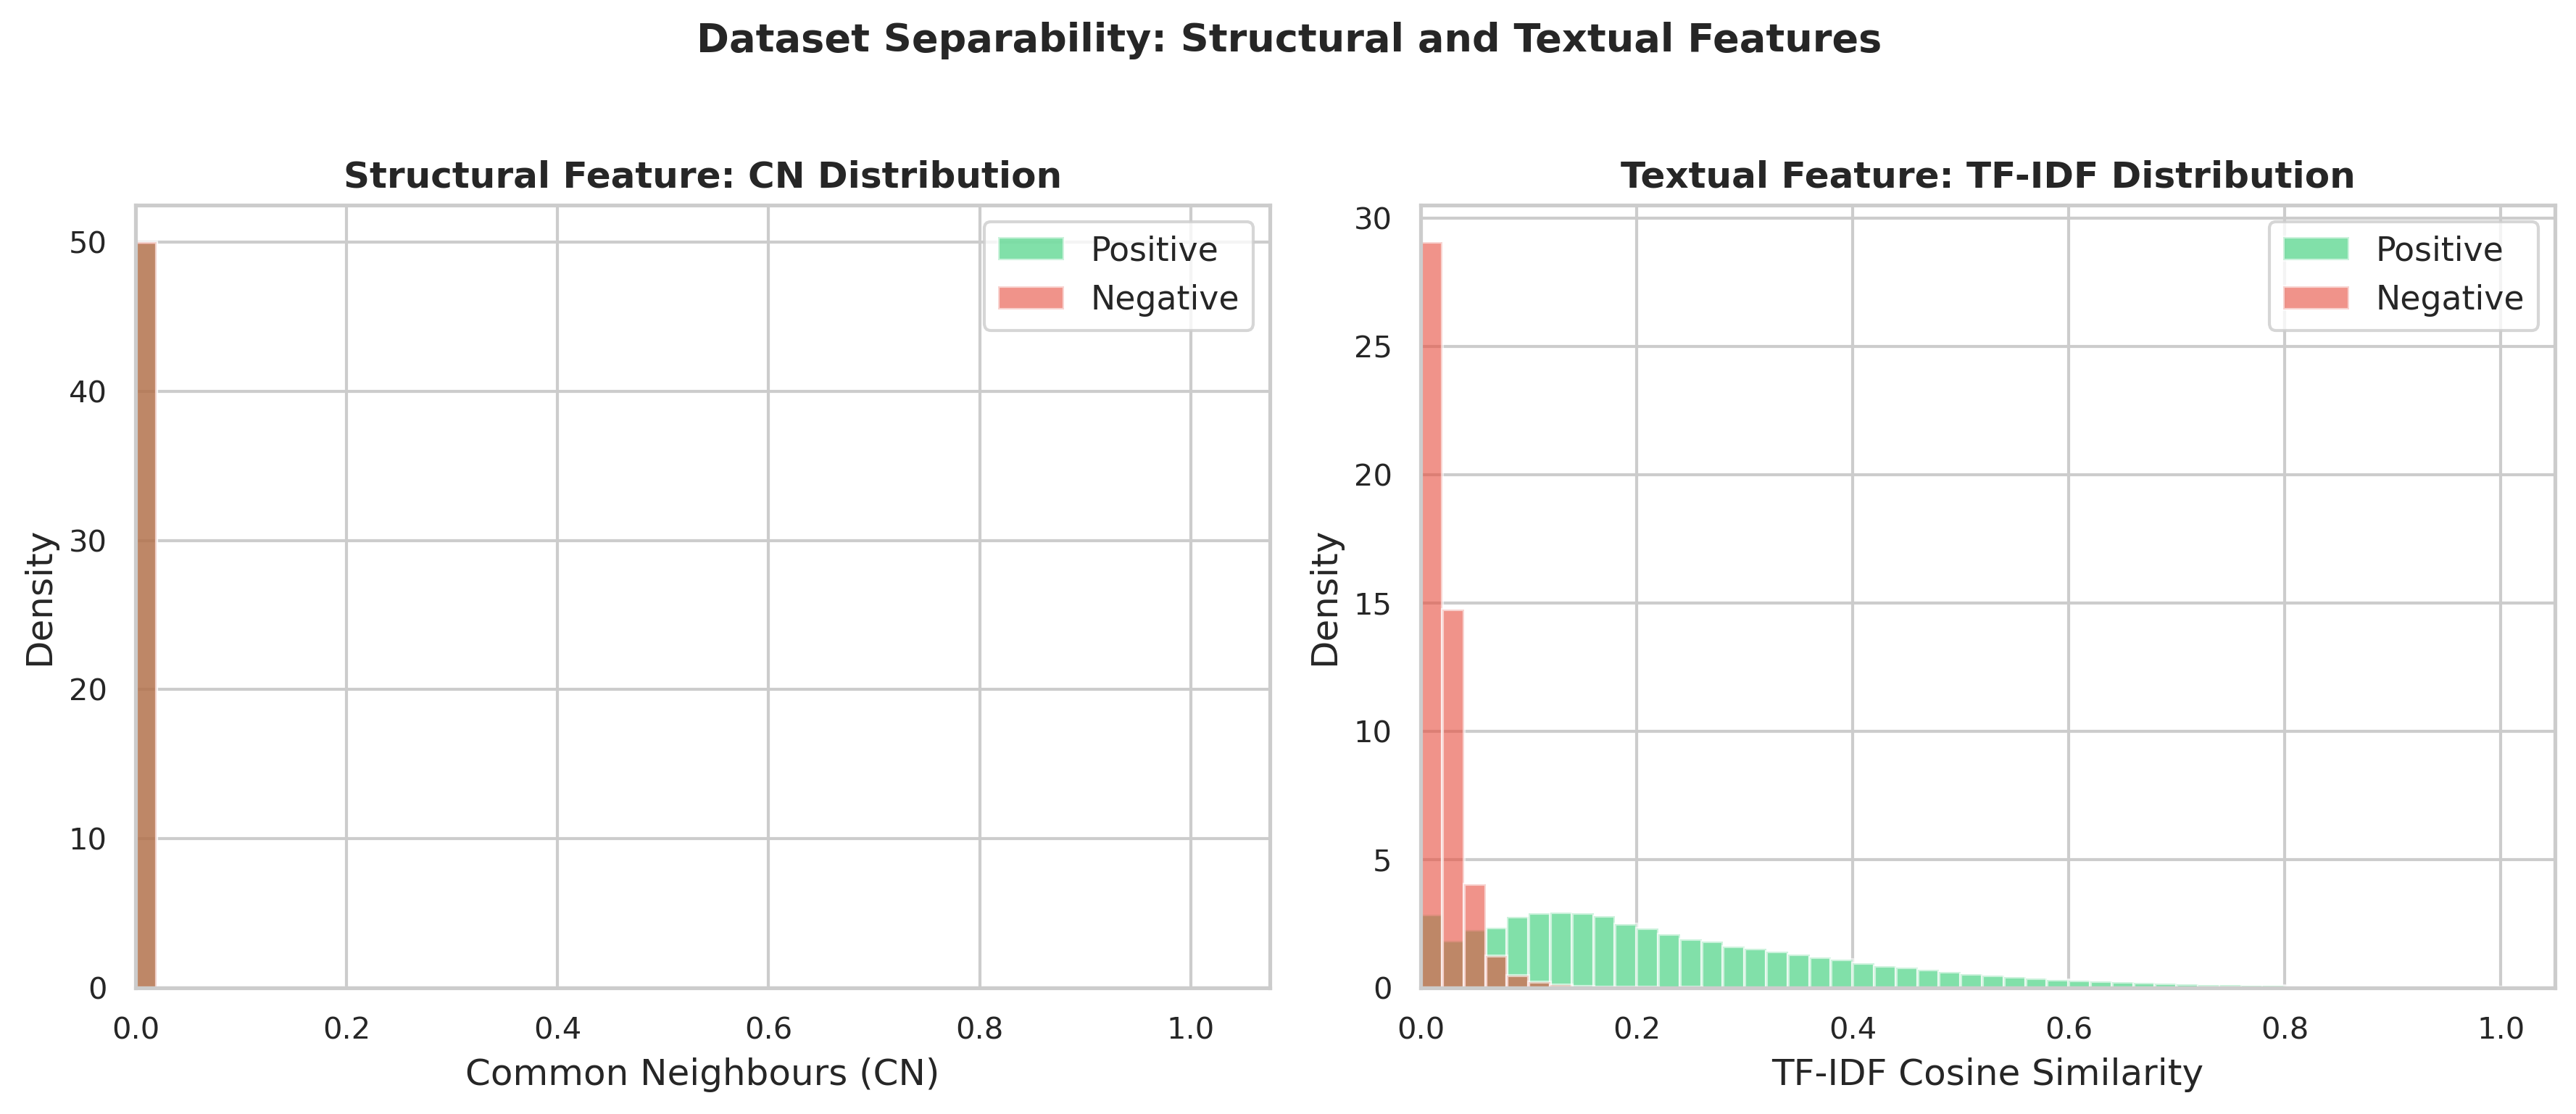
\includegraphics[width=0.9\textwidth]{separability_distributions}
  \caption{Κατανομές Κοινών Γειτόνων και ομοιότητας \en{TF-IDF} για θετικά και αρνητικά ζεύγη (χωρίς αυτοβρόχους). Η καθαρή διαχωρισιμότητα της \en{TF-IDF} υποδηλώνει ότι το κειμενικό περιεχόμενο παρέχει ισχυρό σήμα.}
  \label{fig:separability-dist}
\end{figure}

\begin{figure}[h!]
  \centering
  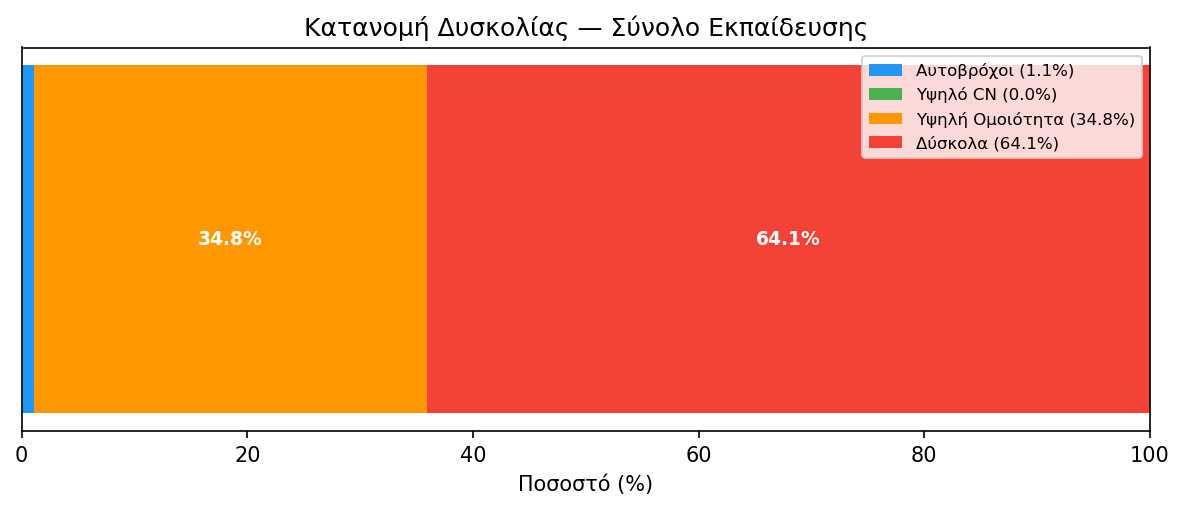
\includegraphics[width=0.7\textwidth]{difficulty_breakdown}
  \caption{Κατανομή της λειτουργικής ετικέτας δυσκολίας στο σύνολο εκπαίδευσης. Η κατηγορία «δύσκολο» δηλώνει ότι δεν ικανοποιείται κανένα από τα τρία απλά κριτήρια.}
  \label{fig:difficulty-breakdown}
\end{figure}

Τα αποτελέσματα δείχνουν ότι το \TrainDiffHardPct\% του συνόλου δεδομένων δεν
ικανοποιεί κανένα από τα τρία απλά κριτήρια, ενώ το \TrainDiffTrivialPct\%
ικανοποιεί τουλάχιστον ένα. Η ονομασία «δύσκολο» είναι λειτουργική και δεν
αποδεικνύει ότι το ζεύγος απαιτεί σημασιολογική συλλογιστική· το τεχνούργημα της
\S\ref{sec:hub-artifact} δείχνει ότι μπορεί να υπάρχει άλλο, μη σχεσιακό σήμα.


\section{Αποτελέσματα \en{CascadeLP} ανά Επίπεδο και Δυσκολία}
\label{sec:cascade-results}

Εκπαιδεύουμε τα τρία επίπεδα ταξινομητών του \en{CascadeLP} αποκλειστικά στο 80\% του
συνόλου εκπαίδευσης (\TrainSplitSize{} ζεύγη, εξαιρουμένων των αυτοβρόχων) και αξιολογούμε σε ένα
παρακρατημένο, στρωματοποιημένο σύνολο επικύρωσης \ValSplitSize{} ζευγών που δεν συμμετέχει
στην εκπαίδευση κανενός ταξινομητή, αλλά έχει επηρεάσει την κατασκευή του
δομικού γραφήματος όπως περιγράφεται στη \S\ref{subsec:data-splits}.
Στα προεπιλεγμένα όρια αξιοπιστίας ($\tau_1 = \TauOneDefault$,
$\tau_2 = \TauTwoDefault$· βλ.\ \S\ref{sec:ablation} για την ευαισθησία ως προς αυτή την επιλογή),
το μοντέλο επιτυγχάνει \en{Macro F1} = \CascadeValFone{} και \en{AUC-ROC} = \CascadeValAuc{} στο σύνολο
επικύρωσης.
Η αυτόνομη βασική γραμμή \en{POS} πετυχαίνει ελαφρώς υψηλότερο \en{Macro F1}
(0{,}9988 έναντι 0{,}9986). Επομένως το αποτέλεσμα του \en{DSAA} δεν δείχνει
βελτίωση του \en{CascadeLP} έναντι κάθε επιμέρους μοντέλου· δείχνει κυρίως ότι
πολλές διαφορετικές μέθοδοι κορεστούν στο ίδιο προβληματικό πεδίο αξιολόγησης.

\begin{table}[h!]
  \centering
  \begin{tabular}{lrrcc}
    \toprule
    \textbf{Επίπεδο} & \textbf{n} & \textbf{Δρομολόγηση} & \textbf{Ακρίβεια} & \textbf{\en{Macro F1}} \\
    \midrule
    Επίπεδο~0 (αυτοβρόχος)      & 0       & 0{,}00\%  & --     & --     \\
    Επίπεδο~1 (\en{Structural}) & \TierOneCount{} & \TierOnePct\% & \TierOneAcc{} & \TierOneFone{} \\
    Επίπεδο~2 (\en{POS + RF})   & \TierTwoCount{} & \TierTwoPct\% & \TierTwoAcc{} & \TierTwoFone{} \\
    Επίπεδο~3 (\en{Embedding})  & \TierThreeCount{} & \TierThreePct\% & \TierThreeAcc{} & \TierThreeFone{} \\
    \bottomrule
  \end{tabular}
  \caption{Ποσοστό δρομολόγησης και απόδοση ανά επίπεδο στο σύνολο επικύρωσης (n=\ValSplitSize{}).}
  \label{tab:cascade-tier-results}
\end{table}

Ο πίνακας~\ref{tab:cascade-tier-results} αποκαλύπτει δύο ευρήματα που δεν προκύπτουν από
τη συνολική βαθμολογία.
Πρώτον, το Επίπεδο~1 έχει ακρίβεια \TierOneAcc{} αλλά \en{Macro F1}
μόλις \TierOneFone --- πρακτικά τυχαία απόδοση παρά την υψηλή ακρίβεια.
Η αιτία είναι η
ακραία ανισορροπία κλάσεων μέσα στο υποσύνολο ζευγών για τα οποία ο
\texttt{\en{StructuralClassifier}} δηλώνει αξιοπιστία $\geq \tau_1$: το \TierOnePosPct\% αυτών
των ζευγών είναι θετικό, και ο ταξινομητής προβλέπει θετική ετικέτα στο 100\% των
περιπτώσεων, χωρίς καμία πρόβλεψη αρνητικής ετικέτας.
Το αποτέλεσμα είναι μηδενική
ανάκληση για την σπάνια αρνητική κλάση, ακριβώς το σενάριο για το οποίο επιλέχθηκε το
\en{Macro F1} ως πρωτεύουσα μετρική (Κεφάλαιο~\ref{ch:experiments}) αντί της απλής
ακρίβειας.
Δεύτερον, το Επίπεδο~3 --- τα \TierThreeCount{} ζεύγη (\TierThreePct\%) που κλιμακώνονται μέχρι τον
\texttt{\en{EmbeddingClassifier}} --- έχει ακρίβεια μόλις \TierThreeAcc.
Η κατεύθυνση του
σφάλματος είναι επίσης ασύμμετρη: οι πραγματικές ετικέτες είναι \TierThreeTruePosPct\% θετικές, ενώ οι
προβλέψεις είναι μόλις \TierThreePredPosPct\% θετικές.
Η ασυμμετρία αυτή αποκαλύπτει συστηματική
μεροληψία: ο ταξινομητής \en{Embedding} τείνει προς υποπρόβλεψη θετικής ετικέτας σε αυτό
το συγκεκριμένο υπόλειμμα ζευγών, που αναλύεται περαιτέρω στη \S\ref{sec:hard-residual}.

Ο πίνακας διασταύρωσης επιπέδου$\times$δυσκολίας (πίνακας~\ref{tab:cascade-tier-difficulty})
δείχνει ότι τα σφάλματα του Επιπέδου~1 και του Επιπέδου~3 συγκεντρώνονται στην κατηγορία
\en{hard}: το Επίπεδο~1 έχει ακρίβεια \TierOneHardAcc{} στα \TierOneHardN{} δύσκολα ζεύγη που χειρίζεται
έναντι \TierOneHighTextsimAcc{} στα τετριμμένα ζεύγη υψηλής ομοιότητας κειμένου που φτάνουν ως αυτό, και το
Επίπεδο~3 καταρρέει στα \TierThreeHardN{} δύσκολα ζεύγη του (ακρίβεια \TierThreeHardAcc) ενώ επιλύει τέλεια τα
υπόλοιπα \TierThreeHighTextsimN{} τετριμμένα ζεύγη που το φτάνουν.
Το Επίπεδο~2 παραμένει σχεδόν αλάνθαστο
(ακρίβεια $\geq$ 0{,}9989) και στις δύο κατηγορίες δυσκολίας, γεγονός που εξηγεί γιατί
χειρίζεται το \TierTwoPct\% του συνόλου επικύρωσης χωρίς να προκαλεί κλιμάκωση.
Από τα \CascadeTotalErrors{}
συνολικά σφάλματα ταξινόμησης στο σύνολο επικύρωσης, το \CascadeErrorsHardPct\% προέρχεται από ζεύγη
που χαρακτηρίζονται \en{hard} και μόλις το \CascadeErrorsTrivialPct\% από τετριμμένα ζεύγη υψηλής ομοιότητας
κειμένου --- τα λάθη του \en{CascadeLP} συγκεντρώνονται σχεδόν αποκλειστικά στο υποσύνολο
που το πρωτόκολλο χαρακτηρισμού δυσκολίας (\S\ref{sec:forensics-protocol}) είχε ήδη
προσδιορίσει ως μη διαχωρίσιμο από τα απλά κριτήρια.

\begin{table}[h!]
  \centering
  \small
  \begin{tabular}{lrrr}
    \toprule
    \textbf{Επίπεδο} & \textbf{\en{hard}} & \textbf{Υψηλό \en{CN}} & \textbf{Υψηλή Ομοιότητα Κειμένου} \\
    \midrule
    Επίπεδο~1 & n=\TierOneHardN, \TierOneHardAcc{} & n=\TierOneHighCnN, 1{,}0 & n=\TierOneHighTextsimN, 1{,}0 \\
    Επίπεδο~2 & n=\TierTwoHardN, \TierTwoHardAcc{} & ---         & n=\TierTwoHighTextsimN, \TierTwoHighTextsimAcc{} \\
    Επίπεδο~3 & n=\TierThreeHardN, \TierThreeHardAcc{} & ---         & n=\TierThreeHighTextsimN, 1{,}0 \\
    \bottomrule
  \end{tabular}
  \caption{Πίνακας διασταύρωσης επιπέδου$\times$δυσκολίας: πλήθος ζευγών και ακρίβεια ανά
  συνδυασμό, σύνολο επικύρωσης.}
  \label{tab:cascade-tier-difficulty}
\end{table}

Στο σύνολο ελέγχου, όπου δεν υπάρχουν πραγματικές ετικέτες στα δεδομένα μας και άρα
μετράμε τοπικά μόνο ποσοστά κλήσεων ανά επίπεδο, παρατηρούμε μια αξιοσημείωτη μετατόπιση
σε σχέση με το σύνολο επικύρωσης: το Επίπεδο~1 χειρίζεται μόλις το \TestTierOnePct\% των ζευγών
ελέγχου (\TestTierOneCount{} από \TestPairs{}) έναντι \TierOnePct\% στο σύνολο επικύρωσης, με το Επίπεδο~2 να
απορροφά την υπόλοιπη κίνηση στο \TestTierTwoPct\%.
Το Επίπεδο~0 χειρίζεται \SelfLoopsTest{} ζεύγη (\TestTierZeroPct\%)
--- αριθμός που ταυτίζεται ακριβώς με το πλήθος αυτοβρόχων που καταγράφηκε στον έλεγχο
\en{data leakage} (\S\ref{sec:leakage-results}), λειτουργώντας ως ανεξάρτητος έλεγχος
ορθότητας της διαδρομής δρομολόγησης.
Η μετατόπιση στο Επίπεδο~1 δεν είναι σφάλμα
υλοποίησης, αλλά άμεση συνέπεια του τρόπου κατασκευής του δομικού γραφήματος: το γράφημα
περιλαμβάνει αποκλειστικά τις θετικές ακμές του συνόλου \textit{εκπαίδευσης}
(\S\ref{sec:cascade-routing}), οπότε και οι δύο κόμβοι ενός ζεύγους εμφανίζονται σε αυτό
για το \GraphCoverageTrainPct\% των ζευγών εκπαίδευσης/επικύρωσης, αλλά μόλις για το \GraphCoverageTestPct\% των ζευγών
ελέγχου.
Τα ζεύγη ελέγχου είναι δηλαδή δομικά πιο «ψυχρά» από τα ζεύγη επικύρωσης, το
Επίπεδο~1 στερείται σήματος γι' αυτά και η δρομολόγηση κλιμακώνει σχεδόν αυτόματα στο
Επίπεδο~2.
Η ανάλυση της απόδοσης ειδικά στο υποσύνολο μηδενικού \en{CN}
αναλαμβάνεται στη \S\ref{sec:cold-start-results}.

Παρότι το \en{DSAA 2023} δεν δημοσιεύει τις πραγματικές ετικέτες του συνόλου ελέγχου,
ο διαγωνισμός διατηρεί ενεργό πίνακα κατάταξης στο \en{Kaggle} που βαθμολογεί
υποβληθείσες προβλέψεις.
Υποβάλλοντας τις προβλέψεις του \en{CascadeLP} στο σύνολο
ελέγχου (\texttt{\en{outputs\slash{}predictions\slash{}cascade\_submission.csv}}) λάβαμε δημόσια
βαθμολογία \en{Macro F1} = \KaggleBaselinePublic{}. Η συμφωνία με τη βαθμολογία
επικύρωσης (\CascadeValFone{}) δείχνει ότι το ίδιο μοτίβο είναι παρόν και στο
κρυφό σύνολο ελέγχου, αλλά δεν διαχωρίζει τη σχεσιακή πρόβλεψη από την αξιοποίηση
του τεχνουργήματος δειγματοληψίας της \S\ref{sec:hub-artifact}.


\section{Αποτελέσματα στο Ανεξάρτητο Σύνολο \en{Wikipedia}}
\label{sec:wiki-fresh}
\label{subsec:wiki-fresh-results}

Στο δεύτερο σύνολο επανεκπαιδεύουμε από την αρχή την ίδια διαμόρφωση του
\en{CascadeLP}, χωρίς αλλαγή αρχιτεκτονικής ή ορίων, και αξιολογούμε τους ίδιους
πέντε αυτόνομους ταξινομητές. Τα αποτελέσματα παρουσιάζονται στον
Πίνακα~\ref{tab:wiki-fresh-results}.

\begin{table}[h!]
  \centering
  \begin{tabular}{lrr}
    \toprule
    \textbf{Μοντέλο} & \textbf{\en{Macro F1}} & \textbf{\en{AUC-ROC}} \\
    \midrule
    Δομικό (\en{CN/Jaccard/AA/PA})       & \WfStructuralFone{} & \WfStructuralAuc{} \\
    \en{TF-IDF + Λογιστική Παλινδρόμηση} & \WfTfidfFone{}      & \WfTfidfAuc{} \\
    \en{POS + Random Forest}             & \WfPosFone{}        & \WfPosAuc{} \\
    Ομοιότητα \en{Sentence-Transformer}  & \WfEmbeddingFone{}  & \WfEmbeddingAuc{} \\
    \en{TF-IDF + SVM}                    & \WfSvmFone{}        & \WfSvmAuc{} \\
    \en{CascadeLP}                       & \textbf{\WfCascadeFone{}} & \textbf{\WfCascadeAuc{}} \\
    \bottomrule
  \end{tabular}
  \caption{Αποτελέσματα στο ανεξάρτητο σύνολο Απλής Αγγλικής \en{Wikipedia}
  (n=\WfValSplitSize{} ζεύγη επικύρωσης). Όλα τα μοντέλα επανεκπαιδεύονται από
  την αρχή χωρίς αλλαγή της αρχιτεκτονικής ή των υπερπαραμέτρων τους.}
  \label{tab:wiki-fresh-results}
\end{table}

Το \en{CascadeLP} πετυχαίνει \en{Macro F1} = \WfCascadeFone{}, υψηλότερο από
κάθε μεμονωμένη οικογένεια χαρακτηριστικών. Ο δομικός ταξινομητής είναι η
ισχυρότερη αυτόνομη οικογένεια με \WfStructuralFone{}, γεγονός που επιβεβαιώνει
ότι το πυκνότερο γράφημα παρέχει χρήσιμο σχεσιακό σήμα. Η δρομολόγηση ακολουθεί
επίσης τον σχεδιαστικό στόχο: το Επίπεδο~1 επιλύει \WfTierOneCount{} ζεύγη
(\WfTierOnePct\%), το Επίπεδο~2 \WfTierTwoCount{} (\WfTierTwoPct\%) και το
Επίπεδο~3 \WfTierThreeCount{} (\WfTierThreePct\%). Τα ποσοστά αυτά μετρούν ποιο
επίπεδο έλαβε την τελική απόφαση πάνω σε προϋπολογισμένα χαρακτηριστικά· δεν
αποτελούν μέτρηση ίσης ποσοστιαίας μείωσης του κόστους κωδικοποίησης.


\section{Σύγκριση με Μοντέλο Αναφοράς \en{SVM}}
\label{sec:svm-results}

Ως μοντέλο αναφοράς εκπαιδεύουμε έναν ταξινομητή \en{TF-IDF + SVM} (RBF kernel SVC
σε ένα στρωματοποιημένο υποσύνολο \SvmSampleSize{} ζευγών για να αποφύγουμε το τετραγωνικό υπολογιστικό κόστος
σε 948K ζεύγη). Σημειώνεται ότι ο περιορισμός του μεγέθους εκπαίδευσης είναι εσκεμμένη
επιλογή λόγω του απαγορευτικού κόστους του αλγορίθμου. Συνεπώς, η σύγκριση με τα 
άλλα μοντέλα γίνεται με άξονα τον λόγο κόστους-απόδοσης σε ένα πρακτικά
εφικτό σενάριο εκπαίδευσης, και δεν αντικατοπτρίζει απαραίτητα τη μέγιστη
θεωρητική ικανότητα της μεθόδου \en{SVM}.
Τα αποτελέσματα επικύρωσης είναι:

\begin{table}[h!]
  \centering
  \begin{tabular}{lcc}
    \toprule
    \textbf{Μέτρο} & \textbf{Τιμή} \\
    \midrule
    \en{Macro F1-score} & \SvmFone{} \\
    \en{AUC-ROC} & \SvmAuc{} \\
    \en{Macro F1} μηδενικού \en{CN} & \SvmCsFone{} \\
    Καθυστέρηση & \SvmLatency{} ms/ζεύγος \\
    \bottomrule
  \end{tabular}
  \caption{\en{SVM} αποτελέσματα επικύρωσης σε \ValSplitSize{} ζεύγη.}
  \label{tab:svm-results}
\end{table}

\begin{figure}[h!]
  \centering
  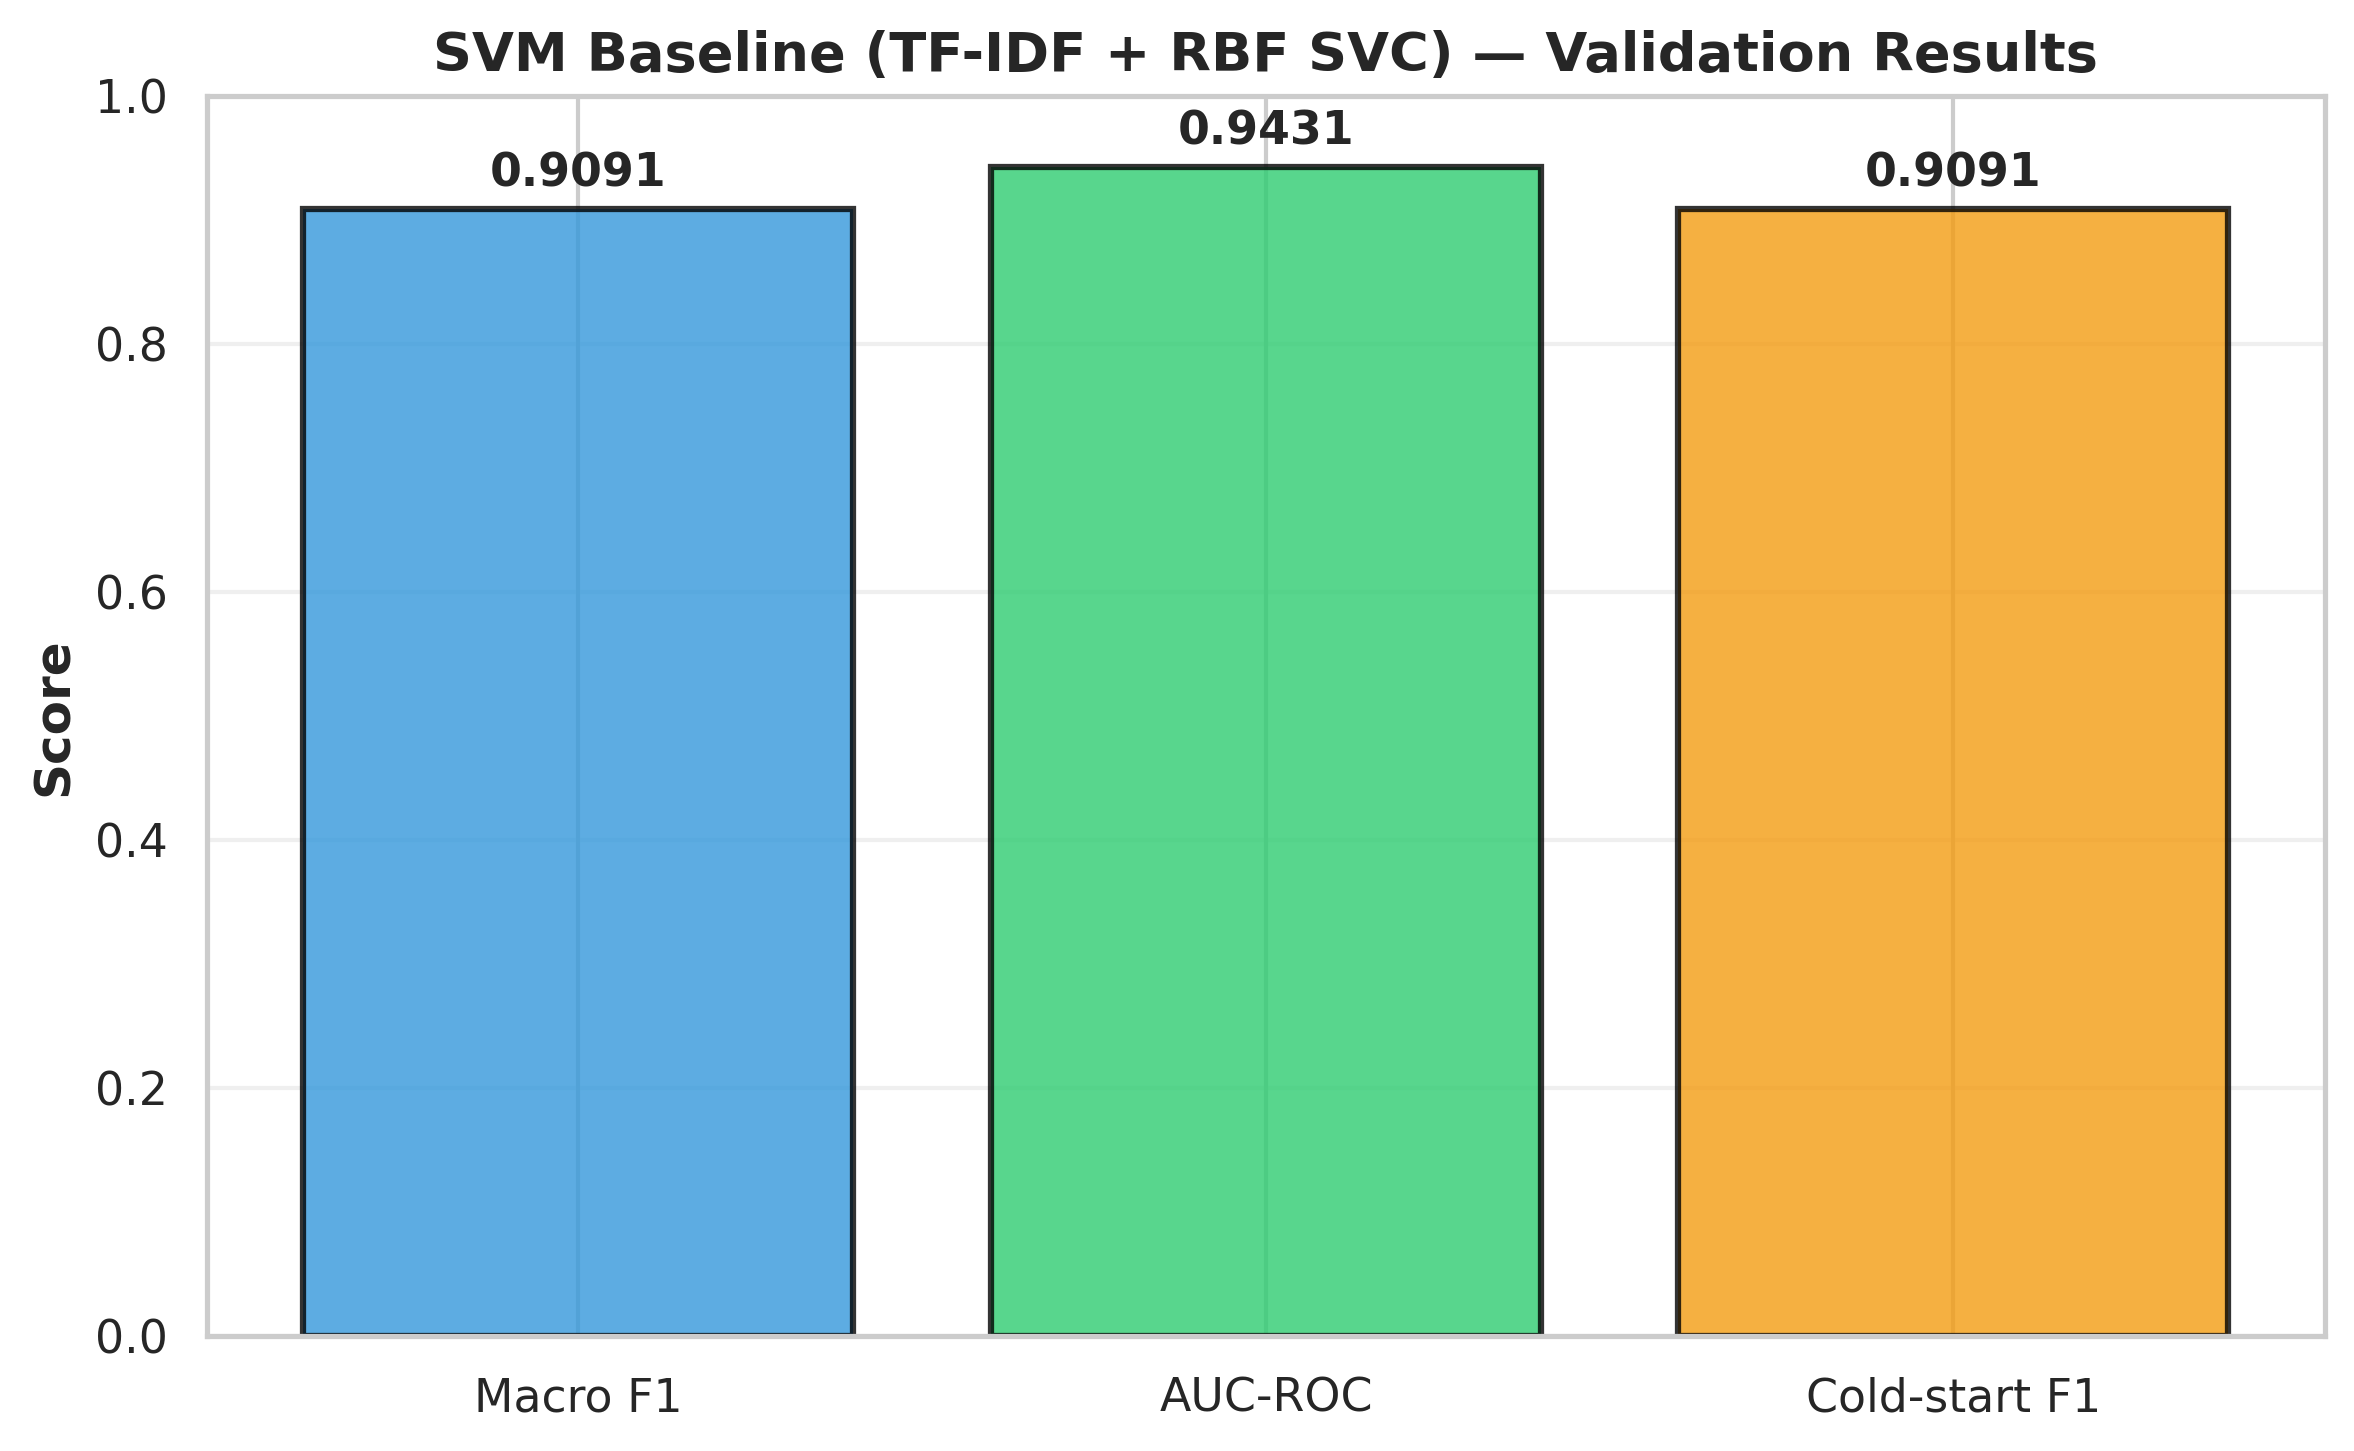
\includegraphics[width=0.8\textwidth]{svm_metrics}
  \caption{Απόδοση μοντέλου αναφοράς \en{TF-IDF + SVM} σε σύνολο επικύρωσης. Το \en{SVM} επιτυγχάνει \en{Macro F1} = \SvmFone{} και \en{AUC-ROC} = \SvmAuc{}, υποδηλώνοντας την ισχυρή προβλεπτική ικανότητα της κειμενικής ομοιότητας.}
  \label{fig:svm-metrics}
\end{figure}

Το \en{SVM} επιτυγχάνει υψηλή απόδοση σε όλες τις μετρικές, υπογραμμίζοντας ότι η
\en{TF-IDF} ομοιότητα του κειμένου είναι ένας ισχυρός μεμονωμένος δείκτης για τη
πρόβλεψη ακμών σε αυτό το σύνολο δεδομένων.
Η σύγκριση με τη \en{CascadeLP}
θα δείξει κατά πόσον οι πολυστοιχειακές δομικές και σημασιολογικές προσεγγίσεις
παρέχουν περαιτέρω κέρδη απόδοσης ή απλώς αναδημιουργούν τα αποτελέσματα που
καταδεικνύονται ήδη από τη \en{TF-IDF}.
                % Ch.4 Πειράματα             \ref{chap:experiments}
    % Chapter 5: Analysis — ablation, cold-start, hard-residual, efficiency, error analysis
\selectlanguage{greek}


\chapter{Ανάλυση}
\label{ch:analysis}

\section{Στρέβλωση στη Δειγματοληψία Αρνητικών Παραδειγμάτων}
\label{sec:hub-artifact}

Η βαθμολογία \en{Macro F1} = \CascadeValFone{} του \en{CascadeLP}
(\S\ref{sec:cascade-results}) δεν εξηγείται από απλή επικάλυψη ζευγών
εκπαίδευσης και ελέγχου (\S\ref{sec:leakage-results}). Αυτός ο έλεγχος όμως
δεν καλύπτει στρεβλώσεις στη διαδικασία δειγματοληψίας ούτε τη διαρροή
δομικής πληροφορίας από την κατασκευή του γραφήματος πριν από τη διαίρεση
(\S\ref{subsec:data-splits}). Μια βαθμολογία τόσο κοντά στο τέλειο σε ένα πρόβλημα διμελούς
ταξινόμησης 948 χιλιάδων ζευγών αξίζει έναν επιπλέον, ανεξάρτητο έλεγχο: πόσο
από αυτή την ακρίβεια θα μπορούσε να αναπαραχθεί χωρίς καμία σχεσιακή ή
σημασιολογική πληροφορία;

Ομαδοποιώντας τις μη αυτοαναφορικές γραμμές του \texttt{\en{train.csv}} ανά
τιμή του πρώτου άκρου \texttt{\en{id1}}, βρίσκουμε ότι από \HubUniqueSourceCount{}
μοναδικές τιμές, ακριβώς \HubCount{} εμφανίζονται τουλάχιστον \HubThreshold{}
φορές η καθεμία---το ίδιο σύνολο τιμών προκύπτει και σε όρια 50 και 200, οπότε
το εύρημα δεν εξαρτάται από την ακριβή επιλογή ορίου.
Αυτοί οι \HubCount{}
«κόμβοι-συγκέντρωσης» αντιστοιχούν σε \HubRowCount{} γραμμές (\HubRowPct\% του
συνόλου) και είναι \HubPurityPct\% αρνητικοί.
Κάθε άλλη γραμμή---\NonHubRowCount{}
γραμμές---είναι θετική με ακρίβεια \NonHubPosPct\%.
Ένας ταξινομητής
αναζήτησης---πρόβλεψη της πλειοψηφικής ετικέτας του κόμβου-συγκέντρωσης όταν
το \texttt{\en{id1}} ανήκει σε αυτούς τους \HubCount{}, αλλιώς πρόβλεψη θετικής
ετικέτας---χωρίς κείμενο, γράφημα, ή εκπαίδευση μοντέλου, πετυχαίνει
\en{Macro F1} = \HubLookupFone{} και ακρίβεια \HubLookupAcc{} σε ολόκληρο το
\texttt{\en{train.csv}}.
Και οι \HubTestOverlap{} τιμές εμφανίζονται στο
\texttt{\en{test.csv}}, καλύπτοντας το \HubTestRowPct\% των γραμμών ελέγχου---
η ίδια συντόμευση είναι επομένως διαθέσιμη και στο πραγματικό σύνολο ελέγχου
και στον δημόσιο πίνακα κατάταξης του διαγωνισμού.

\begin{figure}[htbp]
  \centering
  \includegraphics[width=\textwidth]{negative_sampling_artifact}
  \caption{Η στρέβλωση στη δειγματοληψία αρνητικών παραδειγμάτων στο \en{DSAA 2023}. Οι
  \HubCount{} συχνές τιμές του πρώτου άκρου είναι σχεδόν αποκλειστικά
  αρνητικές, ενώ όλες οι υπόλοιπες είναι θετικές, και το ίδιο σύνολο πηγών
  καλύπτει παρόμοιο ποσοστό του αρχείου ελέγχου. Ο κανόνας αναζήτησης μόνο από
  την ταυτότητα του πρώτου άκρου πετυχαίνει \en{Macro F1} =
  \HubLookupFone{}.}
  \label{fig:negative-sampling-artifact}
\end{figure}

Ένα μόνο παράδειγμα καθιστά το φαινόμενο απτό.
Το άρθρο \en{«2016 Chinese FA
Women's Super Cup»} (ένα ποδοσφαιρικό κύπελλο) είναι κόμβος-συγκέντρωσης,
συζευγμένο στο σύνολο εκπαίδευσης με εκατοντάδες ουσιαστικά τυχαίους στόχους,
όλους με αρνητική ετικέτα: το έντομο \en{«E. placida»}, τον ηθοποιό \en{«Frank
Jude Jr.»}, τον αστρονόμο του 17ου αιώνα \en{«Francesco Stelluti»}, το
αεροδρόμιο \en{«Omaka Aerodrome»}, και άλλους.
Καμία θεματική, γεωγραφική, ή
χρονική σχέση δεν συνδέει κανένα από αυτά τα ζεύγη με το άρθρο του κυπέλλου---
πρόκειται ορατά για έναν κόμβο-πηγή συζευγμένο με ένα αυθαίρετο δείγμα του
σώματος κειμένων, όχι για μια επιμελημένη συλλογή εύλογων μη-συνδέσμων.
Ο
πληθυσμός εκτός κόμβων-συγκέντρωσης έχει διάμεσο πλήθος μίας γραμμής ανά τιμή
\texttt{\en{id1}} και σχεδόν καθολική θετική ετικέτα---συνεπές με δείγμα
γνήσιων υπερσυνδέσμων.
Ο πληθυσμός των κόμβων-συγκέντρωσης έχει έως και
$\sim$8.000 γραμμές ανά τιμή---συνεπές με μαζική δειγματοληψία αρνητικών
παραδειγμάτων γύρω από έναν μικρό αριθμό αυθαίρετων άρθρων-αγκυρών.

\subsection{Το Τεχνούργημα «εν Δράσει»}
\label{subsec:hub-in-action}

Το παραπάνω εύρημα αφορά το σύνολο δεδομένων καθαυτό.
Για να δείξουμε ότι
επηρεάζει και το πραγματικό, ήδη αναφερόμενο μοντέλο, διασταυρώνουμε το
σύνολο των \HubCount{} κόμβων-συγκέντρωσης απευθείας με τις υπαρκτές
προβλέψεις του \en{CascadeLP} στο σύνολο επικύρωσης
(\texttt{\en{outputs\slash{}predictions\slash{}cascade\_val\_tiers.csv}},
χωρίς καμία επανεκπαίδευση ή αλλαγή πρωτοκόλλου).
Το \HubValSourcedPct\% των
\ValSplitSize{} ζευγών επικύρωσης έχει κόμβο-συγκέντρωσης ως πρώτο άκρο· ένας
απλός πίνακας αναζήτησης πάνω σε αυτό ακριβώς το υποσύνολο ζευγών πετυχαίνει
\en{Macro F1} = \HubValLookupFone{}.
Ο κανόνας ορίζεται περιγραφικά από το πλήρες επισημασμένο αρχείο και επομένως
δεν αποτελεί ανεξάρτητα εκπαιδευμένο μοντέλο αναφοράς.
Χρησιμοποιείται ως
διαγνωστικός έλεγχος του πόσο άμεσα κωδικοποιείται η ετικέτα στην ταυτότητα
του πρώτου άκρου.
Πιο αποκαλυπτικό: οι προβλέψεις του πραγματικού, εκπαιδευμένου
\en{CascadeLP} συμφωνούν με τον τετριμμένο πίνακα αναζήτησης στο
\HubValAgreementPct\% όλων των ζευγών επικύρωσης, και στο
\HubValHubAgreementPct\% των ζευγών με κόμβο-συγκέντρωσης.
Το εκπαιδευμένο
μοντέλο, δηλαδή, δεν διαφέρει σχεδόν καθόλου από τον απλό κανόνα «είναι το
\texttt{\en{id1}} ένας από αυτούς τους \HubCount{} κόμβους;» σε πάνω από τα
μισά ζεύγη του συνόλου επικύρωσης.

Αυτό δεν σημαίνει ότι το \en{CascadeLP} είναι λανθασμένο ως αρχιτεκτονική---
δρομολογεί σωστά και κλιμακώνει με βάση την αξιοπιστία των υποκείμενων
χαρακτηριστικών, όπως σχεδιάστηκε.
Σημαίνει ότι το συγκεκριμένο σύνολο
δεδομένων \en{DSAA 2023} δεν επιτρέπει να διακρίνουμε «το \en{CascadeLP}
έμαθε να προβλέπει υπερσυνδέσμους» από «το \en{CascadeLP} έμαθε να αναγνωρίζει
\HubCount{} συγκεκριμένους κόμβους»---και οι δύο υποθέσεις προβλέπουν σχεδόν
πανομοιότυπα αποτελέσματα σε αυτό το σύνολο δεδομένων.
Η ίδια ασάφεια πλήττει
πιθανότατα και κάθε άλλη αναφερόμενη σχεδόν τέλεια βαθμολογία σε αυτό το
σύνολο δεδομένων, συμπεριλαμβανομένων προηγούμενων υποβολών του διαγωνισμού
που βασίζονται σε χαρακτηριστικά \en{POS} (Κεφάλαιο~\ref{ch:background}): καμία
δεν αναφέρει έλεγχο ανάλογο του παρόντος.
Η \S\ref{sec:wiki-fresh} απαντά στο
ερώτημα που αφήνει ανοιχτό αυτή η ασάφεια, εκπαιδεύοντας από την αρχή την ίδια
αρχιτεκτονική \en{CascadeLP} σε ένα σύνολο δεδομένων του οποίου η διαδικασία τυχαίας
δειγματοληψίας αρνητικών αποφεύγει τη συγκεκριμένη συγκέντρωση πηγών.

Η υψηλή απόδοση του \texttt{\en{PosClassifier}} στο \en{DSAA 2023}
(\en{Macro F1} = \TierTwoFone{} ως αυτόνομο μοντέλο αναφοράς,
\S\ref{sec:cascade-results}, χειριζόμενο το \TierTwoPct\% του συνόλου
επικύρωσης) χρειάζεται την ίδια επιφύλαξη με τη συνολική βαθμολογία του
\en{CascadeLP}.
Ένα \en{Random Forest} πάνω σε συχνότητες μερών του λόγου δεν
έχει προφανή λόγο να αναγνωρίζει την ύπαρξη υπερσυνδέσμου με τέτοια ακρίβεια·
όμως αν οι κόμβοι-συγκέντρωσης του \texttt{\en{id1}} έχουν συστηματικά
διαφορετικό ύφος κειμένου (π.χ. άρθρα αθλητικών διοργανώσεων, όπως στο
παράδειγμα \en{«2016 Chinese FA Women's Super Cup»} παραπάνω) από τον
πληθυσμό-στόχο με τον οποίο συζευγνύονται, το διάνυσμα \en{POS} μπορεί να
«αναγνωρίζει» τον χαρακτηριστικό κόμβο-πηγή, όχι τη σχέση μεταξύ των δύο
άκρων --- η ίδια στρέβλωση σε διαφορετική οικογένεια
χαρακτηριστικών.
Η σχεδόν τέλεια βαθμολογία δεν αποδεικνύει άρα ότι το μοντέλο
έμαθε μια γνήσια σχέση μεταξύ δύο άρθρων· είναι ακριβώς αυτό που θα αναμενόταν
αν το μοντέλο εκμεταλλεύεται τη στρέβλωση στη δειγματοληψία.
Η αντίστιξη με το
ανεξάρτητο σύνολο Απλής Αγγλικής \en{Wikipedia} είναι εδώ κατατοπιστική: υπό
την ίδια αρχιτεκτονική και τις ίδιες προεπιλεγμένες υπερπαράμετρους, ο
αυτόνομος \texttt{\en{PosClassifier}} πέφτει σε \en{Macro F1} = \WfPosFone{}
(\S\ref{sec:wiki-fresh}), και η κατάταξη των οικογενειών χαρακτηριστικών
αλλάζει ουσιωδώς --- συνεπές με την υπόθεση ότι η επίδοσή του στο \en{DSAA
2023} αντανακλά σε μεγάλο βαθμό αυτή τη στρέβλωση και όχι εγγενή ισχύ της
οικογένειας χαρακτηριστικών \en{POS} καθαυτής.


\section{Ευαισθησία στη Σειρά των Άκρων}
\label{sec:endpoint-swap}

Η ετικέτα-στόχος αυτής της εργασίας είναι συμμετρική ως προς τα δύο άκρα ενός
ζεύγους: $y_{uv} = y_{vu}$ εξ ορισμού (\S\ref{sec:problem-definition}). Ο
\texttt{\en{PosClassifier}} του Επιπέδου~2 όμως συνενώνει τα δύο 36-διάστατα
ιστογράμματα \en{POS} διατηρώντας τη σειρά $[\mathbf{p}_u \,\|\, \mathbf{p}_v]$
αντί να τα συμμετροποιεί (\S\ref{subsec:pos-features}), οπότε τίποτα στην
αρχιτεκτονική δεν εγγυάται ότι η πρόβλεψη παραμένει αναλλοίωτη αν ανταλλαχθούν
τα $u$ και $v$.
Ποσοτικοποιούμε την ευαισθησία αυτή αντιστρέφοντας κάθε ζεύγος
του συνόλου επικύρωσης --- εναλλάσσοντας τα δύο μπλοκ χαρακτηριστικών \en{POS}
και τα αντίστοιχα πεδία \texttt{\en{id1}}/\texttt{\en{id2}}, διατηρώντας
αμετάβλητα τα συμμετρικά δομικά και \en{Sentence-Transformer} χαρακτηριστικά
--- και τροφοδοτώντας το ζεύγος στο ήδη εκπαιδευμένο, αναλλοίωτο
\texttt{\en{cascade.joblib}}, χωρίς καμία επανεκπαίδευση
(\texttt{\en{scripts\slash{}dsaa\slash{}audit\_protocol.py --swap}}). Πριν από
τη σύγκριση, ο έλεγχος επαληθεύει ότι οι προβλέψεις και οι δρομολογήσεις πάνω
στα μη-αντεστραμμένα ζεύγη αναπαράγουν επακριβώς το αποθηκευμένο
\texttt{\en{cascade\_val\_tiers.csv}} (\S\ref{subsec:implementation-architecture}),
ώστε η σύγκριση να αφορά πράγματι το ίδιο μοντέλο και το ίδιο σύνολο.

Σε \SwapN{} ζεύγη επικύρωσης, η αντιστροφή αλλάζει την τελική πρόβλεψη του
\en{CascadeLP} στο \SwapLabelChangePct\% των περιπτώσεων, με μέση απόλυτη
μεταβολή πιθανότητας \SwapMeanAbsProbChange{} και αλλαγή του επιπέδου που
αποφασίζει σε \SwapTierChanges{} ζεύγη.
Η επίδραση είναι έντονα ασύμμετρη ως
προς την αρχική ετικέτα: στα ζεύγη με αρχική αρνητική ετικέτα η αντιστροφή
αλλάζει την πρόβλεψη στο \SwapNegClassChangePct\% των περιπτώσεων, ενώ στα
ζεύγη με αρχική θετική ετικέτα μόλις στο \SwapPosClassChangePct\%.
Με άλλα
λόγια, οι προβλέψεις πάνω σε (κατά κανόνα δειγματοληπτημένα) αρνητικά ζεύγη
είναι σχεδόν πάντα ασταθείς ως προς τη σειρά των άκρων, ενώ οι προβλέψεις πάνω
σε γνήσια θετικά ζεύγη παραμένουν σε μεγάλο βαθμό σταθερές.

\begin{figure}[htbp]
  \centering
  \includegraphics[width=0.8\textwidth]{endpoint_swap_sensitivity}
  \caption{Ποσοστό αλλαγής πρόβλεψης μετά την αντιστροφή των άκρων. Η μεγάλη
  διαφορά μεταξύ αρχικά αρνητικών και θετικών ζευγών συνδέει την αστάθεια του
  διατεταγμένου διανύσματος \en{POS} με τη θέση του πρώτου άκρου στο
  \en{DSAA 2023}.}
  \label{fig:endpoint-swap}
\end{figure}

Το εύρημα αυτό \textbf{δεν} τεκμηριώνει ότι το πρόβλημα θα έπρεπε να
αντιμετωπιστεί ως κατευθυνόμενο --- η ετικέτα παραμένει συμμετρική εξ ορισμού
(\S\ref{sec:problem-definition}), και η εργασία δεν αλλάζει τον ορισμό του
προβλήματος με βάση αυτό το εύρημα.
Τεκμηριώνει αντίθετα ένα συγκεκριμένο
περιορισμό \textit{υλοποίησης και αξιολόγησης}: ο \texttt{\en{PosClassifier}}
μπορεί να εκμεταλλεύεται την αυθαίρετη θέση ενός άκρου (ποιο από τα δύο
καταγράφεται ως \texttt{\en{id1}}) αντί μόνο τη σχέση μεταξύ των δύο άρθρων.
Η έντονη ασυμμετρία ανά κλάση συνδέεται εύλογα με τη στρέβλωση της
\S\ref{sec:hub-artifact}: αφού οι κόμβοι-συγκέντρωσης εμφανίζονται σχεδόν
αποκλειστικά ως πρώτο άκρο σε αρνητικά ζεύγη, η αντιστροφή τους στη θέση του
δεύτερου άκρου αφαιρεί ακριβώς το σήμα θέσης που ο ταξινομητής είχε μάθει να
συσχετίζει με αρνητική ετικέτα --- συνεπές αλλά ανεξάρτητο εύρημα από τον
έλεγχο της \S\ref{subsec:hub-in-action}, δεδομένου ότι η αντιστροφή δεν
αλλάζει καθόλου ποια τιμή \texttt{\en{id1}}/\texttt{\en{id2}} ανήκει στο σύνολο
των κόμβων-συγκέντρωσης, μόνο σε ποια θέση του διανύσματος \en{POS}
εμφανίζεται.
Δεν αποκλείεται η ασυμμετρία να οφείλεται εν μέρει και σε άλλες
συστηματικές διαφορές μεταξύ πρώτου και δεύτερου άκρου πέραν της ταυτότητας
κόμβου-συγκέντρωσης· ο παρών έλεγχος δεν τις απομονώνει.
Καμία επανεκτέλεση με συμμετροποιημένο διάνυσμα \en{POS} (π.χ. άθροισμα ή
απόλυτη διαφορά των δύο ιστογραμμάτων αντί για συνένωση με σειρά) δεν
εκτελέστηκε στην παρούσα φάση· παραμένει άμεση κατεύθυνση μελλοντικής εργασίας
(Κεφάλαιο~\ref{ch:conclusion}).


\section{Ανάλυση Ευαισθησίας των Ορίων Δρομολόγησης}
\label{sec:ablation}

Σαρώνουμε ένα πλέγμα τιμών $\tau_1 \in \{0{,}6, 0{,}7, 0{,}8, 0{,}9, 0{,}95\}$ και
$\tau_2 \in \{0{,}5, 0{,}6, 0{,}7, 0{,}8, 0{,}9\}$ (\AblGridPoints{} συνδυασμοί) στο ήδη εκπαιδευμένο
\en{CascadeLP}, χωρίς επανεκπαίδευση των ταξινομητών ανά επίπεδο --- τα όρια
επηρεάζουν μόνο τη δρομολόγηση κατά το συμπερασμό (\S\ref{sec:cascade-routing}) --- και
καταγράφουμε το \en{Macro F1} και το ποσοστό δρομολόγησης ανά επίπεδο στο σύνολο
επικύρωσης για κάθε συνδυασμό.

Το όριο $\tau_1$ παρουσιάζει μια απότομη ασυνέχεια: για $\tau_1 \in \{0{,}6, 0{,}7\}$
το Επίπεδο~1 χειρίζεται \AblTierOneLowPct\% των ζευγών (\en{Macro F1} \AblTierOneLowFone{}--\AblTierOneHighFone), ενώ
για $\tau_1 \geq 0{,}8$ το ποσοστό αυτό καταρρέει απότομα στο \AblTierOneBreakPct\% (και περαιτέρω
στο \AblTierOneBreakPctHigh\% για $\tau_1 \geq 0{,}9$), με ταυτόχρονη \textit{βελτίωση} του συνολικού
\en{Macro F1} στο \AblHighTauOneLowFone{}--\AblBestFone.
Αυτό είναι αναμενόμενο δεδομένης της ακραίας
ανισορροπίας κλάσεων στο υποσύνολο προβλέψεων υψηλής βεβαιότητας του Επιπέδου~1
(\S\ref{sec:cascade-results}): χαλαρώνοντας το όριο επιτρέπουμε σε περισσότερα ζεύγη
να επιλυθούν από έναν ταξινομητή που ουσιαστικά προβλέπει πάντα τη θετική ετικέτα σε
αυτό το καθεστώς, αυξάνοντας τον κίνδυνο σφάλματος στην σπάνια αρνητική κλάση.

Το όριο $\tau_2$ έχει μονότονη επίδραση: αυξάνοντάς το από 0{,}5 σε 0{,}9 (σταθερού
$\tau_1$), το \en{Macro F1} μειώνεται σταδιακά --- π.χ. από \AblBestFone{} σε \AblHighTauOneLowFone{} για
$\tau_1 = 0{,}8$ --- ενώ το ποσοστό δρομολόγησης στο Επίπεδο~3 αυξάνεται από 0\% σε \AblTauTwoMaxTierThreePct\%.
Αυτό αντικατοπτρίζει άμεσα την αναξιοπιστία του \texttt{\en{EmbeddingClassifier}} στο
υπόλειμμα ζευγών που φτάνει ως εκεί (\en{Macro F1} \TierThreeFone, \S\ref{sec:hard-residual}):
κάθε επιπλέον ζεύγος που κλιμακώνεται στο Επίπεδο~3 αντί να επιλυθεί στο Επίπεδο~2
είναι, κατά μέσο όρο, ζημιογόνο για τη συνολική βαθμολογία.
Ο καλύτερος συνδυασμός στο
πλέγμα είναι $\tau_1 \in \{0{,}8, 0{,}9, 0{,}95\}$ με $\tau_2 = 0{,}5$
(\en{Macro F1} = \AblBestFone{}, μηδενικό ποσοστό δρομολόγησης στο Επίπεδο~3), ελαφρώς πάνω από τους
προεπιλεγμένους $\tau_1 = \TauOneDefault$, $\tau_2 = \TauTwoDefault$ (\en{Macro F1} = \AblDefaultFone{}). Η
διαφορά είναι μικρή (0{,}0001), αλλά δεν υπολογίστηκε διάστημα αβεβαιότητας ή
επανάληψη με διαφορετικές διαιρέσεις ώστε να χαρακτηριστεί ως θόρυβος.
Διατηρούμε
την προεπιλεγμένη διαμόρφωση και αντιμετωπίζουμε τη σάρωση ως περιγραφική ανάλυση
ευαισθησίας· η εμφανής εξαίρεση είναι η απότομη ασυνέχεια στο
$\tau_1 \approx 0{,}75$.
Το πλέγμα αυτό περιορίζεται σκόπιμα σε $\tau_2 \leq 0{,}9$· η \S\ref{subsec:force-tier3} επεκτείνει
τη σάρωση πολύ πέρα από αυτό το εύρος για να εξετάσει ρητά το σενάριο όπου το Επίπεδο~3
εξαναγκάζεται να χειριστεί πολύ μεγαλύτερο μερίδιο ζευγών.

\subsection[Εξαναγκασμός Περισσότερων Ζευγών στο Επίπεδο 3]{Εξαναγκασμός Περισσότερων Ζευγών στο Επίπεδο~3}
\label{subsec:force-tier3}

Το πλέγμα της \S\ref{sec:ablation} περιορίζεται σε $\tau_2 \leq 0{,}9$ επειδή αυτό είναι
το ρεαλιστικό εύρος λειτουργίας --- πέρα από αυτό, ρωτάμε ένα διαφορετικό ερώτημα: πόσο
μακριά μπορεί να φτάσει το ποσοστό κλήσεων του Επιπέδου~3 αν ο μοναδικός στόχος είναι να
δρομολογηθούν όσο το δυνατόν περισσότερα ζεύγη σε αυτό, και τι κερδίζεται ή χάνεται όταν
συμβεί αυτό; Επεκτείνουμε τη σάρωση του $\tau_2$ στο $\tau_1 = \TauOneDefault$ με
$\AblForceExtraPoints{}$ επιπλέον τιμές κοντά στο 1 ($0{,}95$, $0{,}99$, $0{,}999$,
$0{,}9999$), φτάνοντας τα $\AblForceGridPoints{}$ συνολικά σημεία πλέγματος.
Πρόκειται
για ένα σκόπιμα ακραίο, μη ρεαλιστικό καθεστώς λειτουργίας --- δεν προτείνουμε αυτά τα
όρια για ανάπτυξη, τα χρησιμοποιούμε αποκλειστικά για να χαρτογραφήσουμε την ισορροπία
κόστους/ακρίβειας μέχρι το ακραίο της.

Σε ένα ενδιάμεσο σημείο ($\tau_2 = 0{,}99$), το ποσοστό κλήσεων του Επιπέδου~3 ανεβαίνει
στο $\AblForceModerateTierThreePct\%$, με συνολικό \en{Macro F1} $\AblForceModerateFone{}$
και \en{Macro F1} μόνο στο υποσύνολο του Επιπέδου~3 ίσο με
$\AblForceModerateTierThreeFone{}$.
Στο $\tau_2 = 0{,}999$ η καμπύλη πλαταίνει: το
ποσοστό κλήσεων φτάνει $\AblForcePlateauTierThreePct\%$ (το Επίπεδο~2 πέφτει στο
$\AblForcePlateauTierTwoPct\%$), το συνολικό \en{Macro F1} στο $\AblForcePlateauFone{}$,
και το \en{Macro F1} του Επιπέδου~3 στο $\AblForcePlateauTierThreeFone{}$· περαιτέρω
αύξηση σε $\tau_2 = 0{,}9999$ δεν αλλάζει τίποτα --- έχουμε φτάσει σε ένα πλατό, όχι απλά
σε ένα σημείο διαμετρικά κοντά στο 1.

Το Σχήμα~\ref{fig:threshold-ablation-extended} (τρίτο υπο-γράφημα) δείχνει την πλήρη
καμπύλη: το \en{Macro F1} του Επιπέδου~3 ανεβαίνει σταθερά με το ποσοστό κλήσεών του, από
$\TierThreeFone{}$ στην προεπιλεγμένη διαμόρφωση ($\tau_2 = \TauTwoDefault$, μόλις
$\TierThreeCount{}$ ζεύγη) έως $\AblForcePlateauTierThreeFone{}$ στο πλατό, ενώ το
συνολικό \en{Macro F1} της αλυσίδας πέφτει από $\AblDefaultFone{}$ σε
$\AblForcePlateauFone{}$ --- μια πτώση $\AblForceFoneDrop{}$.
Τα δύο ευρήματα δεν
αντιφάσκουν: αφορούν διαφορετικούς πληθυσμούς.
Στα μέτρια $\tau_2$, τα ζεύγη που το
Επίπεδο~2 απορρίπτει είναι απλά ζεύγη στα οποία δεν ήταν πλήρως σίγουρο --- συχνά
ζεύγη που θα επιλύονταν σωστά και εκεί --- οπότε η μεταφορά τους στο ασθενέστερο κατά
μέσο όρο Επίπεδο~3 κοστίζει ακρίβεια.
Καθώς το $\tau_2$ σφίγγει περισσότερο, όμως, τα
ζεύγη που συνεχίζουν να προωθούνται είναι εκείνα όπου το δάσος του Επιπέδου~2 ήταν
λιγότερο ομόφωνο· η σύσταση του πληθυσμού που φτάνει στο Επίπεδο~3 μετατοπίζεται προς
ζεύγη στα οποία είναι συγκριτικά καταλληλότερο, γι' αυτό και το \en{Macro F1} του
υποσυνόλου του ανεβαίνει --- χωρίς αυτό να αναιρεί τη συνολική ζημιά, αφού το Επίπεδο~3
παραμένει κατά μέσο όρο ασθενέστερο του Επιπέδου~2, και κάθε καθαρή μεταφορά πληθυσμού
προς αυτό κοστίζει, όσο καλά και να χειρίζεται πλέον τα συγκεκριμένα ζεύγη.

Ο μηχανισμός πίσω από το πλατό εντοπίζεται στην ίδια την κατανομή εμπιστοσύνης του
Επιπέδου~2.
Από τα \ValSplitSize{} ζεύγη επικύρωσης, $\TierTwoSatEligibleN{}$
($\TierTwoSatEligiblePct\%$) φτάνουν καθόλου στο Επίπεδο~2 --- τα υπόλοιπα επιλύονται ήδη
με εμπιστοσύνη στο Επίπεδο~1.
Από αυτά, το $\TierTwoSatCeilingPct\%$ λαμβάνει \textbf{ομόφωνη}
ψήφο από τον \texttt{\en{PosClassifier}}: όλα τα $\TierTwoSatNEstimators{}$ δέντρα συμφωνούν,
οπότε η εμπιστοσύνη είναι ακριβώς 1{,}0. Η εμπιστοσύνη ενός \en{Random Forest} είναι
κβαντισμένη σε βήματα του $1/\TierTwoSatNEstimators{}$ --- ένα ζεύγος με ομόφωνη ψήφο δεν
μπορεί ποτέ να κλιμακωθεί περαιτέρω, όσο κοντά στο 1 και να τεθεί το $\tau_2$, αφού δεν
υπάρχει τιμή εμπιστοσύνης πάνω από το 1{,}0 να το ξεπεράσει.
Μόλις το
$\TierTwoSatNonSaturatedPct\%$ των ζευγών του Επιπέδου~2 έχει μη-ομόφωνη ψήφο και είναι,
συνεπώς, καν δυνατόν να κλιμακωθεί.
Αυτό εξηγεί επακριβώς το πλατό: το
$\TierTwoSatNonSaturatedPct\%$ επί το $\TierTwoSatEligiblePct\%$ δίνει
$\AblForcePlateauTierThreePct\%$ του συνόλου επικύρωσης --- ακριβώς το ποσοστό κλήσεων
του Επιπέδου~3 στο πλατό.
Το ανώτατο όριο δεν είναι, λοιπόν, ζήτημα επιλογής ορίου· είναι
δομικό χαρακτηριστικό του ίδιου του ταξινομητή του Επιπέδου~2.

Ως σημείο αναφοράς, το ανεξάρτητα εκπαιδευμένο \texttt{\en{EmbeddingClassifier}} (χωρίς
αλυσίδα, εφαρμοζόμενο σε κάθε ζεύγος) έχει \en{Macro F1} $\EmbeddingFone{}$ στο πλήρες
σύνολο επικύρωσης --- το όριο στο οποίο θα τείνει το \en{CascadeLP} αν το $\tau_2$
εξανάγκαζε το 100\% των ζευγών στο Επίπεδο~3.
Το \en{Macro F1} του Επιπέδου~3 στο πλατό
($\AblForcePlateauTierThreeFone{}$) είναι αισθητά υψηλότερο από αυτή την ανεξάρτητη
μέθοδο αναφοράς, αλλά η σύγκριση δεν αποδεικνύει ότι το Επίπεδο~3 «ξεπερνά τον εαυτό του»:
ο πληθυσμός του πλατό είναι ένα \textit{υπόλειμμα} --- τα ζεύγη που τα Επίπεδα~1 και~2
απέρριψαν --- και όχι ένα τυχαίο ή πλήρες δείγμα, οπότε τα δύο νούμερα μετρούν
διαφορετικά πράγματα και δεν συγκρίνονται απευθείας.

Το συμπέρασμα για τη σχεδίαση είναι σαφές: η προεπιλεγμένη τιμή $\tau_2 = \TauTwoDefault{}$
βρίσκεται ήδη κοντά στο βέλτιστο σημείο.
Ο εξαναγκασμός μεγαλύτερου όγκου προς το ακριβό
Επίπεδο~3 δεν προσφέρει κανένα όφελος ακρίβειας και έχει μετρήσιμο κόστος, ενώ το μέγιστο
δυνατό μερίδιο του Επιπέδου~3 είναι δομικά περιορισμένο γύρω στο
$\AblForcePlateauTierThreePct\%$ --- ανεξάρτητα από την επιλογή ορίου.
Αυτό επιβεβαιώνει
όχι μόνο ότι τα φθηνά επίπεδα της αλυσίδας επαρκούν με τις προεπιλεγμένες τιμές, αλλά ότι
επαρκούν σχεδόν πάντα, αφού το μοναδικό σήμα που θα δικαιολογούσε κλιμάκωση --- η
ασυμφωνία μεταξύ των δέντρων του ίδιου του Επιπέδου~2 --- είναι σπάνιο.

\begin{figure}[htbp]
  \centering
  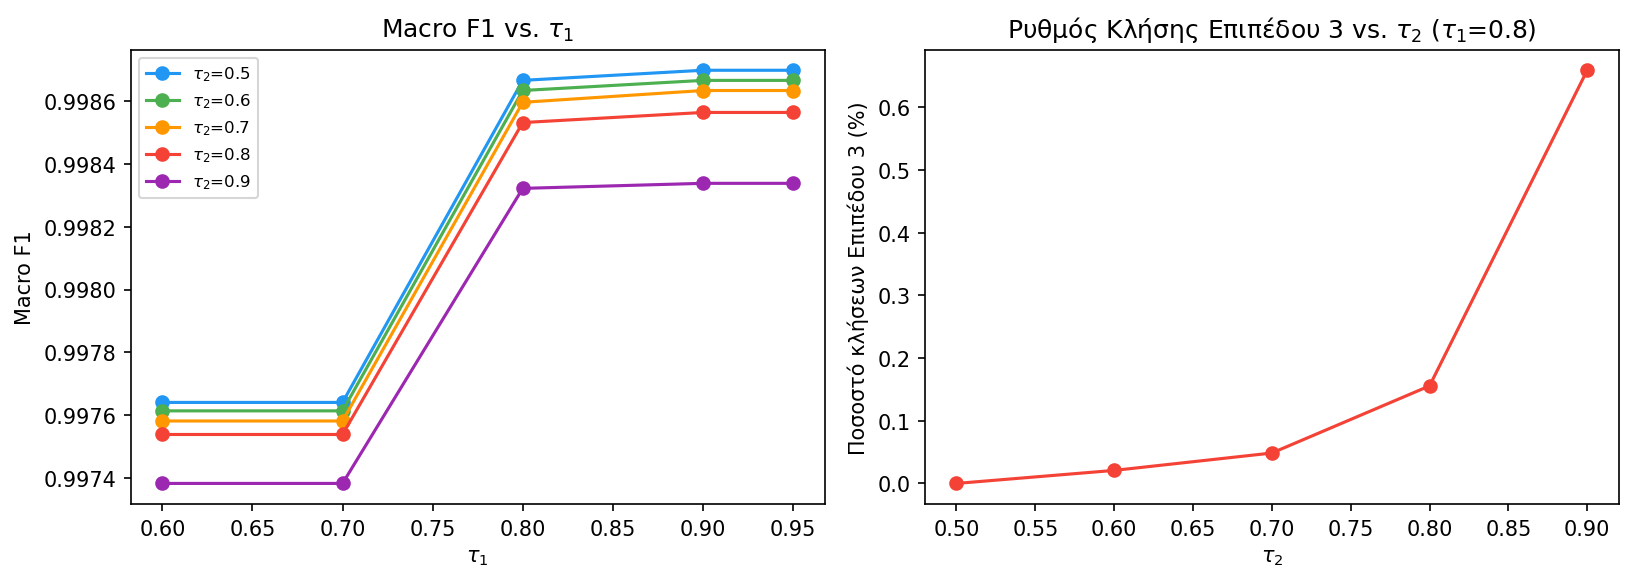
\includegraphics[width=\textwidth]{threshold_ablation}
  \caption{Επέκταση της ανάλυσης ευαισθησίας των ορίων δρομολόγησης. Αριστερά: \en{Macro F1} συναρτήσει του
  $\tau_1$ για το ρεαλιστικό εύρος $\tau_2 \leq 0{,}9$ (\S\ref{sec:ablation}). Κέντρο:
  ποσοστό κλήσεων του Επιπέδου~3 συναρτήσει του $\tau_2$ στο πλήρες επεκταμένο πλέγμα
  ($\tau_1 = \TauOneDefault$), όπου φαίνεται καθαρά το πλατό κοντά στο $\tau_2 = 1$.
  Δεξιά: \en{Macro F1} του υποσυνόλου του Επιπέδου~3 και συνολικό \en{Macro F1} της
  αλυσίδας συναρτήσει του ποσοστού κλήσεων του Επιπέδου~3, στο ίδιο επεκταμένο πλέγμα ---
  η αντίθετη πορεία των δύο καμπυλών αποτυπώνει το εύρημα της παρούσας ενότητας.}
  \label{fig:threshold-ablation-extended}
\end{figure}


\section{Ανάλυση Ζευγών Μηδενικού \en{CN}}
\label{sec:cold-start-results}

Χρησιμοποιώντας τη \texttt{\en{zero\_common\_neighbors\_mask}}
(μηδενικοί κοινοί γείτονες μεταξύ $u$ και $v$) στο σύνολο επικύρωσης, βρίσκουμε
ότι το \ColdStartPct\% των ζευγών (\ColdStartCount{} από \ValSplitSize{},
εξαιρουμένων των αυτοβρόχων) ανήκει στο υποσύνολο μηδενικού \en{CN}.
Μόλις \ColdStartNonCount{} ζεύγη επικύρωσης έχουν έστω έναν κοινό γείτονα, και τα 7 ανήκουν στην
κατηγορία υψηλού \en{CN} και επιλύονται σωστά στο Επίπεδο~1.
Στην πράξη, η
απόδοση ανά επίπεδο στο υποσύνολο μηδενικού \en{CN} ταυτίζεται αριθμητικά με
την συνολική απόδοση ανά επίπεδο του πίνακα~\ref{tab:cascade-tier-results}: το
Επίπεδο~1 χειρίζεται το \TierOnePct\% αυτού του υποσυνόλου με ακρίβεια \TierOneAcc{} και
\en{Macro F1} \TierOneFone{}, το Επίπεδο~2 το \TierTwoPct\% με ακρίβεια \TierTwoAcc{}, και το
Επίπεδο~3 το \TierThreePct\% με ακρίβεια μόλις \TierThreeAcc{}.

Το εύρημα χαρακτηρίζει κυρίως την ακραία αραιότητα του γραφήματος \en{DSAA}: με
μέσο βαθμό \GraphMeanDegree{} (\S\ref{sec:separability-results}), η ύπαρξη κοινού
γείτονα είναι η εξαίρεση.
Δεν αποτελεί μέτρηση του λειτουργικού \en{cold-start}
του \en{CascadeLP}.
Η δρομολόγηση παρακάμπτει το Επίπεδο~1 μόνο όταν τουλάχιστον
ένα άκρο απουσιάζει από το γράφημα, κατάσταση που αναγνωρίζεται από μηδενικές
τιμές και στα τέσσερα δομικά χαρακτηριστικά.
Ένα ζεύγος με μηδενικό \en{CN}
μπορεί να έχει δύο γνωστά άκρα και μη μηδενικό \en{Preferential Attachment},
οπότε εξακολουθεί να αξιολογείται από το Επίπεδο~1.


\section{Ανάλυση του \en{Hard Residual}}
\label{sec:hard-residual}

\subsection{Παραδείγματα Επίλυσης ανά Επίπεδο}
\label{subsec:tier-examples}

Τα συγκεντρωτικά ποσοστά ακρίβειας ανά επίπεδο (\S\ref{sec:cascade-results}) δεν
εξηγούν \textit{γιατί} ένα συγκεκριμένο ζεύγος επιλύεται σε ένα δεδομένο επίπεδο,
ούτε πώς μοιάζει μια λανθασμένη πρόβλεψη σε πραγματικά δεδομένα.
Η ενότητα αυτή παραθέτει ζεύγη πραγματικά αντλημένα από το
\texttt{\en{cascade\_val\_tiers.csv}} (\S\ref{subsec:implementation-architecture}), ένα ανά
συνδυασμό επιπέδου/δυσκολίας/ορθότητας πρόβλεψης, με σκοπό να δείξει ποια πλευρά
των δεδομένων κάθε ταξινομητής βλέπει και πού αποτυγχάνει.
Ο πλήρης κατάλογος
των ζευγών, μαζί με τα ωμά χαρακτηριστικά τους, βρίσκεται στον
Πίνακα~\ref{tab:worked-examples} του Παραρτήματος~\ref{ch:a}.

\subsubsection{Επίπεδο 0 --- Αυτοβρόχοι}

Το Επίπεδο~0 δεν εξετάζει κανένα χαρακτηριστικό· αποφασίζει αποκλειστικά από την
ισότητα $u = v$.
Το ζεύγος \en{(626449, 626449)}, δηλαδή το άρθρο \en{«Young Lake»}
(λίμνη στο πάρκο \en{Adirondack}, Νέα Υόρκη) με τον εαυτό του, έχει ετικέτα θετική
και επιλύεται από τη σύμβαση του Επιπέδου~0, η οποία θεωρεί κάθε αυτοβρόχο θετικό.
Στο σύνολο
εκπαίδευσης όμως υπάρχει ένα μοναδικό αντιπαράδειγμα: το ζεύγος
\en{(74604, 74604)}, το άρθρο \en{«Hartbeespoort Aerial Cableway»}, φέρει ετικέτα
\textit{αρνητική} (\SelfLoopsTrainNeg{} στα \SelfLoopsTrain{} συνολικά, βλ.
\S\ref{sec:leakage-results})\footnote{Δεν έχει βρεθεί εξήγηση γιατί αυτή η
συγκεκριμένη γραμμή φέρει διαφορετική ετικέτα από τις υπόλοιπες 10.220 --- η πιο
πιθανή υπόθεση είναι σφάλμα επισήμανσης κατά την κατασκευή του συνόλου δεδομένων.}.
Ο κανόνας του Επιπέδου~0 προβλέπει θετικά και για τα δύο, άρα αυτή η μία γραμμή
είναι η μοναδική πρόβλεψη σε ολόκληρο το \en{CascadeLP} που είναι λανθασμένη \textit{εκ
κατασκευής} --- όχι λόγω αδυναμίας κάποιου ταξινομητή, αλλά επειδή ο κανόνας
«αυτοσύνδεσμος $\Rightarrow$ θετικό» δεν αφήνει περιθώριο εξαίρεσης για μία ασυνεπή
ετικέτα.

\subsubsection{Επίπεδο 1 --- Δομικοί Ευρετικοί Δείκτες}

\begin{itemize}
  \item \textbf{Ορθή, τετριμμένη λόγω κοινών γειτόνων.} Το γένος εντόμων
  \en{«Molanna»} και το είδος \en{«Molanna ulmerina»} μοιράζονται πολλούς κοινούς
  γείτονες μέσω της κοινής ταξινομικής ιεραρχίας (πρότυπα \en{taxobox}/\en{speciesbox}
  παραπέμπουν και τα δύο σε γένος, οικογένεια, τάξη)· ο αριθμός κοινών γειτόνων
  υπερβαίνει εύκολα το όριο τετριμμένου, το Επίπεδο~1 απαντά ορθά με υψηλή
  αξιοπιστία.
  \item \textbf{Ορθή, υψηλής ομοιότητας κειμένου.} Τα άρθρα \en{«The Golden Mile»}
  (παράκτια περιοχή ερασιτεχνικού ψαρέματος) και \en{«Angling»} (η μέθοδος αλιείας
  καθαυτή) μοιράζονται λεξιλόγιο γύρω από την αλιεία· ο χαρακτηρισμός δυσκολίας
  τα τοποθετεί σε \en{trivial\_high\_textsim}, αλλά και η δομική επικάλυψη αρκεί ώστε
  το Επίπεδο~1 να τα επιλύσει σωστά χωρίς να χρειαστεί κείμενο.
  \item \textbf{Ψευδώς θετικό λόγω προτύπου αποσαφήνισης.} Τα άρθρα \en{«Leaf
  River»} και \en{«Wapello»} είναι και τα δύο σελίδες αποσαφήνισης («may refer
  to:») χωρίς καμία πραγματική σχέση μεταξύ τους.
  Ο χαρακτηρισμός δυσκολίας τα
  βλέπει ως υψηλής ομοιότητας κειμένου (κοινό πρότυπο αποσαφήνισης), αλλά αυτό
  που πραγματικά παραπλανά το Επίπεδο~1 είναι δομικό: σελίδες αποσαφήνισης
  συνδέονται με δεκάδες άσχετους μεταξύ τους κόμβους, πράγμα που τους δίνει
  τεχνητά μεγάλο αριθμό κοινών γειτόνων με \textit{οποιαδήποτε} άλλη σελίδα
  αποσαφήνισης.
  Η πραγματική ετικέτα είναι αρνητική, η πρόβλεψη θετική.
  \item \textbf{Ορθή παρά τον χαρακτηρισμό «δύσκολο».} Η αθλήτρια ενόργανης
  ακροβατικής γυμναστικής \en{«Viktoriya Mikhnovich»} και η χώρα \en{«Belarus»}
  έχουν χαμηλή ομοιότητα κειμένου (βιογραφικό έναντι άρθρου χώρας), οπότε ο
  χαρακτηρισμός δυσκολίας τα βαθμολογεί ως «δύσκολα»· η γειτονιά του γραφήματος όμως
  --- η αθλήτρια συνδέεται με σελίδες της εθνικής ομοσπονδίας και της
  ολυμπιακής αποστολής που με τη σειρά τους συνδέονται με τη χώρα --- δίνει
  επαρκές δομικό σήμα, και το Επίπεδο~1 απαντά σωστά.
  \item \textbf{Ψευδώς θετικό χωρίς προφανή θεματική αιτία.} Το αμφίβιο
  \en{«Plethodontohyla notosticta»} και η φοιτητική αδελφότητα \en{«The Phi Beta
  Kappa Society»} δεν έχουν καμία θεματική σχέση, και η πραγματική ετικέτα είναι
  αρνητική.
  Το Επίπεδο~1 προβλέπει θετικά --- ενδεχομένως λόγω κοινών κόμβων-
  «κόμβων-γέφυρας» (\en{hubs}) στο γράφημα, όπως γενικές κατηγορίες ή έτη ίδρυσης,
  που συνδέουν έμμεσα ζεύγη χωρίς πραγματική σημασιολογική εγγύτητα.
\end{itemize}

\subsubsection{Επίπεδο 2 --- Χαρακτηριστικά Μερών του Λόγου}

\begin{itemize}
  \item \textbf{Ορθή, πρόσωπο--τίτλος.} Ο \en{«Nigel George Paulet, 18th Marquess
  of Winchester»} και ο τίτλος ευγενείας \en{«Marquessate of Winchester»}
  μοιράζονται πυκνή ορολογία γύρω από τη λέξη \en{«Winchester»}/\en{«marquess»}· η
  κατανομή μερών του λόγου (πυκνότητα κύριων ονομάτων, τίτλων) αρκεί για ορθή
  πρόβλεψη.
  \item \textbf{Ψευδώς αρνητικό, αποσαφήνιση προς γεωγραφικό άρθρο.} Η σελίδα
  αποσαφήνισης \en{«Hood River»} θα έπρεπε να συνδέεται με το ομώνυμο γεωγραφικό
  άρθρο (ποταμός στον Καναδά), αλλά η πρόβλεψη είναι αρνητική.
  Η κατανομή μερών
  του λόγου μιας λίστας αποσαφήνισης (κυρίως κύρια ονόματα, ελάχιστα ρήματα)
  διαφέρει αρκετά από αυτήν ενός άρθρου ποταμού ώστε ο ταξινομητής να μην
  αναγνωρίσει τη σχέση αναφοράς --- ένδειξη ότι το επιφανειακό γλωσσολογικό
  σήμα δεν αρκεί εκεί που χρειάζεται η σημασιολογική σχέση «αυτή η σελίδα
  παραπέμπει σε εκείνη».
  \item \textbf{Ορθή, γεωγραφική εγγύτητα.} Το χωριό \en{«No.\ 3 Komarapalayam»}
  (Ταμίλ Ναντού) και ο σιδηροδρομικός σταθμός \en{«Mallur»} χαρακτηρίζονται
  «δύσκολα» λόγω περιορισμένου δομικού σήματος, αλλά μοιράζονται πρότυπα
  υποδομής (\en{infobox settlement}/\en{infobox station}) με παρόμοια κατανομή
  τοπωνυμικών ουσιαστικών, αρκετή ώστε ο \en{PosClassifier} να επιλύσει σωστά τη
  γεωγραφική εγγύτητα.
  \item \textbf{Ψευδώς αρνητικό, ιδίωμα προς ομώνυμο έργο.} Ο αγγλικός
  ιδιωματισμός \en{«Dutch Uncle»} και το ομώνυμο θεατρικό έργο του \en{Simon
  Gray} συνδέονται πραγματικά (το έργο παίρνει τον τίτλο του από τον
  ιδιωματισμό), αλλά η πρόβλεψη είναι αρνητική· η σχέση όρου-προς-έργο-τέχνης
  δεν αποτυπώνεται σε συχνότητες μερών του λόγου, όσο κι αν και οι δύο σελίδες
  μοιράζονται την ίδια φράση-τίτλο.
\end{itemize}

Και στα δύο πρώτα επίπεδα, το επαναλαμβανόμενο μοτίβο είναι ίδιο με αυτό που
περιγράφεται παρακάτω για το Επίπεδο~3: σελίδες αποσαφήνισης και πρότυπα
μορφοποίησης παράγουν ψευδώς θετικά, ενώ σχέσεις αναφοράς/ιδιώματος που
απαιτούν να «διαβαστεί» το νόημα και όχι μόνο η μορφή παράγουν ψευδώς αρνητικά.
Η διαφορά είναι το επίπεδο αφαίρεσης: το Επίπεδο~1 βλέπει μόνο τοπολογία, το
Επίπεδο~2 μόνο κατανομές μερών του λόγου, και κανένα από τα δύο δεν «διαβάζει»
το κείμενο --- αυτό αφήνεται για το Επίπεδο~3.

\subsection[Το Δύσκολο Υπόλοιπο του Επιπέδου 3]{Το Δύσκολο Υπόλοιπο του Επιπέδου~3}
\label{subsec:tier3-hard-residual}

Το υπόλειμμα ζευγών που φτάνει στο Επίπεδο~3 του \en{CascadeLP} \textit{και}
χαρακτηρίζεται «δύσκολο» από τον χαρακτηρισμό διαχωρισιμότητας
(\S\ref{sec:forensics-protocol}) αντιπροσωπεύει το υποσύνολο ζευγών για το οποίο
οι φθηνότερες οικογένειες χαρακτηριστικών γνησίως αποτυγχάνουν: \HardResCount{} ζεύγη στο σύνολο
επικύρωσης (\S\ref{sec:cascade-results}), με ακρίβεια μόλις \HardResAcc{}.

Πριν από την ποιοτική εξέταση, αξίζει να αποκλειστεί μια μη-σημασιολογική εξήγηση: \HardResMissingN{}
από τα \HardResCount{} ζεύγη (\HardResMissingPct\%) περιλαμβάνουν έναν κόμβο με πλήρως ελλιπές κείμενο άρθρου
(τιμή \en{NaN} στο \texttt{\en{nodes.tsv}}), οπότε η ενσωμάτωση \en{sentence-transformer}
δεν διαθέτει ουσιαστικό σήμα εισόδου.
Ένας μόνο κόμβος (\texttt{\en{id=\HardResNodeId{}}}, χωρίς
κείμενο) συμμετέχει σε \HardResNodePairs{} από αυτά τα ζεύγη· σε όλα τα \HardResNodePairs{} η πραγματική ετικέτα είναι
αρνητική, αλλά ο ταξινομητής προβλέπει θετική ετικέτα στο \HardResNodePredPosPct\% από αυτά ---
ουσιαστικά τυχαία πρόβλεψη λόγω απουσίας δεδομένων, όχι αδυναμία σημασιολογικής
συλλογιστικής.
Ωστόσο, η ελλιπής κάλυψη κειμένου \textit{δεν} είναι η κύρια αιτία της
συνολικής κατάρρευσης του Επιπέδου~3: η ακρίβεια στα \HardResCompleteN{} ζεύγη με πλήρες κείμενο και
στις δύο πλευρές είναι \HardResCompleteAcc{}, χειρότερη από την ακρίβεια \HardResIncompleteAcc{} στα \HardResMissingN{} ζεύγη με
ελλιπές κείμενο.
Το γνησίως δύσκολο υποσύνολο είναι εκείνο όπου \textit{υπάρχει}
πλούσιο κείμενο και ο ταξινομητής εξακολουθεί να αποτυγχάνει.

Η χειρωνακτική εξέταση δείγματος από αυτά τα 41 ζεύγη πλήρους κειμένου αναδεικνύει
τρία επαναλαμβανόμενα μοτίβα αποτυχίας:

\begin{itemize}
  \item \textbf{Ομώνυμα σε άσχετους τομείς.} Το άρθρο \en{«FASTRAC 1»} περιγράφει
  διαστημικό δορυφόρο, ενώ το \en{«JCB Fastrac»} περιγράφει γεωργικό ελκυστήρα· τα δύο
  κείμενα μοιράζονται τη λέξη \en{«Fastrac»} αλλά ανήκουν σε εντελώς διαφορετικά
  θεματικά πεδία.
  Η πραγματική ετικέτα είναι θετική (πιθανότατα σύνδεσμος
  αποσαφήνισης λόγω κοινού ονόματος), αλλά η πρόβλεψη είναι αρνητική: η ομοιότητα
  ενσωματώσεων σωστά εντοπίζει τη θεματική απόσταση, λάθος όμως ως προς το αν
  υπάρχει ακμή.
  \item \textbf{Ψευδώς θετικά από κοινό πρότυπο \en{infobox}.} Δύο άρθρα ειδών
  σκαθαριού του γένους \en{Abacetus} (\en{«Abacetus laevigatus»} και ένα δεύτερο
  είδος) μοιράζονται πυκνή ταξινομική ορολογία και πανομοιότυπη δομή προτύπου
  \en{taxobox}, χωρίς καμία πραγματική ακμή μεταξύ τους.
  Η επιφανειακή ομοιότητα
  κειμένου, προερχόμενη από κοινό μορφότυπο και όχι από κοινό περιεχόμενο, οδηγεί σε
  ψευδώς θετική πρόβλεψη.
  \item \textbf{Χαλαρή θεματική συνάφεια.} Το άρθρο αποσαφήνισης \en{«poor me»}
  (τίτλοι τραγουδιών) συνδέεται πραγματικά με το \en{«victim mentality»} (ψυχολογική
  έννοια), μια σχέση νοήματος-προς-τίτλο που απαιτεί βαθύτερη συλλογιστική από την
  ομοιότητα ενσωματώσεων παραγράφου· η πρόβλεψη είναι αρνητική.
\end{itemize}

Στις δύο πρώτες περιπτώσεις η κατεύθυνση του σφάλματος είναι αντίθετη (ψευδώς αρνητικό
έναντι ψευδώς θετικού), αλλά η υποκείμενη αιτία είναι κοινή: η ομοιότητα κειμένου σε
επίπεδο ενσωμάτωσης δεν ταυτίζεται με την ύπαρξη ακμής σε αυτό το σύνολο δεδομένων.
Δύο άρθρα με κοινό όνομα αλλά διαφορετικό αντικείμενο μπορεί να συνδέονται (σύνδεσμος
αποσαφήνισης), ενώ δύο άρθρα με κοινή μορφοποίηση \en{infobox} αλλά ανεξάρτητο
περιεχόμενο μπορεί να μη συνδέονται καθόλου.
Αυτό συνάδει με την τάση υποπρόβλεψης
θετικής ετικέτας που παρατηρήθηκε στη \S\ref{sec:cascade-results} (\TierThreePredPosPct\%
προβλεπόμενα θετικά έναντι \TierThreeTruePosPct\% πραγματικά θετικά): το Επίπεδο~3 τείνει να
ερμηνεύει τη θεματική απόσταση ως απουσία ακμής, κάτι που είναι σωστό στις
περισσότερες περιπτώσεις αλλά όχι στους συνδέσμους αποσαφήνισης/ομωνυμίας.

Το Επίπεδο~3 δεν αποτυγχάνει πάντα σε τέτοια ζεύγη· αξίζει να δούμε και πού
πετυχαίνει, ώστε τα τρία παραπάνω παραδείγματα να μην αφήνουν την εντύπωση
γενικής αδυναμίας.
Το γένος \en{«Abacetus»} εμφανίζεται ξανά, αυτή τη φορά σε
ζεύγος με το εντελώς άσχετο άρθρο \en{«Tidal downsizing»} (υπόθεση σχηματισμού
πλανητών): η πραγματική ετικέτα είναι αρνητική, και εδώ η ομοιότητα
ενσωματώσεων την εντοπίζει σωστά --- σε αντίθεση με το ζεύγος \en{Abacetus}
παραπάνω, δεν υπάρχει κοινό πρότυπο \en{taxobox} που να προκαλεί σύγχυση.
Ομοίως,
το \en{«Niigata Institute of Technology»} (ιδρύθηκε στην πόλη \en{Kashiwazaki}) και
η σελίδα αποσαφήνισης \en{«Kashiwazaki»} συνδέονται πραγματικά, και το Επίπεδο~3
το προβλέπει σωστά χωρίς να χρειάζεται δομική επιβεβαίωση --- η ενσωμάτωση
συλλαμβάνει τη γεωγραφική αναφορά μέσα στο κείμενο του ιδρύματος.

Δύο επιπλέον λανθασμένες προβλέψεις δείχνουν ένα τέταρτο μοτίβο, διαφορετικό
από τα τρία παραπάνω: σχέσεις έργου-προς-δημιουργό ή προσώπου-προς-θεσμικό
κείμενο.
Το μυθιστόρημα \en{«Stormrider»} του συγγραφέα \en{David Gemmell} δεν
συνδέεται, στην πρόβλεψη του Επιπέδου~3, με την ίδια τη σελίδα \en{«David
Gemmell»} --- ενώ η πραγματική ετικέτα είναι θετική.
Η ενσωμάτωση συλλαμβάνει
θεματική εγγύτητα (και τα δύο κείμενα αφορούν φαντασία/λογοτεχνία), αλλά όχι
την ειδικότερη σχέση συγγραφής.
Παρόμοια, ο δικαστής του Ανωτάτου Δικαστηρίου
των \en{ΗΠΑ} \en{«Stephen Breyer»} και ο νόμος \en{«Individuals with Disabilities
Education Act»} έχουν πραγματική θετική ετικέτα, αλλά η πρόβλεψη είναι
αρνητική: η ομοιότητα ενσωμάτωσης δεν αρκεί για να συνδέσει ένα πρόσωπο με ένα
συγκεκριμένο νομοθέτημα, ακόμα κι όταν η σχέση (ο δικαστής έχει εκδώσει
αποφάσεις σχετικές με τον νόμο) είναι πραγματική.
Και στα δύο, το μοτίβο δεν
είναι επιφανειακή ομοιότητα λέξεων όπως στο \en{Fastrac}, αλλά έλλειψη
αναπαράστασης για σχέσεις \textit{δημιουργού--έργου} και
\textit{προσώπου--θεσμικού-κειμένου}, οι οποίες δεν εκφράζονται ρητά στο σώμα
κειμένου του ενός ή του άλλου άρθρου.


\section{Σύγκριση Αποτελεσματικότητας}
\label{sec:efficiency}

Πέρα από την ακρίβεια, η κεντρική υπόσχεση της αρχιτεκτονικής με επίπεδα είναι
η \textit{οικονομία υπολογισμού}: τα φθηνά επίπεδα πρέπει να απορροφούν τη
συντριπτική πλειονότητα των ζευγών, αφήνοντας το ακριβό σημασιολογικό επίπεδο για
ένα ελάχιστο υπόλειμμα.
Η ενότητα αυτή ποσοτικοποιεί αυτή την υπόσχεση.

\subsection{Ρυθμός Επεξεργασίας}
\label{subsec:throughput}

Στην τελική διαμόρφωση μόνο με ευρετικά χαρακτηριστικά (\S\ref{sec:cascade-routing}),
το \en{CascadeLP} επεξεργάζεται τα \ValSplitSize{} ζεύγη του συνόλου επικύρωσης σε
\ThroughputSec~δευτερόλεπτα σε \en{CPU} (ταχύτερη από τρεις εκτελέσεις), ήτοι περίπου
\ThroughputRate{} ζεύγη ανά δευτερόλεπτο ή \ThroughputLatency~ms ανά ζεύγος.
Η μέτρηση αφορά αποκλειστικά
το κόστος δρομολόγησης και ταξινόμησης πάνω σε ήδη υπολογισμένα χαρακτηριστικά· το
κόστος εξαγωγής των χαρακτηριστικών --- κυρίως η κωδικοποίηση \en{sentence-transformer}
του Επιπέδου~3 --- βρίσκεται εκτός αυτής της μέτρησης και αποτελεί το κυρίαρχο
υπολογιστικό κόστος του pipeline.

Στα προεπιλεγμένα όρια, το 99{,}95\% των ζευγών (Επίπεδα~1 και~2,
\TierOneCount{} + \TierTwoCount{} ζεύγη) λαμβάνει απόφαση πριν από το
σημασιολογικό επίπεδο, και μόλις \TierThreeCount{} ζεύγη (\TierThreePct\%) λαμβάνουν
την τελική πρόβλεψη του Επιπέδου~3.
Οι αριθμοί αυτοί μετρούν δρομολόγηση πάνω σε
ήδη υπολογισμένα χαρακτηριστικά.
Υποδεικνύουν πιθανή εξοικονόμηση σε μια μελλοντική
υλοποίηση κατ' απαίτηση, αλλά δεν αποτελούν μέτρηση των κωδικοποιήσεων που
αποφεύχθηκαν στο παρόν πείραμα.

\subsection[Ποσοστό Δρομολόγησης στο Επίπεδο 3 ανά Όριο]{Ποσοστό Δρομολόγησης στο Επίπεδο~3 ανά Όριο}
\label{subsec:tier3-rate}

Το ποσοστό δρομολόγησης στο Επίπεδο~3 (σημασιολογικό επίπεδο βασισμένο σε
\en{sentence-transformer}) καθορίζεται σχεδόν αποκλειστικά από το όριο $\tau_2$: το
$\tau_1$ ρυθμίζει τον καταμερισμό μεταξύ Επιπέδων~1 και~2 και έχει αμελητέα επίδραση
στο υπόλειμμα που κλιμακώνεται πέρα από το Επίπεδο~2.
Ο πίνακας~\ref{tab:tier3-rate} δείχνει το ποσοστό αυτό ως συνάρτηση του $\tau_2$ για $\tau_1 = 0{,}8$ (προεπιλογή).

\begin{table}[htbp]
  \centering
  \begin{tabular}{lrrrrr}
    \toprule
    $\tau_2$ & 0{,}5 & 0{,}6 & 0{,}7 & 0{,}8 & 0{,}9 \\
    \midrule
    Ποσοστό δρομολόγησης στο Επίπεδο~3 & \AblTThreeRateZeroFive\% & \AblTThreeRateZeroSix\% & \AblTThreeRateZeroSeven\% & \AblTThreeRateZeroEight\% & \AblTThreeRateZeroNine\% \\
    \bottomrule
  \end{tabular}
  \caption{Ποσοστό δρομολόγησης στο Επίπεδο~3 ως συνάρτηση του ορίου $\tau_2$
  ($\tau_1 = \TauOneDefault$, σύνολο επικύρωσης n=\ValSplitSize{}).}
  \label{tab:tier3-rate}
\end{table}

Ακόμη και στο πιο επιτρεπτικό σημείο ολόκληρου του πλέγματος ($\tau_1 = 0{,}95$,
$\tau_2 = 0{,}9$), το Επίπεδο~3 χειρίζεται μόλις το \TierThreeCallRateMax\% των ζευγών· στα
προεπιλεγμένα όρια ($\tau_1 = \TauOneDefault$, $\tau_2 = \TauTwoDefault$) το ποσοστό πέφτει στο
\AblTThreeRateZeroSeven\% (\TierThreeCount{} ζεύγη).
Αυτά τα νούμερα αφορούν το ρεαλιστικό εύρος λειτουργίας ($\tau_2 \leq 0{,}9$)· η
\S\ref{subsec:force-tier3} εξετάζει ξεχωριστά τι συμβαίνει αν το $\tau_2$ σφίξει πολύ
πέρα από αυτό, και δείχνει ότι το ποσοστό δρομολόγησης μπορεί μεν να εξαναγκαστεί πολύ
υψηλότερα, αλλά χωρίς κανένα όφελος ακρίβειας.
Το ακριβό σημασιολογικό επίπεδο λειτουργεί, επομένως, ως
σπάνια ενεργοποιούμενη δικλείδα ασφαλείας και όχι ως βασικός φορέας εργασίας ---
συμπέρασμα που ενισχύει την επιλογή να μη γίνεται χαλάρωση του $\tau_2$ πέρα από την
προεπιλογή, δεδομένης της αναξιοπιστίας του επιπέδου στο υπόλειμμα που φτάνει ως εκεί
(\S\ref{sec:hard-residual}).


\section{Ανάλυση Σφαλμάτων}
\label{sec:error-analysis}

Το \en{CascadeLP} κάνει \CascadeTotalErrors{} σφάλματα ταξινόμησης στις \ValSplitSize{} ζεύγη επικύρωσης.
Από
αυτά, το \CascadeErrorsHardPct\% (\CascadeErrorsHardN{} σφάλματα) προέρχεται από ζεύγη που χαρακτηρίζονται \en{hard}
από το πρωτόκολλο χαρακτηρισμού δυσκολίας (\S\ref{sec:forensics-protocol}), και το
\CascadeErrorsTrivialPct\% (\CascadeErrorsTrivialN{} σφάλματα) από τετριμμένα ζεύγη υψηλής ομοιότητας κειμένου --- κανένα
σφάλμα δεν προέρχεται από αυτοβρόχους ή ζεύγη υψηλού \en{CN}, όπου το Επίπεδο~0 και το
Επίπεδο~1 αντίστοιχα είναι αλάνθαστα.

Το μοντέλο αναφοράς \en{TF-IDF + SVM} (\S\ref{sec:svm-baseline}), εκπαιδευμένο και
αξιολογημένο στην ίδια διαίρεση επικύρωσης, κάνει \SvmTotalErrors{} σφάλματα --- περίπου
\CascadeVsSvmRatio{} φορές περισσότερα.
Το προφίλ σφαλμάτων του συγκεντρώνεται στην κατηγορία \en{hard}
σχεδόν στον ίδιο βαθμό με το \en{CascadeLP}: \SvmErrorsHardPct\% από ζεύγη \en{hard} και \SvmErrorsTrivialPct\%
από τετριμμένα ζεύγη υψηλής ομοιότητας κειμένου.
Ο πίνακας~\ref{tab:error-comparison}
συνοψίζει τη σύγκριση.

\begin{table}[htbp]
  \centering
  \begin{tabular}{lrrrr}
    \toprule
    & \multicolumn{2}{c}{\textbf{\en{CascadeLP}}} & \multicolumn{2}{c}{\textbf{\en{SVM}}} \\
    \textbf{Κατηγορία Δυσκολίας} & \textbf{Σφάλματα} & \textbf{\%} & \textbf{Σφάλματα} & \textbf{\%} \\
    \midrule
    \en{hard}                  & \CascadeErrorsHardN{} & \CascadeErrorsHardPct\% & \SvmErrorsHardN{} & \SvmErrorsHardPct\% \\
    Υψηλή Ομοιότητα Κειμένου   & \CascadeErrorsTrivialN{}  & \CascadeErrorsTrivialPct\%  & \SvmErrorsTrivialN{}  & \SvmErrorsTrivialPct\%  \\
    \midrule
    \textbf{Σύνολο}             & \textbf{\CascadeTotalErrors{}} & \textbf{100\%} & \textbf{\SvmTotalErrors{}} & \textbf{100\%} \\
    \bottomrule
  \end{tabular}
  \caption{Σύγκριση προφίλ σφαλμάτων \en{CascadeLP} έναντι \en{SVM} ανά κατηγορία
  δυσκολίας, σύνολο επικύρωσης (n=\ValSplitSize{}).}
  \label{tab:error-comparison}
\end{table}

Το \en{SVM} υποαποδίδει ακόμη και στην κατηγορία «τετριμμένη» υψηλής ομοιότητας
κειμένου: ακρίβεια \SvmHighTextsimAcc{} αλλά \en{Macro F1} μόλις \SvmHighTextsimFone{} σε αυτό το υποσύνολο ---
το ίδιο μοτίβο κατάρρευσης λόγω ανισορροπίας κλάσεων που παρατηρήθηκε στο Επίπεδο~1
του \en{CascadeLP} (\S\ref{sec:cascade-results}).
Στην κατηγορία \en{hard}, το \en{SVM}
πετυχαίνει ακρίβεια \SvmHardAcc{} και \en{Macro F1} \SvmHardFone{}, ενώ το \en{CascadeLP}
πετυχαίνει \CascadeHardAcc{} και \CascadeHardFone{} αντίστοιχα στο ίδιο υποσύνολο --- μια διαφορά που δεν
αποδίδεται σε κοινή χρήση της ομοιότητας \en{TF-IDF}: αυτή αποτελεί τη μοναδική
είσοδο του \en{SVM}, ενώ δεν χρησιμοποιείται από τους ταξινομητές του
\en{CascadeLP}.
Η διαφορά συνδέεται με τον σημαντικά μεγαλύτερο όγκο δεδομένων
εκπαίδευσης που αξιοποιεί το \en{CascadeLP} και με τον συνδυασμό των δομικών
χαρακτηριστικών του Επιπέδου~1, των χαρακτηριστικών \en{POS} του Επιπέδου~2 και
της ομοιότητας \en{Sentence-Transformer} του Επιπέδου~3.
Το Επίπεδο~2 απορροφά το \TierTwoPct\%
των ζευγών επικύρωσης με σχεδόν μηδενικό ποσοστό σφάλματος.
Και τα δύο μοντέλα
συγκεντρώνουν τη μεγάλη πλειονότητα των σφαλμάτων τους στην κατηγορία \en{hard}, σε
σχεδόν πανομοιότυπη αναλογία (\CascadeErrorsHardPct\% έναντι \SvmErrorsHardPct\%) παρά τη 64-πλάσια διαφορά
στο απόλυτο πλήθος σφαλμάτων --- εύρημα που επιβεβαιώνει τη συνέπεια του πρωτοκόλλου
χαρακτηρισμού δυσκολίας ως προγνωστικού δείκτη πραγματικής δυσκολίας ταξινόμησης,
ανεξάρτητα από την οικογένεια μοντέλου.
Ανάλυση ανά σύνολο δεδομένων εκτελείται στην \S\ref{sec:wiki-fresh}, όπου το
\en{CascadeLP} αξιολογείται σε ένα δεύτερο, ανεξάρτητα κατασκευασμένο σύνολο
δεδομένων.




\section{Συγκριτική Ερμηνεία των Δύο Συνόλων}
\label{sec:cross-dataset-discussion}

Τα αποτελέσματα του Πίνακα~\ref{tab:wiki-fresh-results} αλλάζουν την ερμηνεία
της αρχιτεκτονικής χωρίς να αναιρούν τον έλεγχο του \en{DSAA 2023}.
Στο
\en{DSAA}, ένας μικρός αριθμός τιμών του πρώτου άκρου καθορίζει σχεδόν πλήρως
την ετικέτα και ο κανόνας αναζήτησης αναπαράγει τη σχεδόν τέλεια επίδοση.
Το αυτόνομο μοντέλο αναφοράς \en{POS} (0{,}9988) υπερβαίνει μάλιστα οριακά το
\en{CascadeLP} (0{,}9986), άρα η αλυσίδα δεν αποτελεί την καλύτερη μέθοδο στο
αρχικό σύνολο επικύρωσης.
Στο
ανεξάρτητο σύνολο, τα αρνητικά ζεύγη δειγματοληπτούνται από τον ίδιο πληθυσμό
κόμβων και δεν συγκεντρώνονται σε ένα μικρό σύνολο πηγών.
Η επίδοση πέφτει σε
ρεαλιστικότερο επίπεδο, ενώ η σχετική κατάταξη των οικογενειών χαρακτηριστικών
μεταβάλλεται ουσιωδώς.

Η σημαντικότερη διαφορά αφορά τη δομή.
Στο \en{DSAA 2023}, το γράφημα έχει
μέσο βαθμό \GraphMeanDegree{} και τα χαρακτηριστικά γειτονιάς παρέχουν ελάχιστο
σήμα στα περισσότερα ζεύγη.
Στο δεύτερο σύνολο, το γράφημα εκπαίδευσης έχει
μέσο βαθμό \WfMeanDegree{} και ο αυτόνομος δομικός ταξινομητής πετυχαίνει
\en{Macro F1} = \WfStructuralFone{}.
Το \en{CascadeLP} βελτιώνει αυτή την τιμή
σε \WfCascadeFone{} συνδυάζοντας τα δομικά και κειμενικά επίπεδα, ενώ
δρομολογεί το \WfTierOnePct\% των ζευγών στο Επίπεδο~1.
Το εύρημα υποστηρίζει
ότι η αρχιτεκτονική μπορεί να εκμεταλλευτεί πραγματικό δομικό σήμα όταν αυτό
είναι διαθέσιμο.

Η σύγκριση δεν αποδεικνύει ότι το νέο σύνολο αποτελεί καθολικά δυσκολότερο ή
πλήρως αντιπροσωπευτικό πεδίο αξιολόγησης.
Η διάσχιση \en{BFS} (με αφετηρία το
άρθρο \en{«Computer science»}) δημιουργεί ένα
θεματικά και τοπολογικά συνεκτικό υπογράφημα, ενώ τα ομοιόμορφα τυχαία αρνητικά
είναι πιθανό να είναι ευκολότερα από αρνητικά που ταιριάζονται ως προς βαθμό,
θέμα ή κειμενική ομοιότητα.
Επιπλέον, \WfTextEmptyN{} κόμβοι δεν διαθέτουν
κείμενο.
Το διαγνωστικό υποσύνολο των \WfMissingTextCount{} ζευγών επικύρωσης με
τουλάχιστον ένα τέτοιο άκρο δίνει \en{Macro F1} = \WfMissingTextFone{}, αλλά δεν
απομονώνει αιτιακά την επίδραση της απουσίας κειμένου, επειδή τα ίδια ζεύγη μπορεί
να διαθέτουν ισχυρό δομικό σήμα.
Το νέο
πείραμα παρέχει συνεπώς ισχυρότερη ένδειξη για το \en{CascadeLP} από το
\en{DSAA 2023}, αλλά όχι τελική απόδειξη γενίκευσης σε κάθε γράφημα με
κειμενικά χαρακτηριστικά.

Τέλος, τα προηγούμενα αποτελέσματα του διαγωνισμού \en{DSAA 2023} παραμένουν
έγκυρα ως βαθμολογίες στο συγκεκριμένο \en{leaderboard}.
Επειδή όμως οι
δημοσιευμένες μελέτες δεν ελέγχουν τον κανόνα του πρώτου άκρου, οι σχεδόν
τέλειες βαθμολογίες τους δεν αρκούν για να τεκμηριώσουν ότι τα αντίστοιχα
μοντέλα έμαθαν τη σχέση μεταξύ των δύο άρθρων.
Το συμπέρασμα αφορά την
αποδεικτική ισχύ του συνόλου αξιολόγησης και όχι την ορθότητα της υλοποίησης
των προηγούμενων λύσεων.
                % Ch.5 Ανάλυση               \ref{chap:analysis}
    % Chapter 6: Conclusion — summary of contributions, limitations, future work
\selectlanguage{greek}

\chapter{Συμπέρασμα}
\label{ch:conclusion}

\section{Σύνοψη Συνεισφορών}
\label{sec:summary}

Η εργασία εισήγαγε το \en{CascadeLP}, μια τετραεπίπεδη αρχιτεκτονική πρόβλεψης
ακμών που δρομολογεί κάθε ζεύγος μέσω προοδευτικά ακριβότερων οικογενειών
χαρακτηριστικών.
Η αρχιτεκτονική αξιολογήθηκε σε δύο σύνολα δεδομένων με
διαφορετική κατασκευή.
Η διπλή αυτή αξιολόγηση αποδείχθηκε ουσιώδης: το πρώτο
σύνολο παρείχε σύγκριση με τον διαγωνισμό \en{DSAA 2023}, ενώ το δεύτερο επέτρεψε
να ελεγχθεί η συμπεριφορά του πλαισίου χωρίς τη συγκεκριμένη στρέβλωση στη
δειγματοληψία που εντοπίστηκε στο πρώτο.

Στο \en{DSAA 2023}, το \en{CascadeLP} πέτυχε \en{Macro F1} =
\CascadeValFone{} υπό το αρχικό πρωτόκολλο επικύρωσης και
\KaggleBaselinePublic{} στο δημόσιο \en{leaderboard}.
Οι τιμές αυτές είναι
έγκυρες ως βαθμολογίες στο συγκεκριμένο πεδίο αξιολόγησης, αλλά δεν αποτελούν
από μόνες τους απόδειξη σχεσιακής πρόβλεψης.
Ο έλεγχος επικάλυψης βρήκε μόνο
\LeakageExact{} ακριβή και \LeakageReversed{} αντεστραμμένα ζεύγη σε
\TestPairs{} ζεύγη ελέγχου, όμως ο ευρύτερος έλεγχος ακεραιότητας αποκάλυψε ότι
\HubCount{} από τις
\HubUniqueSourceCount{} μοναδικές τιμές του πρώτου άκρου στο \en{DSAA 2023}
αντιστοιχούν στο \HubRowPct\% των γραμμών εκπαίδευσης και είναι
\HubPurityPct\% αρνητικές, ενώ κάθε άλλη γραμμή είναι θετική.
Ένας απλός
πίνακας αναζήτησης σε αυτές τις \HubCount{} τιμές πετυχαίνει \en{Macro F1} =
\HubLookupFone{}, και οι προβλέψεις του \en{CascadeLP} συμφωνούν μαζί του στο
\HubValAgreementPct\% του συνόλου επικύρωσης.
Το \en{DSAA 2023} δεν μπορεί συνεπώς να διακρίνει την
εκμάθηση σχέσεων από την αναγνώριση ενός μικρού συνόλου πηγών.
Το ίδιο όριο
ισχύει για τις προηγούμενες σχεδόν τέλειες λύσεις του διαγωνισμού: οι
δημοσιευμένες βαθμολογίες τους δεν αποδεικνύουν ποιο από τα δύο φαινόμενα
έμαθαν τα μοντέλα.

Στο δεύτερο σύνολο πραγματικών υπερσυνδέσμων της Απλής Αγγλικής
\en{Wikipedia}, το ίδιο αρχιτεκτονικό σχήμα επανεκπαιδεύτηκε από την αρχή με
ομαδοποιημένη διαίρεση και απόκρυψη της ακμής-στόχου.
Οι δομικοί ευρετικοί
δείκτες πέτυχαν \en{Macro F1} = \WfStructuralFone{}, ενώ το \en{CascadeLP}
πέτυχε \WfCascadeFone{}, υψηλότερα από κάθε μεμονωμένη οικογένεια
χαρακτηριστικών.
Το \WfTierOnePct\% των ζευγών επιλύθηκε στο Επίπεδο~1, το
\WfTierTwoPct\% στο Επίπεδο~2 και το \WfTierThreePct\% έφτασε στο Επίπεδο~3.
Αυτό αποτελεί την ισχυρότερη ένδειξη της εργασίας ότι η αρχιτεκτονική συνδυάζει
χρήσιμα τις οικογένειες χαρακτηριστικών και δρομολογεί τη μεγάλη πλειονότητα
των ζευγών στο φθηνότερο επίπεδο όταν υπάρχει πραγματικό δομικό σήμα.
Στον συμπληρωματικό έλεγχο με αραιό γράφημα, η επίδοση στα δύσκολα αρνητικά
πέφτει σε \WsRandomHardCascadeFone{} όταν η εκπαίδευση χρησιμοποιεί μόνο
τυχαία αρνητικά. Η μικτή εκπαίδευση την αυξάνει σε
\WsMixedHardCascadeFone{}, υψηλότερα από το αυτόνομο
\en{Embedding} (\WsMixedHardEmbeddingFone{}), με κόστος
\WsRandomCost{} μονάδες \en{Macro F1} στο σύνολο τυχαίων αρνητικών.

Τα τρία ερευνητικά ερωτήματα απαντώνται επομένως με διαφορετικό βαθμό
βεβαιότητας.
Πρώτον, στο ανεξάρτητο σύνολο το \en{CascadeLP} υπερβαίνει την
ισχυρότερη αυτόνομη οικογένεια κατά \WfCascadeDeltaStructural{} μονάδες
\en{Macro F1}, με 95\% διάστημα από επαναδειγματοληψία \en{paired bootstrap}
[\WfCascadeDeltaStructuralCiLow{}, \WfCascadeDeltaStructuralCiHigh{}]. Δεύτερον,
η δρομολόγηση επιλύει το \WfTierOnePct\% των ζευγών στο δομικό επίπεδο και μόνο
το \WfTierThreePct\% φτάνει στο τελευταίο, στοιχείο που τεκμηριώνει την επιλεκτική
κλιμάκωση και τη δυνατότητα μελλοντικής εξαγωγής χαρακτηριστικών κατά απαίτηση,
όχι ήδη μετρημένη ισόποση εξοικονόμηση.
Τρίτον, ο έλεγχος του \en{DSAA 2023}
δείχνει ότι οι σχεδόν τέλειες βαθμολογίες του δεν μπορούν να απομονώσουν τη
σχεσιακή μάθηση από τη στρέβλωση στην επιλογή της πηγής των αρνητικών παραδειγμάτων.

Το μοντέλο αναφοράς \en{TF-IDF + SVM} διατηρήθηκε ως κλασική σημασιολογική
σύγκριση.
Η εκπαίδευση \en{SVC} με πυρήνα ακτινικής βάσης κλιμακώνεται
τετραγωνικά έως κυβικά ως προς το πλήθος δειγμάτων, γι' αυτό στο \en{DSAA 2023}
χρησιμοποιήθηκε στρωματοποιημένο υποσύνολο \SvmSampleSize{} ζευγών.
Η σύγκριση
τοποθετεί το \en{CascadeLP} όχι μόνο απέναντι στις επιμέρους οικογένειες
χαρακτηριστικών του, αλλά και απέναντι σε μια καθιερωμένη μέθοδο με δυσμενέστερο
κόστος εκπαίδευσης.

\section{Περιορισμοί}
\label{sec:limitations-cost}

Η εργασία αξιολογεί το \en{CascadeLP} σε δύο σύνολα υπερσυνδέσμων της
\en{Wikipedia}, όχι όμως σε διαφορετικό τύπο \en{TAG}.
Η επανεκπαίδευση στο
δεύτερο σύνολο ελέγχει την αρχιτεκτονική υπό διαφορετική κατασκευή δεδομένων,
όχι μεταφορά μάθησης χωρίς επανεκπαίδευση ούτε γενίκευση σε άλλο πεδίο εφαρμογής.
Επιπλέον, το δεύτερο σύνολο προέρχεται από διάσχιση \en{BFS} με έναν σπόρο.
Το αρχικό του πρωτόκολλο χρησιμοποιεί ομοιόμορφα τυχαία αρνητικά· ο
συμπληρωματικός έλεγχος με αρνητικά δύο βημάτων δείχνει ουσιώδη πτώση της
επίδοσης και μερική ανάκτησή της μετά από μικτή εκπαίδευση.
Το εύρημα καλύπτει συγκεκριμένη κατασκευή δύσκολων ζευγών, όχι κάθε τρόπο
με τον οποίο τα αρνητικά παραδείγματα μπορούν να μεταβάλουν τη δυσκολία.
Η αναφορά βασίζεται σε έναν σπόρο διάσχισης, μία διαίρεση ανά πρωτόκολλο και μία
εκπαίδευση ανά μοντέλο και εκδοχή αρνητικών.
Συνεπώς, δεν ποσοτικοποιεί τη μεταβλητότητα μεταξύ
διαφορετικών σπόρων, διαιρέσεων και επανεκπαιδεύσεων.
Η επαναδειγματοληψία \en{paired bootstrap} των προβλέψεων επικύρωσης και του
δύσκολου συνόλου ελέγχου παρέχει διαστήματα αβεβαιότητας για τις συγκεκριμένες
σταθερές εκτελέσεις, αλλά δεν υποκαθιστά αυτή την πολλαπλή επανεκτέλεση.
Επιπλέον, στο υποσύνολο μηδενικού \en{CN} του δεύτερου συνόλου το \en{Macro F1}
πέφτει σε \WfZeroCnFone{} και η ανάκληση της θετικής κλάσης σε
\WfZeroCnPositiveRecall{}.
Η συνολική υπεροχή του \en{CascadeLP} τεκμηριώνει τον
συνδυασμό των επιπέδων όταν υπάρχει δομικό σήμα, αλλά δεν τεκμηριώνει αξιόπιστη
πρόβλεψη θετικών ακμών όταν αυτό απουσιάζει.
Το λειτουργικό υποσύνολο
\en{cold-start} περιέχει μόνο \WfColdStartCount{} ζεύγη και δεν επαρκεί για
ξεχωριστό ισχυρό συμπέρασμα.

Η μέτρηση αποτελεσματικότητας της παρούσας υλοποίησης αφορά τη δρομολόγηση και
ταξινόμηση πάνω σε ήδη υπολογισμένα χαρακτηριστικά.
Οι ενσωματώσεις
\en{Sentence-Transformer} υπολογίστηκαν πριν από τη δρομολόγηση για όλους τους
διαθέσιμους κόμβους, επομένως το ποσοστό κλήσεων του Επιπέδου~3 δεν ισούται με
ίση ποσοστιαία μείωση του συνολικού κόστους κωδικοποίησης.
Τέτοια εξοικονόμηση
είναι δυνατή σε υλοποίηση με παραγωγή χαρακτηριστικών κατά απαίτηση και κρυφή
μνήμη ανά κόμβο, αλλά δεν μετρήθηκε ενδογενώς στα παρόντα πειράματα.

Το Επίπεδο~3 (\texttt{\en{EmbeddingClassifier}}) παραμένει αναξιόπιστο στο μικρό
υπόλειμμα ζευγών που το φτάνει (\TierThreeAcc{} ακρίβεια σε \TierThreeCount{} ζεύγη).
Τα ζεύγη αυτού του υπολείμματος που δεν διαχωρίζονται από τα απλά κριτήρια ---
ιδίως εκείνα με πλήρες κείμενο και στις δύο πλευρές,
όπου η ακρίβεια είναι ακόμη χαμηλότερη (\HardResCompleteAcc{}) από το υποσύνολο με ελλιπές
κείμενο --- δεν επιλύονται επαρκώς από την ομοιότητα συνημίτονου ενσωματώσεων
\en{sentence-transformer}.
Το αποτέλεσμα δεν αποδεικνύει ποια πρόσθετη μορφή
πληροφορίας απαιτείται για την επίλυσή τους.
Επιπλέον, οι ετικέτες
«τετριμμένου ζεύγους» του χαρακτηρισμού διαχωρισιμότητας προκύπτουν από ένα όριο
εκατοστημορίου ($\alpha = 0{,}01$) στην κατανομή της αρνητικής κλάσης --- μια
σχεδιαστική επιλογή, όχι μια αντικειμενική διαμέριση του συνόλου δεδομένων.
Το πρωτόκολλο μεταφοράς μάθησης εκτός συνόλου δεδομένων
(\S\ref{sec:generalization-protocol})---εκπαίδευση στο ένα σύνολο, αξιολόγηση
χωρίς περαιτέρω εκπαίδευση σε άλλο---δεν εκτελέστηκε.

Η εργασία αντιμετωπίζει σκόπιμα την πρόβλεψη υπερσυνδέσμων ως πρόβλεψη
\textit{μη κατευθυνόμενης συνδεσιμότητας} μετά από συμμετροποίηση, όχι ως
πρόβλεψη της πραγματικής, κατευθυνόμενης σχέσης παραπομπής
(\S\ref{sec:problem-definition})· η επέκταση σε κατευθυνόμενη πρόβλεψη θα
απαιτούσε ανακατασκευή γραφήματος, χαρακτηριστικών και δειγματοληψίας
αρνητικών και παραμένει εκτός εύρους της παρούσας εργασίας.
Στο ίδιο πνεύμα, ο
έλεγχος αντιστροφής άκρων της \S\ref{sec:endpoint-swap} δείχνει ότι ο
\texttt{\en{PosClassifier}} αλλάζει πρόβλεψη στο \SwapLabelChangePct\% των
ζευγών επικύρωσης όταν αντιστρέφεται η σειρά $u, v$ (\SwapNegClassChangePct\%
στα αρχικά αρνητικά έναντι \SwapPosClassChangePct\% στα αρχικά θετικά), λόγω
της μη-συμμετρικής συνένωσης χαρακτηριστικών \en{POS}
(\S\ref{subsec:pos-features}).
Το εύρημα δεν αμφισβητεί τη συμμετρική
διατύπωση του προβλήματος, αλλά αναδεικνύει περιορισμό της συγκεκριμένης
υλοποίησης του Επιπέδου~2, ο οποίος δεν διορθώθηκε στην παρούσα εργασία.
Επιπλέον, ο επαναληπτικός έλεγχος της κατασκευής γραφήματος
(\S\ref{subsec:data-splits}) δείχνει ότι \AuditValPositivesInGraph{} από τα
\AuditValN{} θετικά ζεύγη επικύρωσης του αρχικού πρωτοκόλλου \en{DSAA} έχουν
ήδη συνεισφέρει ακμή στο γράφημα που χρησιμοποιείται για τα δομικά
χαρακτηριστικά· οι σχετικές τιμές \en{Macro F1} χαρακτηρίζονται συνεπώς ως
αξιολόγηση ακμών σε \en{transductive} διαίρεση με κοινούς κόμβους και με
διαρροή των ακμών επικύρωσης στο γράφημα, όχι ως ανεξάρτητη επικύρωση.
Τέλος, η σύγκριση με το \en{SVM} (\S\ref{sec:svm-results})
συμπληρώθηκε με \MatchedNSeeds{} επαναλήψεις ίσου όγκου εκπαίδευσης
(\MatchedSampleSize{} ζεύγη ανά μοντέλο). Το \en{SVM} πέτυχε
\en{Macro F1} = \MatchedTfidfSvmFone{}, έναντι \MatchedCascadeFone{} του
\en{CascadeLP} και \MatchedPosFone{} του αυτόνομου \en{POS}. Η σύγκριση είναι
δίκαιη ως προς τον αριθμό εποπτευόμενων ζευγών και τον προϋπολογισμό
επισημασμένων ζευγών για την κατασκευή του γραφήματος,
αλλά παραμένει εντός του \en{DSAA 2023} και επομένως υπόκειται στη στρέβλωση
στη δειγματοληψία αρνητικών παραδειγμάτων.
Η επανεκπαίδευση από την
αρχή σε ανεξάρτητο σύνολο δεδομένων \en{Wikipedia} (\S\ref{sec:wiki-fresh})
δείχνει ότι η αρχιτεκτονική συμπεριφέρεται όπως σχεδιάστηκε όταν απουσιάζουν τα
ζητήματα ακεραιότητας του \en{DSAA 2023}, αλλά δεν ελέγχει αν αναπαραστάσεις
εκπαιδευμένες στο ένα σύνολο δεδομένων μεταφέρονται σε άλλο χωρίς
επανεκπαίδευση.

\section{Μελλοντική Έρευνα}
\label{sec:future-work}

Η σαφέστερη κατεύθυνση που προκύπτει άμεσα από αυτή την εργασία είναι η
εφαρμογή μιας \textit{inductive} μεθόδου αναπαράστασης κόμβων, όπως το \en{GraphSAGE}, ή γενικότερα με ένα \en{Graph Neural Network (GNN)} που υπολογίζει την αναπαράσταση ενός κόμβου από τα χαρακτηριστικά και τη γειτονιά του.
Ένα τέτοιο \en{GNN} θα μπορούσε, μέσω \en{message passing} πάνω σε χαρακτηριστικά κόμβων (π.χ. \en{TF-IDF} ή \en{sentence-transformer} ενσωματώσεις κειμένου άρθρου), να παραγάγει αναπαράσταση για κόμβο που δεν συμμετείχε σε καμία ακμή εκπαίδευσης και ενδεχομένως να αντικαταστήσει ένα ή περισσότερα επίπεδα της αλυσίδας.

Δεύτερη κατεύθυνση είναι η τυπική μεταφορά μάθησης μεταξύ συνόλων δεδομένων
\en{TAG}---εκπαίδευση στο ένα, αξιολόγηση χωρίς περαιτέρω εκπαίδευση στο
άλλο---που παραμένει ανοιχτή παρά την επανεκπαίδευση από την αρχή σε
ανεξάρτητο σύνολο δεδομένων \en{Wikipedia} της \S\ref{sec:wiki-fresh}, καθώς
και η επέκταση αυτής της επικύρωσης σε συνόλα δεδομένων εκτός \en{Wikipedia}
(π.χ.\ αναφορές επιστημονικών άρθρων, ή γραφήματα κοινωνικών δικτύων με
κειμενικά προφίλ χρηστών), ώστε να ελεγχθεί αν το πρωτόκολλο χαρακτηρισμού
δυσκολίας και η κατανομή κλήσεων ανά επίπεδο του \en{CascadeLP} γενικεύονται
πέρα από γραφήματα υπερσυνδέσμων.
Τρίτη κατεύθυνση είναι η επανάληψη της ανεξάρτητης αξιολόγησης με πολλαπλούς
σπόρους \en{BFS} και διαιρέσεις, καθώς και με δυσκολότερα αρνητικά παραδείγματα
ταιριασμένα ως προς βαθμό, θέμα ή κειμενική ομοιότητα.
Έτσι μπορεί να διαχωριστεί
η επίδραση της αρχιτεκτονικής από τη μεταβλητότητα της κατασκευής του συνόλου.
Τέταρτη κατεύθυνση είναι η επέκταση σε χρονική πρόβλεψη ακμών, αξιοποιώντας τη χρονική
σήμανση των άρθρων \en{Wikipedia} για την πρόβλεψη \textit{πότε} θα εμφανιστεί μια
ακμή και όχι μόνο αν θα εμφανιστεί.

Πέμπτη κατεύθυνση είναι η αντιμετώπιση του περιορισμού σειράς άκρων της
\S\ref{sec:endpoint-swap}: συμμετροποίηση του διανύσματος \en{POS} (π.χ.
άθροισμα ή απόλυτη διαφορά αντί για συνένωση με σειρά), ή εναλλακτικά επέκταση
του προβλήματος σε γνήσια κατευθυνόμενη πρόβλεψη παραπομπής αν το ερώτημα
έρευνας το δικαιολογεί, κάτι που θα απαιτούσε αναδιατύπωση του γραφήματος και
των δομικών χαρακτηριστικών (\S\ref{sec:problem-definition}).

Τέλος, η διαχείριση κόμβων με ελλιπές κείμενο άρθρου --- υπεύθυνων για το \HardResMissingPct\% του
\en{hard residual} του Επιπέδου~3, χωρίς να αποτελούν την κύρια αιτία της
αποτυχίας του (\S\ref{sec:hard-residual}) --- αξίζει ξεχωριστή διερεύνηση: πιθανές
προσεγγίσεις περιλαμβάνουν ανάκτηση εναλλακτικής πηγής κειμένου (π.χ.\ σύνοψη από
συνδεδεμένα άρθρα) ή ρητή σήμανση της απουσίας κειμένου ως χαρακτηριστικό, ώστε η
αλυσίδα να αναγνωρίζει αυτά τα ζεύγη ως δομικά διαφορετική κατηγορία αντί να τα
αντιμετωπίζει ως συνηθισμένη σημασιολογική αποτυχία.
                % Ch.6 Συμπέρασμα            \ref{chap:conclusion}

    \appendix
    % Appendix A: Hyperparameters, extra result tables, dataset stats, worked examples
\selectlanguage{greek}


\chapter{Συμπληρωματικά Αποτελέσματα και Στατιστικά Συνόλου Δεδομένων}
\label{ch:a}


\section{Διαμορφώσεις Υπερπαραμέτρων}
\label{sec:hyperparams}

Οι πίνακες~\ref{tab:hyperparam-classifiers} και~\ref{tab:hyperparam-features} καταγράφουν
τις υπερπαραμέτρους όλων των ταξινομητών και των pipeline εξαγωγής χαρακτηριστικών που
χρησιμοποιούνται σε αυτή την εργασία.

Οι ταξινομητές Λογιστικής Παλινδρόμησης για το Επίπεδο~1, το Επίπεδο~2 (ενσωμάτωση) και
τον αυτόνομο \texttt{\en{TfidfClassifier}} μοιράζονται ακριβώς τις ίδιες προεπιλεγμένες τιμές,
επιλεγμένες για ευρωστία και αναπαραγωγιμότητα χωρίς \en{fine-tuning}.
Ο \texttt{\en{PosClassifier}} χρησιμοποιεί \en{Random Forest} με \texttt{\en{class\_weight=`balanced'}}
επειδή η κατανομή κλάσεων στα χαρακτηριστικά \en{POS} είναι άνιση.
Ο \texttt{\en{SvmClassifier}} εκπαιδεύεται σε στρωματοποιημένο δείγμα \SvmSampleSize{} ζευγών
λόγω του τετραγωνικού έως κυβικού κόστους του \en{SVC} με πυρήνα ακτινικής βάσης.

\begin{table}[h!]
  \centering
  \small
  \begin{tabular}{llll}
    \toprule
    \textbf{Μοντέλο} & \textbf{Αλγόριθμος} & \textbf{Παράμετρος} & \textbf{Τιμή} \\
    \midrule
    \texttt{\en{StructuralClassifier}} & \en{Logistic Regression} & $C$ & \StructuralC{} \\
                                       &                           & \texttt{\en{max\_iter}} & \StructuralMaxIter{} \\
                                       &                           & \texttt{\en{random\_state}} & \Seed{} \\
    \midrule
    \texttt{\en{TfidfClassifier}}      & \en{Logistic Regression} & $C$ & \TfidfClfC{} \\
                                       &                           & \texttt{\en{max\_iter}} & \TfidfClfMaxIter{} \\
                                       &                           & \texttt{\en{random\_state}} & \Seed{} \\
    \midrule
    \texttt{\en{PosClassifier}}        & \en{Random Forest}       & \texttt{\en{n\_estimators}} & \PosNEstimators{} \\
                                       &                           & \texttt{\en{class\_weight}} & \texttt{\en{`\PosClassWeight{}'}} \\
                                       &                           & \texttt{\en{random\_state}} & \Seed{} \\
    \midrule
    \texttt{\en{EmbeddingClassifier}}  & \en{Logistic Regression} & $C$ & \EmbeddingC{} \\
                                       &                           & \texttt{\en{max\_iter}} & \EmbeddingMaxIter{} \\
                                       &                           & \texttt{\en{random\_state}} & \Seed{} \\
    \midrule
    \texttt{\en{SvmClassifier}}        & \en{SVC (RBF kernel)}    & $C$ & \SvmC{} \\
                                       &                           & $\gamma$ & \texttt{\en{`\SvmGamma{}'}} \\
                                       &                           & \texttt{\en{subsample\_size}} & \SvmSampleSize{} \\
                                       &                           & \texttt{\en{random\_state}} & \Seed{} \\
    \midrule
    \en{CascadeLP}                     & ---                       & $\tau_1$ & \TauOneDefault{} \\
                                       &                           & $\tau_2$ & \TauTwoDefault{} \\
    \bottomrule
  \end{tabular}
  \caption{Υπερπαράμετροι ταξινομητών.}
  \label{tab:hyperparam-classifiers}
\end{table}

\begin{table}[h!]
  \centering
  \small
  \begin{tabular}{lll}
    \toprule
    \textbf{Pipeline} & \textbf{Παράμετρος} & \textbf{Τιμή} \\
    \midrule
    \en{TF-IDF} & \texttt{\en{max\_features}} & \TfidfMaxFeatures{} \\
                & \texttt{\en{sublinear\_tf}} & \texttt{\en{\TfidfSublinearTf{}}} \\
                & \texttt{\en{min\_df}} & \TfidfMinDf{} \\
    \midrule
    \en{Sentence-Transformer} & μοντέλο & \texttt{\en{\EmbeddingModelName{}}} \\
    \midrule
    \en{Node2Vec} & \texttt{\en{dimensions}} & \NTwoVDimensions{} \\
                  & \texttt{\en{walk\_length}} & \NTwoVWalkLength{} \\
                  & \texttt{\en{num\_walks}} & \NTwoVNumWalks{} \\
                  & \texttt{\en{window}} & \NTwoVWindow{} \\
                  & $p$ & \NTwoVP{} (αμερόληπτο \en{DeepWalk}) \\
                  & $q$ & \NTwoVQ{} (αμερόληπτο \en{DeepWalk}) \\
    \bottomrule
  \end{tabular}
  \caption{Υπερπαράμετροι pipeline εξαγωγής χαρακτηριστικών.}
  \label{tab:hyperparam-features}
\end{table}


\section{Πρόσθετοι Πίνακες Αποτελεσμάτων}
\label{sec:extra-results}

Ο πίνακας~\ref{tab:full-model-comparison} παρουσιάζει τα αποτελέσματα επικύρωσης του
\en{CascadeLP} και του μοντέλου αναφοράς \en{TF-IDF + SVM} (\S\ref{sec:svm-results}) στις
τέσσερις μετρικές που ορίζει το πρωτόκολλο αξιολόγησης (\S\ref{subsec:evaluation-metrics}).
Η σύγκριση τοποθετείται σε ενιαίο πίνακα για ευκολία αναφοράς.

\begin{table}[h!]
  \centering
  \small
  \begin{tabular}{lrrrr}
    \toprule
    \textbf{Μοντέλο} & \textbf{\en{Macro F1}} & \textbf{\en{AUC-ROC}} & \textbf{F1 ($\mathrm{CN}=0$)} & \textbf{Καθυστ.\ (ms/ζ.)} \\
    \midrule
    \en{CascadeLP} (τελικό) & \CascadeValFone{} & \CascadeValAuc{} & \CascadeValFone{} & \ThroughputLatency{} \\
    \en{TF-IDF + SVM}       & \SvmFone{}        & \SvmAuc{}         & \SvmCsFone{}      & \SvmLatency{}      \\
    \bottomrule
  \end{tabular}
  \caption{Σύγκριση \en{CascadeLP} έναντι \en{SVM} σε όλες τις μετρικές αξιολόγησης,
  σύνολο επικύρωσης (n=\ValSplitSize{}).
  Το F1 μηδενικού \en{CN} του \en{CascadeLP} ταυτίζεται αριθμητικά με το συνολικό
  \en{Macro F1}, επειδή σχεδόν όλα τα ζεύγη επικύρωσης ανήκουν σε αυτό το
  διαγνωστικό υποσύνολο. Η μάσκα δεν ταυτίζεται με το λειτουργικό
  \en{cold-start} της δρομολόγησης (\S\ref{sec:cold-start-results}).}
  \label{tab:full-model-comparison}
\end{table}

Ο πίνακας~\ref{tab:baseline-tier-summary} συνοψίζει την απόδοση των ταξινομητών ανά επίπεδο
ως αυτόνομα μοντέλα αναφοράς, όπως προκύπτει από την ανάλυση ανά επίπεδο στον
πίνακα~\ref{tab:cascade-tier-results} (Κεφάλαιο~\ref{ch:experiments}).
Σε αντίθεση με τη
σύγκριση του πίνακα~\ref{tab:full-model-comparison}, η οποία αφορά ανεξάρτητη εκπαίδευση
κάθε μοντέλου, εδώ αναφερόμαστε στην απόδοση του κάθε επιπέδου \textit{ως μέρος της
αλυσίδας}: δηλαδή στο υποσύνολο ζευγών που ο εκάστοτε ταξινομητής επέλυσε
ουσιαστικά.

\begin{table}[h!]
  \centering
  \small
  \begin{tabular}{llrrrr}
    \toprule
    \textbf{Επίπεδο} & \textbf{Ταξινομητής} & \textbf{n} & \textbf{Ποσοστό} & \textbf{Ακρίβεια} & \textbf{\en{Macro F1}} \\
    \midrule
    Επίπεδο~0 & αυτοβρόχοι        & 0              & 0{,}00\%         & ---            & ---            \\
    Επίπεδο~1 & \en{StructuralClassifier} & \TierOneCount{} & \TierOnePct\% & \TierOneAcc{} & \TierOneFone{} \\
    Επίπεδο~2 & \en{PosClassifier}        & \TierTwoCount{} & \TierTwoPct\% & \TierTwoAcc{} & \TierTwoFone{} \\
    Επίπεδο~3 & \en{EmbeddingClassifier}  & \TierThreeCount{} & \TierThreePct\% & \TierThreeAcc{} & \TierThreeFone{} \\
    \midrule
    \textbf{Σύνολο} & \en{CascadeLP} & \ValSplitSize{} & 100\% & --- & \CascadeValFone{} \\
    \bottomrule
  \end{tabular}
  \caption{Απόδοση ανά επίπεδο στο σύνολο επικύρωσης. Το χαμηλό \en{Macro F1} του
  Επιπέδου~1 οφείλεται στην ακραία ανισορροπία κλάσεων εντός του υποσυνόλου υψηλής
  αξιοπιστίας (\S\ref{sec:cascade-results}).}
  \label{tab:baseline-tier-summary}
\end{table}


\section{Στατιστικά Συνόλου Δεδομένων}
\label{sec:dataset-stats}

Ο πίνακας~\ref{tab:dataset-stats} συγκεντρώνει τα βασικά στατιστικά του \en{Wikipedia DSAA
2023}, όπως προκύπτουν από τους ελέγχους διαρροής και χαρακτηρισμού διαχωρισιμότητας
(Κεφάλαιο~\ref{ch:experiments}).

\begin{table}[h!]
  \centering
  \small
  \begin{tabular}{lr}
    \toprule
    \textbf{Μέγεθος} & \textbf{Τιμή} \\
    \midrule
    Ζεύγη εκπαίδευσης (\texttt{\en{train.csv}}) & \TrainPairs{} \\
    Ζεύγη ελέγχου (\texttt{\en{test.csv}})      & \TestPairs{}  \\
    Σύνολο άρθρων \en{Wikipedia} (\texttt{\en{nodes.tsv}}) & \GraphNodesTotal{} \\
    Κόμβοι στο δομικό γράφημα & \GraphNodes{} \\
    Μέσος βαθμός κόμβου & \GraphMeanDegree{} \\
    \midrule
    Κατανομή κλάσεων εκπαίδευσης (θετικά / αρνητικά) & \TrainPosPct\% / \TrainNegPct\% \\
    \midrule
    Αυτοβρόχοι εκπαίδευσης (θετικοί / αρνητικοί) & \SelfLoopsTrainPos{} / \SelfLoopsTrainNeg{} \\
    Αυτοβρόχοι ελέγχου & \SelfLoopsTest{} \\
    \midrule
    Ακριβής επικάλυψη εκπαίδευσης--ελέγχου & \LeakageExact{} ζεύγη \\
    Αντεστραμμένη επικάλυψη & \LeakageReversed{} ζεύγη \\
    Ενδο-συνόλου διπλοεγγραφή (μη κατευθυνόμενα ζεύγη) & \IntraTrainDuplicates{} \\
    \midrule
    Ζεύγη εκπαίδευσης χωρίς αυτοβρόχους & \TrainPairsNoSelf{} \\
    Σύνολο εκπαίδευσης (80\%) & \TrainSplitSize{} \\
    Σύνολο επικύρωσης (20\%) & \ValSplitSize{} \\
    \midrule
    Όριο $\theta_{\mathrm{CN}}$ (1\% FPR) & $> \CnThreshold{}$ \\
    Όριο $\theta_{\mathrm{TF\text{-}IDF}}$ (1\% FPR) & $> \TfidfThreshold{}$ \\
    \bottomrule
  \end{tabular}
  \caption{Στατιστικά συνόλου δεδομένων \en{Wikipedia DSAA 2023}. Τα όρια
  $\theta_{\mathrm{CN}}$ και $\theta_{\mathrm{TF\text{-}IDF}}$ υπολογίζονται με
  \texttt{\en{pick\_thresholds}} (\S\ref{sec:forensics-protocol}).}
  \label{tab:dataset-stats}
\end{table}

Αξίζει να σημειωθεί η χαμηλή τιμή του μέσου βαθμού κόμβου (\GraphMeanDegree{}).
Σε ένα τόσο αραιό γράφημα, η συντριπτική πλειονότητα των ζευγών στερείται κοινών γειτόνων,
γεγονός που εξηγεί γιατί το \ColdStartPct\% των ζευγών επικύρωσης ανήκει στο υποσύνολο μηδενικού \en{CN}
(\S\ref{sec:cold-start-results}) και γιατί τα ευρετικά χαρακτηριστικά δομής αποτυγχάνουν
στην πλειονότητα των ζευγών χωρίς \en{Node2Vec}.


\section{Σύνολο Ζευγών Ανάλυσης}
\label{sec:worked-examples}

Ο Πίνακας~\ref{tab:worked-examples} καταγράφει, ανά γραμμή, όλα τα ζεύγη που
συζητούνται ρητά στην ποιοτική ανάλυση των Επιπέδων~0--3 (\S\ref{subsec:tier-examples},
\S\ref{sec:tier3-hard-residual}): το αναγνωριστικό \texttt{\en{id}} τους στο
\texttt{\en{train.csv}}, ώστε κάθε ισχυρισμός να ανιχνεύεται σε συγκεκριμένη γραμμή
του \texttt{\en{cascade\_val\_tiers.csv}} (ή του \texttt{\en{train.csv}} για τους
αυτοβρόχους του Επιπέδου~0, οι οποίοι εξαιρούνται από την εκπαίδευση των
Επιπέδων~1--3 και άρα δεν εμφανίζονται στο πρώτο αρχείο), τα δύο άρθρα, το
επίπεδο που έδωσε την τελική πρόβλεψη, τον χαρακτηρισμό δυσκολίας
(\S\ref{sec:forensics-protocol}), την πραγματική και την προβλεπόμενη ετικέτα, και
το αν η πρόβλεψη ήταν ορθή.

\begin{table}[h!]
  \centering
  \footnotesize
  \resizebox{\textwidth}{!}{%
  \begin{tabular}{r p{3.6cm} p{3.6cm} c l c c c}
    \toprule
    \textbf{\en{id}} & \textbf{Άρθρο 1} & \textbf{Άρθρο 2} & \textbf{Επ.} & \textbf{Δυσκολία} & \textbf{Αλ.} & \textbf{Πρ.} & \textbf{Ορθή} \\
    \midrule
    557    & \en{Young Lake}            & \en{Young Lake} (αυτοσύνδεσμος)      & 0 & \en{self\_loop}       & 1 & 1 & Ναι \\
    289062 & \en{Hartbeespoort Aerial Cableway} & (αυτοσύνδεσμος)               & 0 & \en{self\_loop}       & 0 & 1 & Όχι \\
    \midrule
    769405 & \en{Molanna}               & \en{Molanna ulmerina}                & 1 & \en{high\_cn}         & 1 & 1 & Ναι \\
    310976 & \en{The Golden Mile}       & \en{Angling}                         & 1 & \en{high\_textsim}    & 1 & 1 & Ναι \\
    1021664& \en{Leaf River} (αποσαφ.)  & \en{Wapello} (αποσαφ.)               & 1 & \en{high\_textsim}    & 0 & 1 & Όχι \\
    479304 & \en{Viktoriya Mikhnovich}  & \en{Belarus}                         & 1 & \en{hard}             & 1 & 1 & Ναι \\
    947382 & \en{Plethodontohyla notosticta} & \en{The Phi Beta Kappa Society} & 1 & \en{hard}             & 0 & 1 & Όχι \\
    \midrule
    576964 & \en{N.\,G.\,Paulet, 18th Marquess of Winchester} & \en{Marquessate of Winchester} & 2 & \en{high\_textsim} & 1 & 1 & Ναι \\
    7608   & \en{Hood River} (αποσαφ.)  & \en{Hood River} (ποταμός)            & 2 & \en{high\_textsim}    & 1 & 0 & Όχι \\
    972868 & \en{No.\,3 Komarapalayam}  & \en{Mallur} (σταθμός)                & 2 & \en{hard}             & 1 & 1 & Ναι \\
    907028 & \en{Dutch Uncle} (ιδίωμα)  & \en{Dutch Uncle} (θεατρικό έργο)     & 2 & \en{hard}             & 1 & 0 & Όχι \\
    \midrule
    830738 & \en{FASTRAC 1}             & \en{JCB Fastrac}                     & 3 & \en{hard}             & 1 & 0 & Όχι \\
    505706 & \en{Abacetus laevigatus}   & (άσχετο είδος \en{Abacetus})         & 3 & \en{hard}             & 0 & 1 & Όχι \\
    841732 & \en{poor me} (αποσαφ.)     & \en{Victim mentality}                & 3 & \en{hard}             & 1 & 0 & Όχι \\
    735703 & \en{Abacetus laevigatus}   & \en{Tidal downsizing}                & 3 & \en{hard}             & 0 & 0 & Ναι \\
    710094 & \en{Niigata Institute of Technology} & \en{Kashiwazaki} (αποσαφ.) & 3 & \en{hard}             & 1 & 1 & Ναι \\
    37745  & \en{Stormrider}            & \en{David Gemmell}                   & 3 & \en{hard}             & 1 & 0 & Όχι \\
    429190 & \en{Stephen Breyer}        & \en{Individuals with Disabilities Education Act} & 3 & \en{hard} & 1 & 0 & Όχι \\
    \bottomrule
  \end{tabular}%
  }
  \caption{Πλήρες σύνολο ζευγών που αναλύονται ποιοτικά στο Κεφάλαιο~\ref{ch:analysis}
  (\S\ref{subsec:tier-examples}, \S\ref{sec:tier3-hard-residual}). Στήλες: επίπεδο
  \en{CascadeLP} που έδωσε την τελική πρόβλεψη (\en{Επ.}), χαρακτηρισμός
  δυσκολίας, πραγματική ετικέτα (\en{Αλ.}), προβλεπόμενη ετικέτα (\en{Πρ.}).}
  \label{tab:worked-examples}
\end{table}
                 % App.A Αποτελέσματα/Στατιστικά \ref{ch:a}
    % Appendix B: Kaggle tooling, code layout, CLI reference, data schemas, reproducibility
\selectlanguage{greek}


\chapter{Υλοποίηση, Εργαλεία και Αναπαραγωγιμότητα}
\label{ch:b}


\section{Εργαλείο Υποβολής στο \en{Kaggle}}
\label{sec:kaggle-submit}

Η επιβεβαίωση του σκορ \en{Macro F1-score} \texttt{\KaggleBaselinePublic{}} στο δημόσιο \en{leaderboard} του \en{Kaggle} απαιτεί φυσικά μία πραγματική υποβολή στον διαγωνισμό \en{DSAA 2023}.
Για την κάλυψη αυτής της ανάγκης γράφτηκε το \texttt{\en{scripts/\allowbreak{}submit\_\allowbreak{}kaggle.py}}: ένα βοηθητικό \en{script} που αναλαμβάνει ολόκληρο τον κύκλο υποβολής, από τη μεταφόρτωση του αρχείου προβλέψεων στους εξυπηρετητές του \en{Kaggle} έως την ανάκτηση και καταγραφή του τελικού βαθμού.

Το \en{script} εκτίθεται μέσω δύο στόχων του \texttt{\en{Makefile}}.
Ο \texttt{\en{make kaggle-submit FILE=<path> MSG=<text>}} μεταφορτώνει ένα αρχείο \en{CSV} απευθείας στον διαγωνισμό.
Ο \texttt{\en{make kaggle-check}} αναζητά και εκτυπώνει την κατάσταση και το δημόσιο σκορ των πιο πρόσφατων υποβολών.
Και οι δύο στόχοι δέχονται προαιρετικά τη σημαία \texttt{\en{--wait}}, η οποία κρατά το \en{script} σε αναμονή έως ότου η βαθμολόγηση ολοκληρωθεί ασύγχρονα από τους εξυπηρετητές.

Η πιστοποίηση γίνεται αποκλειστικά μέσω του \en{token} \texttt{\en{KAGGLE\_\allowbreak{}API\_\allowbreak{}TOKEN}}, αποθηκευμένου στο αρχείο \texttt{.env}.
Δεν απαιτείται ξεχωριστό ζεύγος ονόματος χρήστη και κλειδιού \en{API}.
Το ίδιο \en{token} χρησιμοποιείται από τη βιβλιοθήκη \texttt{\en{kagglesdk}} --- τη βιβλιοθήκη πίσω από το επίσημο \en{CLI} του \en{Kaggle} --- για κάθε κλήση προς το \en{API}.

Κάθε υποβολή καταγράφεται αυτόματα στο αρχείο \texttt{\en{outputs/\allowbreak{}predictions/\allowbreak{}kaggle\_\allowbreak{}scores.csv}}, με πρωτεύον κλειδί τον μοναδικό αναγνωριστή \texttt{\en{ref}} που αποδίδει το \en{Kaggle} σε κάθε υποβολή.
Η επιλογή αυτή εξασφαλίζει ότι κάθε βαθμός αντιστοιχεί με ακρίβεια στο αρχείο που το παρήγαγε, ανεξάρτητα από περιγραφές ή σειρά εμφάνισης.
Το ίδιο \en{token} καλύπτει και τη λήψη του συνόλου δεδομένων μέσω \texttt{\en{make data-download}}, οπότε μία μοναδική διαπίστευση επαρκεί για ολόκληρο τον κύκλο αναπαραγωγιμότητας: από τη λήψη των δεδομένων έως την τελική επιβεβαίωση του σκορ στο \en{leaderboard}.


\section{Δομή Καταλόγων Κώδικα}
\label{sec:code-layout}

Η ενότητα~\ref{subsec:implementation-architecture} περιγράφει με πεζό λόγο τη ροή δεδομένων
ανάμεσα στις ενότητες του \texttt{\en{src/\allowbreak{}}}. Ο πίνακας~\ref{tab:code-layout} λειτουργεί ως
σημείο αναφοράς: καταγράφει, ανά αρχείο, τα βασικά σύμβολα (συναρτήσεις και κλάσεις) που
εξάγονται, ώστε κάθε όνομα που αναφέρεται αλλού στο κείμενο να εντοπίζεται άμεσα.

\begin{table}[h!]
  \centering
  \small
  \begin{tabular}{p{5.8cm} p{8.4cm}}
    \toprule
    \textbf{Αρχείο} & \textbf{Βασικά σύμβολα} \\
    \midrule
    \multicolumn{2}{l}{\texttt{\en{src/\allowbreak{}data/\allowbreak{}}}} \\
    \midrule
    \texttt{\en{loader.py}} & \texttt{\en{load\_\allowbreak{}edges()}}, \texttt{\en{load\_\allowbreak{}nodes()}}, \texttt{\en{load\_\allowbreak{}nodes\_\allowbreak{}for\_\allowbreak{}ids()}}, \texttt{\en{build\_\allowbreak{}graph()}} \\
    \midrule
    \multicolumn{2}{l}{\texttt{\en{src/\allowbreak{}features/\allowbreak{}}}} \\
    \midrule
    \texttt{\en{structural.py}} & \texttt{\en{compute\_\allowbreak{}heuristics()}}, \texttt{\en{train\_\allowbreak{}node2vec()}}, \texttt{\en{node2vec\_\allowbreak{}hadamard\_\allowbreak{}features()}} \\
    \texttt{\en{embeddings.py}} & \texttt{\en{clean\_\allowbreak{}wiki\_\allowbreak{}text()}}, \texttt{\en{build\_\allowbreak{}tfidf()}}, \texttt{\en{compute\_\allowbreak{}tfidf\_\allowbreak{}scores()}}, \texttt{\en{encode\_\allowbreak{}nodes()}}, \texttt{\en{compute\_\allowbreak{}embedding\_\allowbreak{}scores()}} \\
    \texttt{\en{linguistic.py}} & \texttt{\en{pos\_\allowbreak{}frequency\_\allowbreak{}vector()}}, \texttt{\en{compute\_\allowbreak{}pos\_\allowbreak{}features()}} \\
    \midrule
    \multicolumn{2}{l}{\texttt{\en{src/\allowbreak{}models/\allowbreak{}}}} \\
    \midrule
    \texttt{\en{svm.py}} & \texttt{\en{StructuralClassifier}}, \texttt{\en{TfidfClassifier}}, \texttt{\en{PosClassifier}}, \texttt{\en{SvmClassifier}}, \texttt{\en{EmbeddingClassifier}} \\
    \texttt{\en{cascade.py}} & \texttt{\en{CascadeLP}}, \texttt{\en{cold\_\allowbreak{}start\_\allowbreak{}from\_\allowbreak{}structural()}} \\
    \midrule
    \multicolumn{2}{l}{\texttt{\en{src/\allowbreak{}utils/\allowbreak{}}}} \\
    \midrule
    \texttt{\en{difficulty.py}} & \texttt{\en{pick\_\allowbreak{}thresholds()}}, \texttt{\en{label\_\allowbreak{}difficulty()}}, \texttt{\en{trivial\_\allowbreak{}mask()}} \\
    \texttt{\en{metrics.py}} & \texttt{\en{EvalResult}}, \texttt{\en{evaluate()}}, \texttt{\en{evaluate\_\allowbreak{}by\_\allowbreak{}group()}}, \texttt{\en{tier\_\allowbreak{}difficulty\_\allowbreak{}breakdown()}}, \texttt{\en{cold\_\allowbreak{}start\_\allowbreak{}mask()}}, \texttt{\en{timer()}} \\
    \texttt{\en{log\_\allowbreak{}utils.py}} & \texttt{\en{setup\_\allowbreak{}logging()}} \\
    \midrule
    \multicolumn{2}{l}{\texttt{\en{scripts/\allowbreak{}data/\allowbreak{}}}} \\
    \midrule
    \texttt{\en{download\_\allowbreak{}data.py}} & λήψη του συνόλου δεδομένων του διαγωνισμού από το \en{Kaggle} \\
    \texttt{\en{compute\_\allowbreak{}structural.py}} & \en{CLI} για \texttt{\en{compute\_\allowbreak{}heuristics}}/\allowbreak{}\texttt{\en{train\_\allowbreak{}node2vec}} \\
    \texttt{\en{compute\_\allowbreak{}semantic.py}} & \en{CLI} για \en{TF-IDF}/\allowbreak{}\en{Sentence-Transformer}/\allowbreak{}\en{POS} χαρακτηριστικά \\
    \midrule
    \multicolumn{2}{l}{\texttt{\en{scripts/\allowbreak{}analysis/\allowbreak{}}}} \\
    \midrule
    \texttt{\en{audit\_\allowbreak{}leakage.py}} & έλεγχος διαρροής εκπαίδευσης--ελέγχου και αυτοβρόχων \\
    \texttt{\en{analyze\_\allowbreak{}dataset.py}} & χαρακτηρισμός διαχωρισιμότητας και ορίων $\theta_{\mathrm{CN}}$/\allowbreak{}$\theta_{\mathrm{TF\text{-}IDF}}$ \\
    \texttt{\en{analyze\_\allowbreak{}cascade.py}} & ανάλυση \en{CascadeLP} ανά επίπεδο και δυσκολία \\
    \texttt{\en{ablate\_\allowbreak{}node2vec.py}} & \en{ablation} \en{Node2Vec} και μέτρηση κάλυψης στο σύνολο ελέγχου \\
    \texttt{\en{ablate\_\allowbreak{}cascade\_\allowbreak{}thresholds.py}} & σάρωση πλέγματος $\tau_1$/\allowbreak{}$\tau_2$ \\
    \texttt{\en{analyze\_\allowbreak{}hard\_\allowbreak{}residual.py}} & ανάλυση του \en{hard residual} του Επιπέδου~3 \\
    \texttt{\en{benchmark\_\allowbreak{}throughput.py}} & μέτρηση απόδοσης συμπερασμού σε \en{CPU} \\
    \midrule
    \multicolumn{2}{l}{\texttt{\en{scripts/\allowbreak{}paper/\allowbreak{}}}} \\
    \midrule
    \texttt{\en{compute\_\allowbreak{}summary\_\allowbreak{}stats.py}} & συγκεντρωτικά στατιστικά προς \texttt{\en{outputs/\allowbreak{}stats/\allowbreak{}summary\_\allowbreak{}stats.json}} \\
    \texttt{\en{generate\_\allowbreak{}macros.py}} & παραγωγή \texttt{\en{latex/\allowbreak{}shared/\allowbreak{}generated\_\allowbreak{}macros.tex}} \\
    \texttt{\en{generate\_\allowbreak{}figures.py}} & παραγωγή σχημάτων στο \texttt{\en{outputs/\allowbreak{}figures/\allowbreak{}}} \\
    \midrule
    \multicolumn{2}{l}{\texttt{\en{scripts/\allowbreak{}}} (ρίζα)} \\
    \midrule
    \texttt{\en{train.py}} & εκπαίδευση ενός εκ των έξι μοντέλων \\
    \texttt{\en{evaluate.py}} & παραγωγή προβλέψεων στο σύνολο ελέγχου \\
    \texttt{\en{submit\_\allowbreak{}kaggle.py}} & υποβολή/\allowbreak{}έλεγχος κατάστασης στο \en{Kaggle} (\S\ref{sec:kaggle-submit}) \\
    \bottomrule
  \end{tabular}
  \caption{Κατάλογος αρχείων του \texttt{\en{src/\allowbreak{}}} και του \texttt{\en{scripts/\allowbreak{}}} με τα
  κύρια εξαγόμενα σύμβολά τους.}
  \label{tab:code-layout}
\end{table}


\section{Κατάλογος Εντολών}
\label{sec:cli-reference}

Η παρακάτω λίστα καταγράφει τη μορφή κλήσης, τις κύριες σημαίες και την
έξοδο κάθε σεναρίου του \texttt{\en{scripts/\allowbreak{}}}, ομαδοποιημένα ανά στάδιο του \en{pipeline}:
δεδομένα, εκπαίδευση/\allowbreak{}αξιολόγηση, ανάλυση, παραγωγή υλικού διατριβής. Οι στόχοι \texttt{\en{make}}
που αναφέρονται στο Κεφάλαιο~\ref{ch:methodology} και αλλού στο παρόν παράρτημα καλούν ακριβώς
αυτές τις εντολές μέσα σε ένα καθορισμένο περιβάλλον \en{conda} (\S\ref{sec:reproducibility}).
Η υποβολή στο \en{Kaggle} καλύπτεται ξεχωριστά στην \S\ref{sec:kaggle-submit}.

\textit{Δεδομένα}

\begin{itemize}
  \item \texttt{\en{python -m scripts.\allowbreak{}data.\allowbreak{}download\_\allowbreak{}data}} --- Έξοδος:
    \texttt{\en{data/\allowbreak{}raw/\allowbreak{}\{train,\allowbreak{}test,\allowbreak{}nodes,\allowbreak{}sample\_\allowbreak{}submission\}.*}}
  \item \texttt{\en{python -m scripts.\allowbreak{}data.\allowbreak{}compute\_\allowbreak{}structural}} --- Σημαίες:
    \texttt{\en{--nrows N}}, \texttt{\en{--skip-n2v}}. Έξοδος:
    \texttt{\en{structural\_\allowbreak{}\{train,\allowbreak{}test\}.csv}}, \texttt{\en{node2vec.kv}}
  \item \texttt{\en{python -m scripts.\allowbreak{}data.\allowbreak{}compute\_\allowbreak{}semantic}} --- Σημαίες:
    \texttt{\en{--nrows N}}, \texttt{\en{--model NAME}}, \texttt{\en{--skip-st}}, \texttt{\en{--skip-pos}}.
    Έξοδος: \texttt{\en{tfidf\_\allowbreak{}\{train,\allowbreak{}test\}.csv}}, \texttt{\en{sentence\_\allowbreak{}emb\_\allowbreak{}\{train,\allowbreak{}test\}.csv}},
    \texttt{\en{pos\_\allowbreak{}\{train,\allowbreak{}test\}.npy}}
\end{itemize}

\textit{Εκπαίδευση /\allowbreak{} Αξιολόγηση} (\en{Hydra}, \texttt{\en{key=value}} \en{overrides})

\begin{itemize}
  \item \texttt{\en{python -m scripts.\allowbreak{}train model=<name>}} --- Σημαίες:
    \texttt{\en{model=\{structural,\allowbreak{}tfidf,\allowbreak{}pos,\allowbreak{}embedding,\allowbreak{}svm,\allowbreak{}cascade\}}}, \texttt{\en{model.tier1\_\allowbreak{}threshold=}},
    \texttt{\en{model.tier2\_\allowbreak{}threshold=}}, \texttt{\en{training.no\_\allowbreak{}n2v=false +tag=n2v}}. Έξοδος:
    \texttt{\en{outputs/\allowbreak{}checkpoints/\allowbreak{}<name>.joblib}}, \texttt{\en{cascade\_\allowbreak{}val\_\allowbreak{}tiers.csv}} (μόνο \en{cascade})
  \item \texttt{\en{python -m scripts.\allowbreak{}evaluate model=<name>}} --- Σημαίες: ίδιες \en{overrides}. Έξοδος:
    \texttt{\en{<name>\_\allowbreak{}submission.csv}}, \texttt{\en{cascade\_\allowbreak{}test\_\allowbreak{}tiers.csv}} (μόνο \en{cascade})
\end{itemize}

\textit{Ανάλυση}

\begin{itemize}
  \item \texttt{\en{python -m scripts.\allowbreak{}analysis.\allowbreak{}audit\_\allowbreak{}leakage}} --- Σημαίες:
    \texttt{\en{--train PATH}}, \texttt{\en{--test PATH}}. Έξοδος: αναφορά διαρροής
  \item \texttt{\en{python -m scripts.\allowbreak{}analysis.\allowbreak{}analyze\_\allowbreak{}dataset}} --- Σημαίες:
    \texttt{\en{--cn-threshold X}}, \texttt{\en{--tfidf-threshold X}}, \texttt{\en{--fpr X}} (προεπ.\ 0{,}01).
    Έξοδος: στατιστικά τετριμμένων ζευγών
  \item \texttt{\en{python -m scripts.\allowbreak{}analysis.\allowbreak{}analyze\_\allowbreak{}cascade}} --- Έξοδος: ανάλυση ανά επίπεδο/\allowbreak{}δυσκολία
  \item \texttt{\en{python -m scripts.\allowbreak{}analysis.\allowbreak{}ablate\_\allowbreak{}node2vec}} --- Έξοδος: \en{ablation} \en{Node2Vec} + κάλυψη
  \item \texttt{\en{python -m scripts.\allowbreak{}analysis.\allowbreak{}ablate\_\allowbreak{}cascade\_\allowbreak{}thresholds}} --- Έξοδος: σάρωση $\tau_1$/\allowbreak{}$\tau_2$
  \item \texttt{\en{python -m scripts.\allowbreak{}analysis.\allowbreak{}analyze\_\allowbreak{}hard\_\allowbreak{}residual}} --- Έξοδος: \en{hard residual} Επιπέδου~3
  \item \texttt{\en{python -m scripts.\allowbreak{}analysis.\allowbreak{}benchmark\_\allowbreak{}throughput}} --- Έξοδος: απόδοση συμπερασμού \en{CPU}
\end{itemize}

\textit{Παραγωγή Υλικού Διατριβής}

\begin{itemize}
  \item \texttt{\en{python -m scripts.\allowbreak{}paper.\allowbreak{}compute\_\allowbreak{}summary\_\allowbreak{}stats}} --- Έξοδος:
    \texttt{\en{outputs/\allowbreak{}stats/\allowbreak{}summary\_\allowbreak{}stats.json}}
  \item \texttt{\en{python -m scripts.\allowbreak{}paper.\allowbreak{}generate\_\allowbreak{}macros}} --- Έξοδος:
    \texttt{\en{latex/\allowbreak{}shared/\allowbreak{}generated\_\allowbreak{}macros.tex}}
  \item \texttt{\en{python -m scripts.\allowbreak{}paper.\allowbreak{}generate\_\allowbreak{}figures}} --- Έξοδος: \texttt{\en{outputs/\allowbreak{}figures/\allowbreak{}*}}
\end{itemize}


\section{Σχήματα Αρχείων Δεδομένων}
\label{sec:data-schemas}

Ενώ ο πίνακας~\ref{tab:dataset-stats} συγκεντρώνει πληθυσμιακά στατιστικά, οι πίνακες
\ref{tab:raw-schemas} και~\ref{tab:interim-schemas} καταγράφουν τη μορφή --- στήλες, τύπους
δεδομένων, διαστάσεις --- των αρχείων εισόδου και των παραγόμενων ενδιάμεσων αρχείων
χαρακτηριστικών, αντίστοιχα.

\begin{table}[h!]
  \centering
  \small
  \begin{tabular}{p{3.8cm} p{3.4cm} p{6.5cm}}
    \toprule
    \textbf{Αρχείο} & \textbf{Στήλες} & \textbf{Σημειώσεις} \\
    \midrule
    \texttt{\en{train.csv}} & \texttt{\en{id, id1, id2, label}} & \texttt{\en{id}} ευρετήριο ζεύγους, \texttt{\en{label}} $\in \{0,\allowbreak{}1\}$ \\
    \texttt{\en{test.csv}} & \texttt{\en{id, id1, id2}} & χωρίς στήλη ετικέτας \\
    \texttt{\en{sample\_\allowbreak{}submission.csv}} & \texttt{\en{id, label}} & μορφή αναμενόμενη από το \en{Kaggle leaderboard} \\
    \texttt{\en{nodes.tsv}} & \texttt{\en{id}}\,\en{(tab)}\,\texttt{\en{text}} & ακατέργαστο κείμενο \en{MediaWiki markup}, \GraphNodesTotal{} άρθρα συνολικά· αρχείο μεγάλου μεγέθους, διαβάζεται σε τμήματα από την \texttt{\en{load\_\allowbreak{}nodes\_\allowbreak{}for\_\allowbreak{}ids()}} \\
    \bottomrule
  \end{tabular}
  \caption{Σχήματα των ακατέργαστων αρχείων εισόδου (\texttt{\en{data/\allowbreak{}raw/\allowbreak{}}}).}
  \label{tab:raw-schemas}
\end{table}

\begin{table}[h!]
  \centering
  \small
  \begin{tabular}{p{4.2cm} p{6.5cm} p{2.3cm}}
    \toprule
    \textbf{Αρχείο} & \textbf{Στήλες /\allowbreak{} Σχήμα} & \textbf{Διάσταση} \\
    \midrule
    \texttt{\en{structural\_\allowbreak{}\{train,\allowbreak{}test\}.csv}} & \texttt{\en{id}} (ευρετήριο), \texttt{\en{cn, jaccard, adamic\_\allowbreak{}adar, pref\_\allowbreak{}attach}} & 4 \\
    \texttt{\en{node2vec.kv}} & \en{gensim} \texttt{\en{KeyedVectors}}, ένα διάνυσμα ανά κόμβο & 64 \\
    \texttt{\en{n2v\_\allowbreak{}\{train,\allowbreak{}test\}.npy}} & πίνακας \en{Hadamard} χαρακτηριστικών ανά ζεύγος & (n\_\allowbreak{}ζεύγη, 64) \\
    \texttt{\en{tfidf\_\allowbreak{}\{train,\allowbreak{}test\}.csv}} & \texttt{\en{id}} (ευρετήριο), \texttt{\en{tfidf\_\allowbreak{}score}} & 1 \\
    \texttt{\en{sentence\_\allowbreak{}emb\_\allowbreak{}\{train,\allowbreak{}test\}.csv}} & \texttt{\en{id}} (ευρετήριο), \texttt{\en{st\_\allowbreak{}score}} & 1 \\
    \texttt{\en{pos\_\allowbreak{}\{train,\allowbreak{}test\}.npy}} & συνένωση δύο ιστογραμμάτων \en{POS} 36 διαστάσεων & (n\_\allowbreak{}ζεύγη, 72) \\
    \bottomrule
  \end{tabular}
  \caption{Σχήματα των παραγόμενων ενδιάμεσων αρχείων χαρακτηριστικών (\texttt{\en{data/\allowbreak{}interim/\allowbreak{}}}).}
  \label{tab:interim-schemas}
\end{table}


\section{Περιβάλλον Εκτέλεσης και Αναπαραγωγιμότητα}
\label{sec:reproducibility}

Το περιβάλλον \en{conda} \texttt{\en{link-prediction}} ορίζεται πλήρως στο
\texttt{\en{environment.yml}}: \en{Python}~3.10, \en{PyTorch} μόνο για \en{CPU},
\en{scikit-learn}, \en{NetworkX}, \en{NLTK}, και μέσω \en{pip}
\texttt{\en{sentence-transformers\allowbreak{}>=3.0}}, \texttt{\en{transformers\allowbreak{}>=4.40}},
\texttt{\en{hydra-core}}, \texttt{\en{kagglehub}}/\allowbreak{}\texttt{\en{kagglesdk}} (\S\ref{sec:kaggle-submit})
και \texttt{\en{python-dotenv}} (φόρτωση του αρχείου \texttt{.env}). Οι στόχοι
\texttt{\en{make env}} και \texttt{\en{make env-update}} δημιουργούν ή ενημερώνουν αντίστοιχα
το περιβάλλον από αυτό το αρχείο.

Οι ρυθμίσεις εκπαίδευσης διαχειρίζονται μέσω \en{Hydra}. Το \texttt{\en{configs/\allowbreak{}config.yaml}}
ορίζει τον καθολικό σπόρο τυχαιότητας (\texttt{\en{seed: 42}}) και τις προεπιλεγμένες διαδρομές
εισόδου/\allowbreak{}εξόδου· το \texttt{\en{configs/\allowbreak{}training/\allowbreak{}default.yaml}} ορίζει το μέγεθος επικύρωσης
(\texttt{\en{val\_\allowbreak{}size: 0.2}}, βλ.\ \TrainSplitSize{}/\allowbreak{}\ValSplitSize{} στον
πίνακα~\ref{tab:dataset-stats} για το πραγματικό μέγεθος διαχωρισμού), τα όρια
$\theta_{\mathrm{CN}}$/\allowbreak{}$\theta_{\mathrm{TF\text{-}IDF}}$ (\texttt{\en{null}} από προεπιλογή, οπότε
υπολογίζονται αυτόματα μέσω \texttt{\en{pick\_\allowbreak{}thresholds}}), και τη σημαία
\texttt{\en{no\_\allowbreak{}n2v}} (\texttt{\en{true}} από προεπιλογή --- το \en{CascadeLP} που αναφέρει η
διατριβή είναι η παραλλαγή μόνο με ευρετικά)· και το \texttt{\en{configs/\allowbreak{}model/\allowbreak{}*.yaml}} περιέχει
από ένα αρχείο ανά μοντέλο, του οποίου οι αριθμητικές τιμές έχουν ήδη καταγραφεί στους
πίνακες~\ref{tab:hyperparam-classifiers} και~\ref{tab:hyperparam-features}.

Η σειρά αναπαραγωγής ολόκληρου του \en{pipeline} από ένα καθαρό \en{checkout}, όπως
τεκμηριώνεται στην κεφαλίδα σχολίων του ίδιου του \texttt{\en{Makefile}}, είναι:

\begin{enumerate}
  \item \texttt{\en{make data-download}}
  \item \texttt{\en{make features-structural}}, \texttt{\en{make features-semantic}}
  \item \texttt{\en{make analyze-leakage}}, \texttt{\en{make analyze-dataset}}
  \item \texttt{\en{make train MODEL=<structural|tfidf|pos|embedding|svm|cascade>}} (το \en{cascade}
        εκπαιδεύεται από προεπιλογή στην αναπαράξιμη παραλλαγή μόνο με ευρετικά· η παραλλαγή
        \en{ablation} με \en{Node2Vec} απαιτεί απευθείας κλήση με
        \texttt{\en{training.no\_\allowbreak{}n2v=false +tag=n2v}})
  \item \texttt{\en{make evaluate MODEL=<...>}} για καθένα από τα έξι μοντέλα
  \item \texttt{\en{make analyze}} (εκτελεί όλους τους υπόλοιπους στόχους ανάλυσης: \en{ablate-thresholds},
        \en{analyze-node2vec}, \en{analyze-hard-residual}, \en{benchmark-throughput})
  \item \texttt{\en{make compute-stats}}
  \item \texttt{\en{make thesis-assets}} (= \texttt{\en{thesis-macros}} + \texttt{\en{thesis-figures}})
  \item \texttt{\en{make thesis-compile}}
\end{enumerate}

Ο στόχος \texttt{\en{make test}} εκτελεί τη σουίτα \en{unit} ελέγχων χωρίς να απαιτεί κανένα από
τα παραπάνω δεδομένα.
                 % App.B Υλοποίηση/Εργαλεία      \ref{ch:b}
    \cleardoublepage

    \begin{otherlanguage}{english}
        \printbibliography[title={Βιβλιογραφία}]
    \end{otherlanguage}
    % Abbreviations list
\selectlanguage{greek}

\newcommand{\abbrev}[2]{\en{#1} \> #2\\}

\chapter*{Συντομογραφίες}
\markboth{Συντομογραφίες}{Συντομογραφίες}

\begin{tabbing}
    aaaaaaaaaaaaa \= aaaaaaaaaaaaaaaaaaaaaaaaaaaaaaaaaaaaaaaaaaaaaaaaaaaaaaaaaaaaaaaaaaaaaaaaa\kill
    \abbrev{AUC}{Εμβαδόν κάτω από την καμπύλη \en{ROC}}
    \abbrev{BERT}{\en{Bidirectional Encoder Representations from Transformers}}
    \abbrev{CN}{Κοινοί Γείτονες (\en{Common Neighbours})}
    \abbrev{F1}{Βαθμολογία \en{F1} (\en{Macro})}
    \abbrev{GCN}{Συνελικτικό Νευρωνικό Δίκτυο Γραφημάτων (\en{Graph Convolutional Network})}
    \abbrev{GNN}{Νευρωνικό Δίκτυο Γραφημάτων (\en{Graph Neural Network})}
    \abbrev{LLM}{Μεγάλο Γλωσσικό Μοντέλο (\en{Large Language Model})}
    \abbrev{MC}{Προσομοίωση \en{Monte Carlo}}
    \abbrev{NLI}{\en{Natural Language Inference}}
    \abbrev{NLP}{Επεξεργασία Φυσικής Γλώσσας (\en{Natural Language Processing})}
    \abbrev{POS}{Μέρη του Λόγου (\en{Part-of-Speech})}
    \abbrev{RF}{\en{Random Forest}}
    \abbrev{ROC}{Χαρακτηριστική Καμπύλη Λειτουργίας Δέκτη (\en{Receiver Operating Characteristic})}
    \abbrev{RoBERTa}{\en{Robustly Optimized BERT Pretraining Approach}}
    \abbrev{SVM}{\en{Support Vector Machine}}
    \abbrev{TAG}{Γράφημα με Κειμενικά Χαρακτηριστικά (\en{Text-Attributed Graph})}
    \abbrev{TF-IDF}{Συχνότητα Όρου --- Αντίστροφη Συχνότητα Εγγράφου}
\end{tabbing}

    % Glossary
\selectlanguage{greek}

\newcommand{\gloss}[2]{\item[] \textbf{#1}: #2}

\chapter*{Γλωσσάριο}
\markboth{Γλωσσάριο}{Γλωσσάριο}

\begin{description}
    \gloss{Αλυσίδα Κλιμάκωσης (\en{Cascade})}{Βαθμιδωτή αλυσίδα ταξινομητών όπου κάθε επίπεδο χειρίζεται μόνο τα ζεύγη που δεν έλυσαν τα προηγούμενα, δρομολογώντας τα υπόλοιπα σε ακριβότερο μοντέλο.}
    \gloss{Γράφημα με Κειμενικά Χαρακτηριστικά (\en{Text-Attributed Graph})}{Γράφημα του οποίου οι κόμβοι φέρουν συνοδευτικό κειμενικό περιεχόμενο (π.χ. άρθρα \en{Wikipedia}), επιτρέποντας συνδυασμό δομικού και σημασιολογικού σήματος.}
    \gloss{Δείκτης \en{Adamic-Adar}}{Δομικός ευρετικός δείκτης πρόβλεψης ακμών που σταθμίζει κάθε κοινό γείτονα δύο κόμβων αντιστρόφως ανάλογα με τον λογάριθμο του βαθμού του, δίνοντας μεγαλύτερο βάρος σε σπάνιους κοινούς γείτονες.}
    \gloss{Δείκτες \en{Katz} και \en{SimRank}}{Δομικοί ευρετικοί δείκτες που, σε αντίθεση με τους \en{CN}/\en{Jaccard}/\en{AA}/\en{PA}, αθροίζουν συνεισφορά από διαδρομές αυθαίρετου μήκους μεταξύ δύο κόμβων αντί μόνο από άμεσους κοινούς γείτονες.}
    \gloss{Δρομολόγηση Βάσει Αξιοπιστίας (\en{Confidence routing})}{Μηχανισμός προώθησης ζευγών με αβέβαιη πρόβλεψη (χαμηλή μέγιστη πιθανότητα) στο επόμενο, ακριβότερο επίπεδο της αλυσίδας.}
    \gloss{Δυσκολία Ζεύγους (\en{Difficulty label})}{Ετικέτα ανά ζεύγος κόμβων (\en{trivial\_self\_loop}, \en{trivial\_high\_cn}, \en{trivial\_high\_textsim}, \en{hard}) που χαρακτηρίζει πόσο εύκολα διαχωρίζεται από απλά κριτήρια δομής ή κειμενικής ομοιότητας.}
    \gloss{\en{Cold-start}}{Ζεύγος στο οποίο τουλάχιστον ένα άκρο απουσιάζει από το γράφημα εκπαίδευσης. Στο \en{CascadeLP} αναγνωρίζεται από μηδενικές τιμές και στα τέσσερα δομικά χαρακτηριστικά και παρακάμπτει το Επίπεδο~1.}
    \gloss{Υποσύνολο Μηδενικού \en{CN}}{Διαγνωστικό υποσύνολο ζευγών χωρίς κοινούς γείτονες. Είναι ευρύτερο από το \en{cold-start}, επειδή μπορεί να περιλαμβάνει δύο γνωστούς κόμβους με μη μηδενικούς βαθμούς.}
    \gloss{Ενσωμάτωση (\en{Embedding})}{Χαμηλοδιάστατη διανυσματική αναπαράσταση κόμβου ή κειμένου που καταγράφει σημασιολογική ή δομική ομοιότητα.}
    \gloss{Επιλεκτική Πρόβλεψη (\en{Selective prediction})}{Στρατηγική στην οποία ένα μοντέλο απέχει από την πρόβλεψη (ή την αναθέτει σε ακριβότερο μοντέλο) όταν η αβεβαιότητά του υπερβαίνει ένα όριο.}
    \gloss{\en{Infobox}}{Δομημένο μπλοκ μεταδεδομένων (πεδίο-τιμή) στη σήμανση άρθρου \en{Wikipedia}. Η παρούσα υλοποίηση δεν το αναλύει σε ξεχωριστό πεδίο.}
    \gloss{Καμπύλη \en{ROC}}{Χαρακτηριστική Καμπύλη Λειτουργίας Δέκτη· απεικονίζει τον ρυθμό αληθώς θετικών έναντι του ρυθμού ψευδώς θετικών σε όλα τα όρια απόφασης ενός ταξινομητή.}
    \gloss{Κοινοί Γείτονες (\en{Common Neighbours})}{Δομικός ευρετικός δείκτης πρόβλεψης ακμών που μετρά τον αριθμό των κόμβων που είναι ταυτόχρονα γείτονες και των δύο εξεταζόμενων κόμβων.}
    \gloss{Λανθάνων Χώρος (\en{Latent space})}{Ο χώρος των ενσωματώσεων στον οποίο απεικονίζονται κόμβοι ή κείμενα ώστε η γεωμετρική εγγύτητα να αντιστοιχεί σε σημασιολογική ή δομική ομοιότητα.}
    \gloss{Μεταβίβαση Μηνυμάτων (\en{Message passing})}{Μηχανισμός στα Νευρωνικά Δίκτυα Γραφημάτων όπου η αναπαράσταση κάθε κόμβου ενημερώνεται επαναληπτικά συγκεντρώνοντας πληροφορία από τις αναπαραστάσεις των γειτόνων του.}
    \gloss{Μέρη του Λόγου (\en{Part-of-speech})}{Γραμματική κατηγορία λέξης (ουσιαστικό, ρήμα, επίθετο κ.λπ.)· η κατανομή συχνότητάς τους σε ένα κείμενο χρησιμοποιείται ως χαρακτηριστικό ταξινόμησης.}
    \gloss{Μη Επιβλεπόμενη Μάθηση Αναπαραστάσεων (\en{Representation learning})}{Εκμάθηση χαμηλοδιάστατων αναπαραστάσεων (ενσωματώσεων) κόμβων ή κειμένου χωρίς επιβλεπόμενες ετικέτες, ώστε να αξιοποιηθούν σε επόμενη εργασία.}
    \gloss{\en{Masked Language Modeling} (MLM)}{Στόχος προ-εκπαίδευσης όπου τυχαία \en{tokens} εισόδου αντικαθίστανται με ειδικό σύμβολο κάλυψης και το μοντέλο εκπαιδεύεται να τα προβλέψει από τα συμφραζόμενα.}
    \gloss{Υπερπροσαρμογή (\en{Overfitting})}{Φαινόμενο κατά το οποίο ένα μοντέλο προσαρμόζεται υπερβολικά στα δεδομένα εκπαίδευσης και χάνει ικανότητα γενίκευσης σε αόρατα δεδομένα.}
    \gloss{Ομοφιλία (\en{Homophily})}{Η τάση παρόμοιων κόμβων (π.χ. άρθρων συναφούς θεματολογίας) να συνδέονται μεταξύ τους συχνότερα από τυχαία ζεύγη.}
    \gloss{Κατώφλι Απόφασης (\en{Decision threshold})}{Το όριο πιθανότητας πάνω από το οποίο μια πρόβλεψη ταξινομείται ως θετική· στο \en{CascadeLP} καθορίζει πότε ένα επίπεδο θεωρείται αρκετά σίγουρο ώστε να μην προωθήσει το ζεύγος παρακάτω.}
    \gloss{Πρόβλεψη Ακμών (\en{Link prediction})}{Εργασία συμπερασμού για το εάν υπάρχει (ή θα εμφανιστεί) ακμή μεταξύ δύο κόμβων ενός γραφήματος.}
    \gloss{Πρόβλεψη Σχέσης Εγγράφων (\en{Document relation prediction})}{Στόχος προ-εκπαίδευσης που αντικαθιστά την πρόβλεψη επόμενης πρότασης, ζητώντας από το μοντέλο να προβλέψει τη σχέση (π.χ. συνδεδεμένα μέσω υπερσυνδέσμου) μεταξύ δύο τμημάτων κειμένου.}
    \gloss{Προ-εκπαίδευση (\en{Pre-training})}{Στάδιο εκπαίδευσης ενός μοντέλου σε μεγάλο, γενικό σώμα δεδομένων πριν από την εξειδίκευσή του (\en{fine-tuning}) σε συγκεκριμένη εργασία.}
    \gloss{Προτιμησιακή Σύνδεση (\en{Preferential attachment})}{Δομικός ευρετικός δείκτης που προσεγγίζει την πιθανότητα ακμής ως το γινόμενο των βαθμών των δύο κόμβων, χωρίς να απαιτεί υπολογισμό τομής γειτονιών.}
    \gloss{\en{Siamese} Αρχιτεκτονική (\en{Siamese architecture})}{Νευρωνική αρχιτεκτονική στην οποία το ίδιο μοντέλο κωδικοποιεί ανεξάρτητα δύο εισόδους (π.χ. δύο προτάσεις) σε ενσωματώσεις σταθερού μεγέθους που συγκρίνονται εκ των υστέρων.}
    \gloss{Στρωματοποιημένη Δειγματοληψία (\en{Stratified sampling})}{Δειγματοληψία που διατηρεί την αναλογία των κλάσεων (θετικά/αρνητικά ζεύγη) του πλήρους συνόλου δεδομένων στο υποσύνολο.}
    \gloss{Συντελεστής \en{Jaccard}}{Δομικός ευρετικός δείκτης που κανονικοποιεί τον αριθμό κοινών γειτόνων δύο κόμβων διαιρώντας με το μέγεθος της ένωσης των γειτονιών τους.}
    \gloss{Συχνότητα Όρου -- Αντίστροφη Συχνότητα Εγγράφου (\en{TF-IDF})}{Στατιστική στάθμιση όρων κειμένου που αυξάνει το βάρος όρων συχνών σε ένα έγγραφο αλλά σπάνιων στο σύνολο των εγγράφων· χρησιμοποιείται για ομοιότητα κειμένου μέσω συνημιτόνου.}
    \gloss{Ταξινομητής Τυχαίου Δάσους (\en{Random Forest classifier})}{Σύνολο αποφασιστικών δέντρων εκπαιδευμένων σε τυχαία υποσύνολα δεδομένων και χαρακτηριστικών, των οποίων οι προβλέψεις συνδυάζονται με ψηφοφορία ή μέσο όρο.}
    \gloss{Τριαδικό Κλείσιμο (\en{Triadic closure})}{Η τάση δύο κόμβων με κοινό γείτονα να συνδεθούν τελικά μεταξύ τους, βασική αρχή πίσω από τους δομικούς ευρετικούς δείκτες πρόβλεψης ακμών.}
    \gloss{Τυχαίος Περίπατος (\en{Random walk})}{Ακολουθία κόμβων παραγόμενη με διαδοχική τυχαία μετάβαση σε γειτονικό κόμβο· χρησιμοποιείται για δειγματοληψία γειτονιών ή εκμάθηση αναπαραστάσεων κόμβων.}
    \gloss{Χρόνος Συμπερασμού (\en{Inference latency})}{Ο χρόνος που απαιτείται από ένα εκπαιδευμένο μοντέλο για να παράξει πρόβλεψη. Στις μετρήσεις του \en{CascadeLP} αφορά προϋπολογισμένα χαρακτηριστικά και δεν περιλαμβάνει την εξαγωγή τους.}
\end{description}


\end{document}
